%% This is file `DEMO-TUDaThesis.tex' version 3.32 (2023/06/19),
%% it is part of
%% TUDa-CI -- Corporate Design for TU Darmstadt
%% ----------------------------------------------------------------------------
%%
%%  Copyright (C) 2018--2023 by Marei Peischl <marei@peitex.de>
%%
%% ============================================================================
%% This work may be distributed and/or modified under the
%% conditions of the LaTeX Project Public License, either version 1.3c
%% of this license or (at your option) any later version.
%% The latest version of this license is in
%% http://www.latex-project.org/lppl.txt
%% and version 1.3c or later is part of all distributions of LaTeX
%% version 2008/05/04 or later.
%%
%% This work has the LPPL maintenance status `maintained'.
%%
%% The Current Maintainers of this work are
%%   Marei Peischl <tuda-ci@peitex.de>
%%   Markus Lazanowski <latex@ce.tu-darmstadt.de>
%%
%% The development respository can be found at
%% https://github.com/tudace/tuda_latex_templates
%% Please use the issue tracker for feedback!
%%
%% If you need a compiled version of this document, have a look at
%% http://mirror.ctan.org/macros/latex/contrib/tuda-ci/doc
%% or at the documentation directory of this package (if installed)
%% <path to your LaTeX distribution>/doc/latex/tuda-ci
%% ============================================================================
%%
% !TeX program = lualatex
%%

\documentclass[
	ngerman,
	ruledheaders=section,%Ebene bis zu der die Überschriften mit Linien abgetrennt werden, vgl. DEMO-TUDaPub
	class=report,% Basisdokumentenklasse. Wählt die Korrespondierende KOMA-Script Klasse
	thesis={type=master},% Dokumententyp Thesis, für Dissertationen siehe die Demo-Datei DEMO-TUDaPhd
	accentcolor=9c,% Auswahl der Akzentfarbe
	custommargins=true,% Ränder werden mithilfe von typearea automatisch berechnet
	marginpar=false,% Kopfzeile und Fußzeile erstrecken sich nicht über die Randnotizspalte
	%BCOR=5mm,%Bindekorrektur, falls notwendig
	parskip=half-,%Absatzkennzeichnung durch Abstand vgl. KOMA-Script
	fontsize=11pt,%Basisschriftgröße laut Corporate Design ist mit 9pt häufig zu klein
	%	logofile=example-image, %Falls die Logo Dateien nicht vorliegen
]{tudapub}


% Der folgende Block ist nur bei pdfTeX auf Versionen vor April 2018 notwendig
\usepackage{iftex}
\ifPDFTeX
	\usepackage[utf8]{inputenc}%kompatibilität mit TeX Versionen vor April 2018
\fi

%%%%%%%%%%%%%%%%%%%
%Sprachanpassung & Verbesserte Trennregeln
%%%%%%%%%%%%%%%%%%%
\usepackage[ngerman, main=english]{babel}
\usepackage[autostyle]{csquotes}% Anführungszeichen vereinfacht

% Falls mit pdflatex kompiliert wird, wird microtype automatisch geladen, in diesem Fall muss diese Zeile entfernt werden, und falls weiter Optionen hinzugefügt werden sollen, muss dies über
% \PassOptionsToPackage{Optionen}{microtype}
% vor \documentclass hinzugefügt werden.
\usepackage{microtype}

%%%%%%%%%%%%%%%%%%%
%Literaturverzeichnis
%%%%%%%%%%%%%%%%%%%
\usepackage{biblatex}   % Literaturverzeichnis
%\bibliography{DEMO-TUDaBibliography.bib}
\addbibresource{biblio.bib}
\setcounter{tocdepth}{4}
\setcounter{secnumdepth}{4}


%%%%%%%%%%%%%%%%%%%
%Paketvorschläge Tabellen
%%%%%%%%%%%%%%%%%%%
%\usepackage{array}     % Basispaket für Tabellenkonfiguration, wird von den folgenden automatisch geladen
\usepackage{tabularx}   % Tabellen, die sich automatisch der Breite anpassen
%\usepackage{longtable} % Mehrseitige Tabellen
%\usepackage{xltabular} % Mehrseitige Tabellen mit anpassbarer Breite
\usepackage{booktabs}   % Verbesserte Möglichkeiten für Tabellenlayout über horizontale Linien
\usepackage{float}
\usepackage{amsmath}
\usepackage{graphicx}
\usepackage{subcaption}

%%%%%%%%%%%%%%%%%%%
%Paketvorschläge Mathematik
%%%%%%%%%%%%%%%%%%%
%\usepackage{mathtools} % erweiterte Fassung von amsmath
%\usepackage{amssymb}   % erweiterter Zeichensatz
%\usepackage{siunitx}   % Einheiten
\usepackage{pdfpages}
%Formatierungen für Beispiele in diesem Dokument. Im Allgemeinen nicht notwendig!
\let\file\texttt
\let\code\texttt
\let\tbs\textbackslash
\let\pck\textsf
\let\cls\textsf
\usepackage{comment}
\usepackage{pifont}% Zapf-Dingbats Symbole
\usepackage{listings}
\usepackage{xcolor} % For color support
\usepackage{appendix}
\newcommand*{\FeatureTrue}{\ding{52}}
\newcommand*{\FeatureFalse}{\ding{56}}


\lstset{
	language=Python,                % Specify the programming language
	basicstyle=\ttfamily\footnotesize,  % Font style and size
	keywordstyle=\color{blue},      % Keywords color
	commentstyle=\color{gray},      % Comment color
	stringstyle=\color{orange},     % String color
	numberstyle=\tiny\color{gray},  % Line numbers color and size
	stepnumber=1,                   % Line numbers step
	numbersep=10pt,                 % Distance between line numbers and code
	backgroundcolor=\color{lightgray!20},  % Background color of code
	frame=single,                   % Frame around code
	breaklines=true,                % Line break if the code is too long
	captionpos=b,                   % Caption position
}





\begin{document}

\Metadata{
	title=Thesis,
	author=Denis Andrić
}

\title{Implementation of Neural Models for Accurate Prediction of Trajectories in Hamiltonian Systems: A Graph Neural Network Approach}
\subtitle{Implementierung von neuronalen Modellen zur präzisen Vorhersage von Trajektorien in Hamiltonscher Systemen: 
	Ein Ansatz mit Graph-Neuronalen Netzwerken}
%\title{Implementation of Neural Models for Accurate Prediction of Robot Trajectories in Hamiltonian Spaces: A Graph Neural Network Approach}
%\subtitle{Implementierung von neuronalen Modellen zur präzisen Vorhersage von Trajektorien in Hamiltonschen Räumen: 
	%	Ein Ansatz mit Graph-Neuronalen Netzwerken}
\author[D. Andrić]{Denis Andrić}
\studentID{2486004}%optionales Argument ist die Signatur,
\birthplace{Darmstadt}%Geburtsort, bei Dissertationen zwingend notwendig
\reviewer{Georgia Chalvatzaki \and An Thái Lê}%Gutachter

%Diese Felder werden untereinander auf der Titelseite platziert.
%\department ist eine notwendige Angabe, siehe auch dem Abschnitt `Abweichung von den Vorgaben für die Titelseite'
%\department{ce} % Das Kürzel wird automatisch ersetzt und als Studienfach gewählt, siehe Liste der Kürzel im Dokument.
%\institute{FB 20}
\addTitleBoxLogo*{
\includegraphics[width=0.5\linewidth]{logos/CELogo.png}}
\addTitleBoxLogo*{
\includegraphics[width=0.5\linewidth]{logos/pearllogo.png}}
\addTitleBoxLogo*{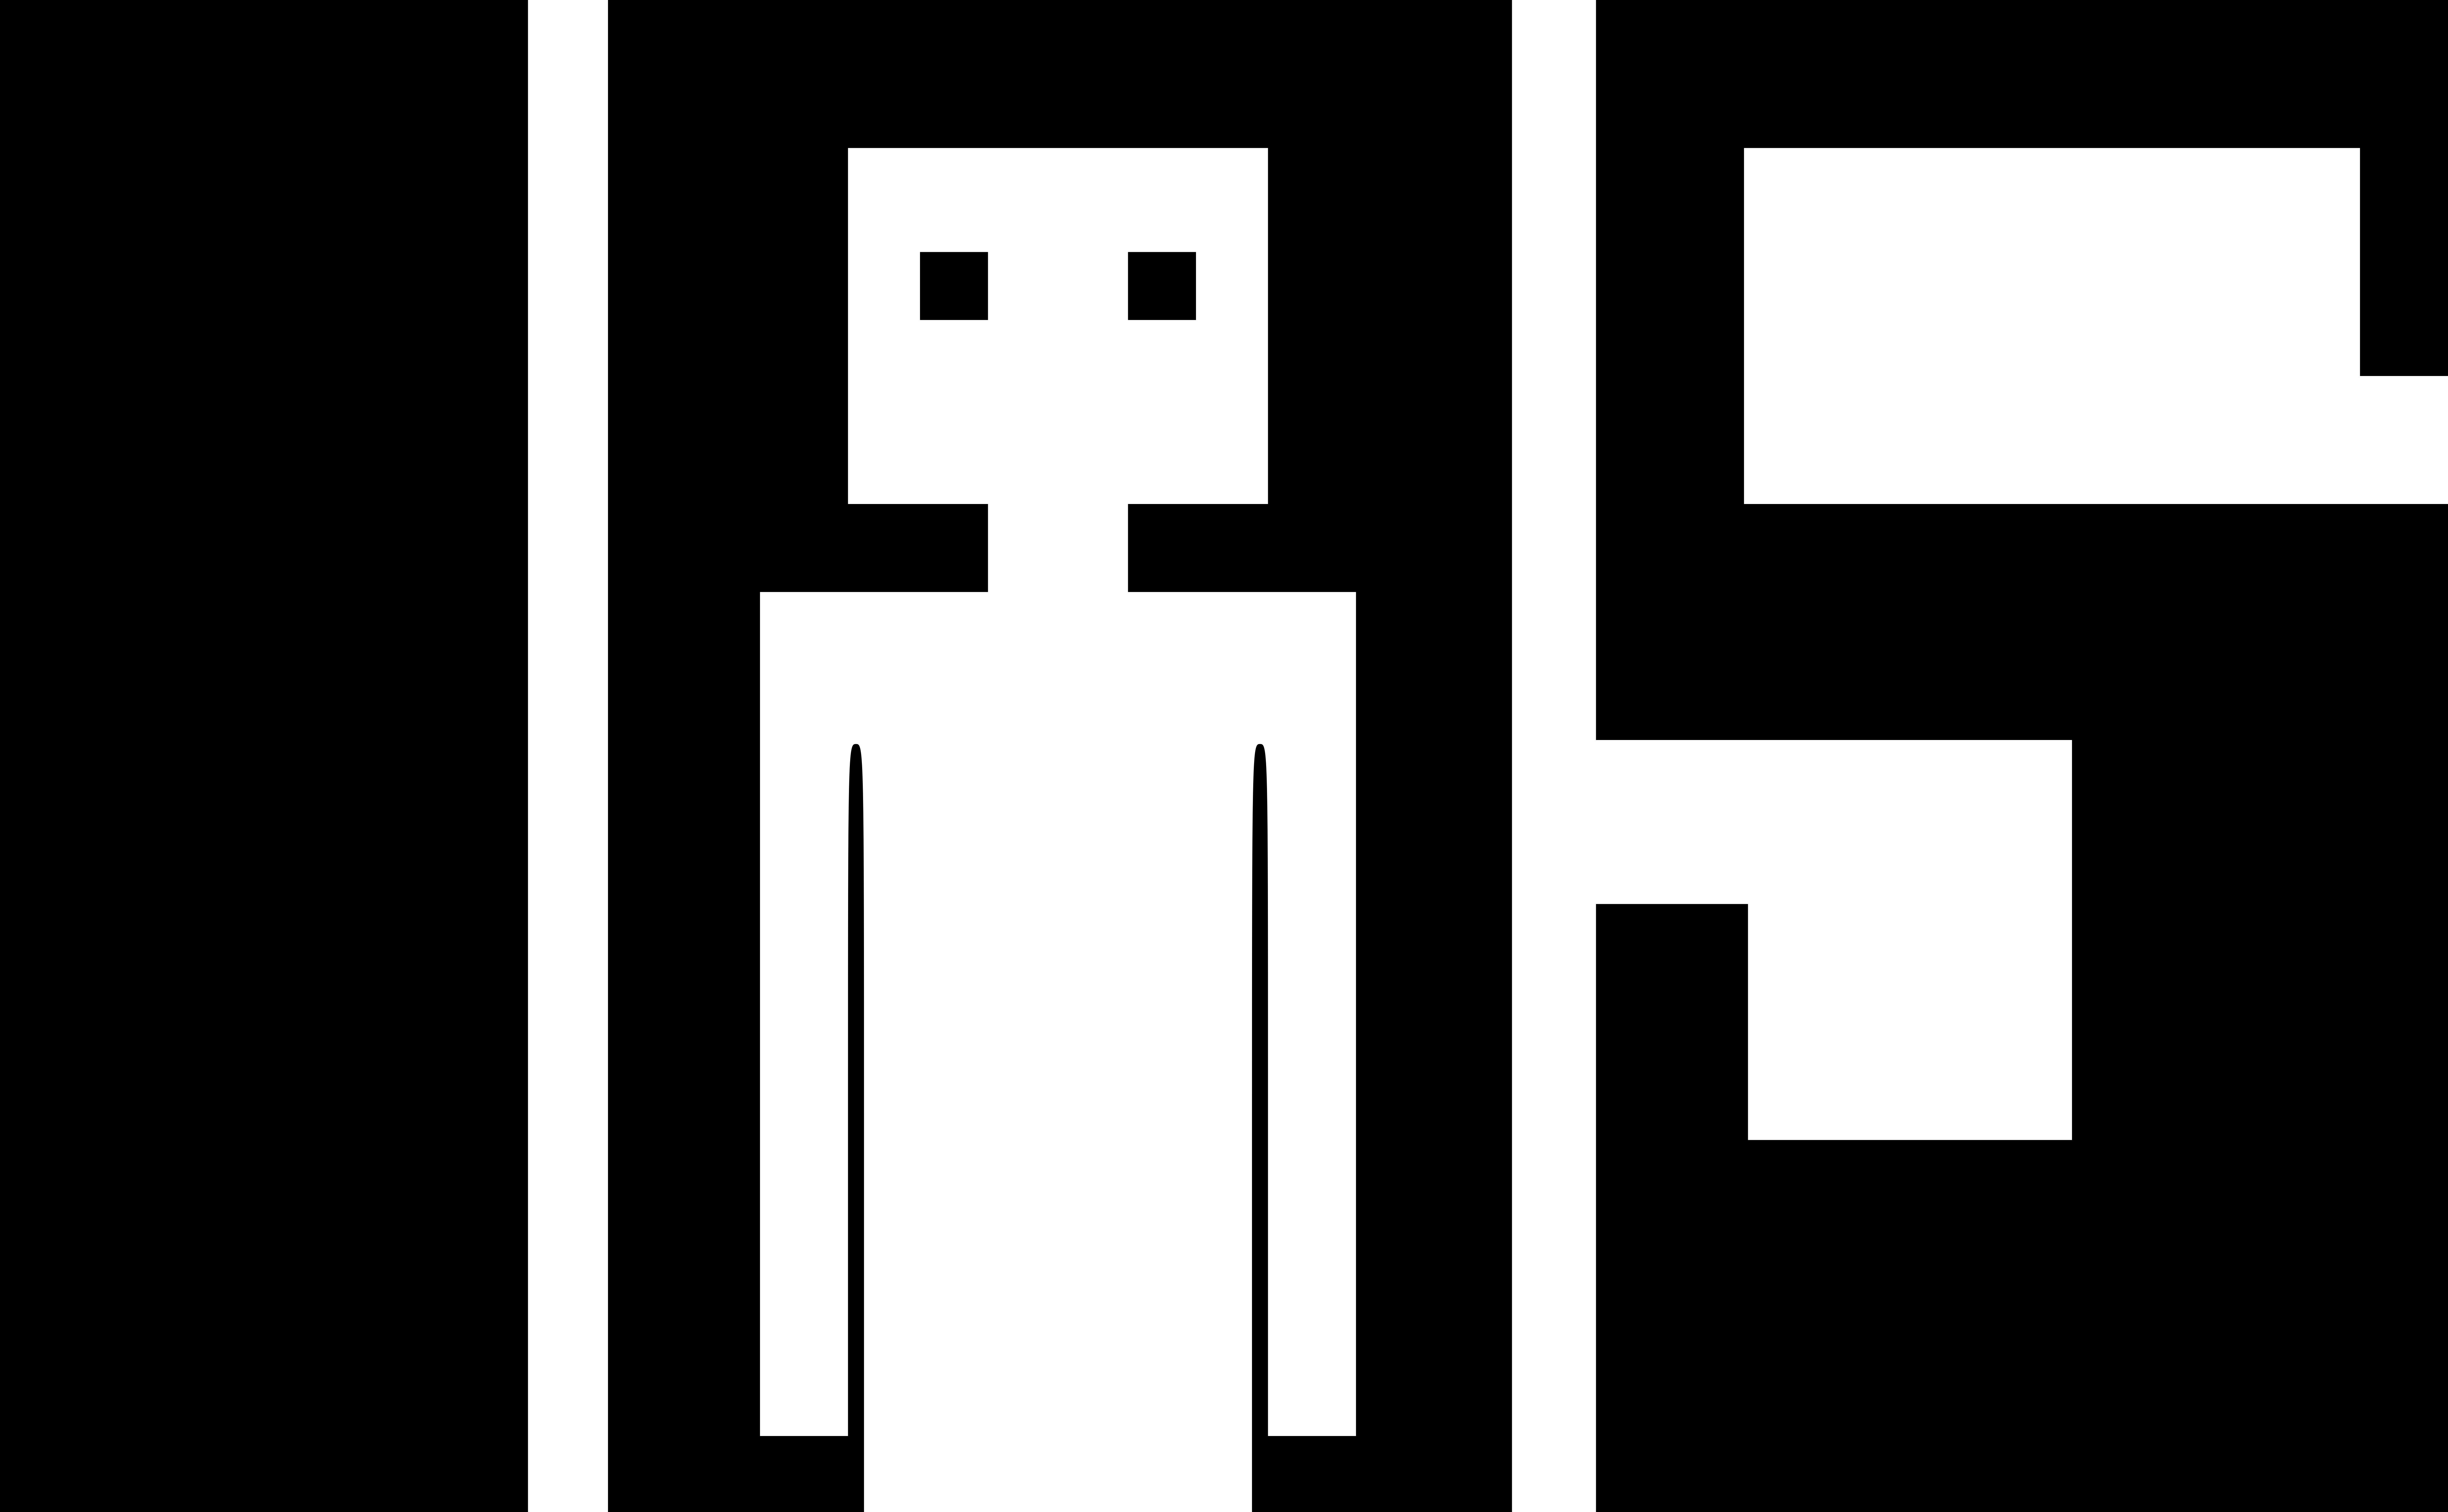
\includegraphics[width=0.5\linewidth]{logos/iasLogo.png}}
\submissiondate{\today}
\examdate{\today}

% Hinweis zur Lizenz:
% TUDa-CI verwendet momentan die Lizenz CC BY-NC-ND 2.0 DE als Voreinstellung.
% Die TU Darmstadt hat jedoch die Empfehlung von dieser auf die liberalere
% CC BY 4.0 geändert. Diese erlaubt eine Verwendung bearbeiteter Versionen und
% die kommerzielle Nutzung.
% TUDa-CI wird im nächsten größeren Release ebenfalls diese Anpassung vornehmen.
% Aus diesem Grund wird empfohlen die Lizenz manuell auszuwählen.
%\tuprints{urn=XXXXX,printid=XXXX,year=2022,license=cc-by-4.0}
% To see further information on the license option in English, remove the license= key and pay attention to the warning & help message.

% \dedication{Für alle, die \TeX{} nutzen.}

\maketitle

\affidavit
% Es gibt mit Version 3.20 die Möglichkeit ein Bild als Signatur einzubinden.
% TUDa-CI kann nicht garantieren, dass dies zulässig ist oder eine eigenhändige Unterschrift ersetzt.
% Dies ist durch Studierende vor der Verwendung abzuklären.
% Die Verwendung funktioniert so:
%\includepdf[pages=2]{unterschrift.pdf}
\tableofcontents
\listoffigures
\listoftables+

\chapter*{Abstract}
The introduction of the adjoint method for NeuralODEs\cite{neuralODE} has created new ways for physics-based trajectory predictions. In the subsequent chapters of this thesis, we look at deep learning models and methods targeted at predicting physical systems' behavior. We use the guiding light of Hamiltonian equations to dive into systems such as the harmonic oscillator and the three-body problem. We are intrigued with exploring graph neural networks' ability to be used in physics informed models: in the N-body problem and in the N-pendulum. This work tests the ability of graph neural networks to generalize the behavior from single realizations of elements at the node level of the graph. In this way, we hope to exemplify how such models can capture highly dynamic physical processes. 


\chapter{Introduction}
The intersection of physics and deep learning has never been more pronounced than it is today. With advancements in hardware and computational capabilities, we are now positioned to predict physical phenomena with unprecedented precision using deep learning techniques, particularly through physics-informed neural networks.\\
Physics-Informed Neural Networks (PINN) are neural networks  that encode model equations, like Partial Differential Equations (PDE), as a component of the neural network itself\cite{}. For example let us take Laplace equation which is defined as
\begin{eqnarray}
	\Delta u(\mathbf{x}) &= 0, &\texttt{   }\mathbf{x}\in \Omega,\mathbf{x}\in R^2\\
	u &= S &\texttt{   }\mathbf{x}\in \partial\Omega \text{     Dirichlet boundary condition},\\
	\frac{\partial u}{\partial \mathbf{n}} &= f(\mathbf{x}) &\texttt{   }\mathbf{x}\in \partial\Omega \text{     Neumann boundary condition}.
\end{eqnarray}
The Operator $\Delta$ is called as Laplace Operator and it defines $\Delta = \sum_i \frac{\partial^2}{\partial^2 x_i}.$\\
To build a PINN model we will use an Neural Network which will learn the solution $u$ and from that output we will calculate all needed derivatives, residuals and other parts for the optimization.

\begin{figure}[h!]
	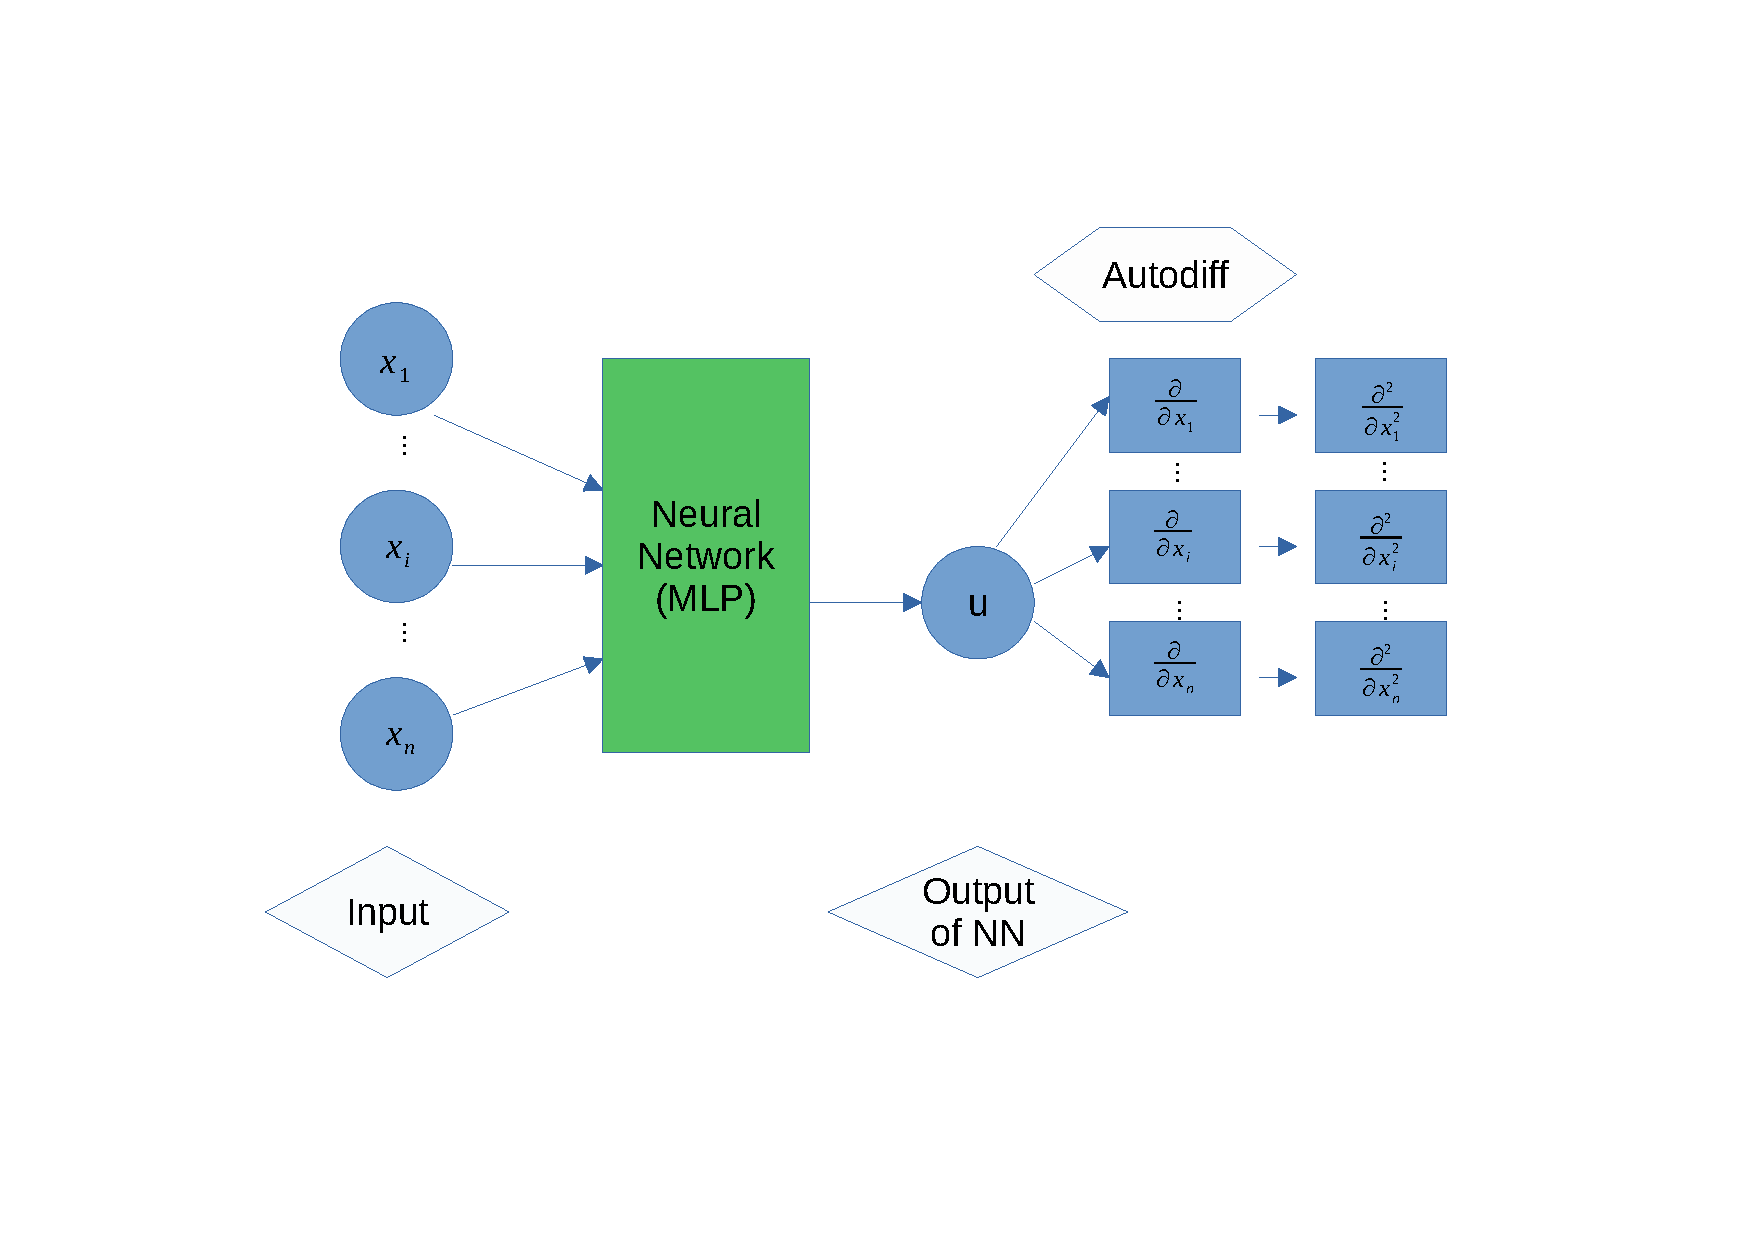
\includegraphics[width=15cm]{chapters/chapter1/pinn}
	\label{pinn}
	\caption{PINN model for Laplace Equation}
\end{figure}
In figure \ref{pinn} we can observe the architecture of such physics informed model. 
The Loss functions that we need to use to properly train our network are
\begin{eqnarray}
	\text{Loss}_s(\Theta) &=& \frac{1}{N}\sum^N_i\left(u_{\Theta}(\mathbf{x}_i)- u_i\right)^2,\\
	\text{Loss}_r(\Theta) &=& \frac{1}{R}\sum^R_i\left(\frac{\partial u_{\Theta}(\mathbf{x}_i)}{\partial x_i} - f(\mathbf{x}_i)\right)^2,\\
	\text{Loss}_l(\Theta) &=& \Delta u_{\Theta},\\
	\text{Loss}(\Theta) &=& \omega_s \text{Loss}_s +\omega_r \text{Loss}_r +\omega_l \text{Loss}_l .
\end{eqnarray}
The $\omega_s$,$\omega_r$,$\omega_l$, in this case are coefficients $0\leq \omega \leq 1$ and they are there to improve optimization capabilities which is defined as
\begin{equation}
	\Theta^* = \arg\min\text{Loss}(\Theta).
\end{equation}
The $\Theta$ are learnable parameters which can be updated with $\Theta^*$ trough optimization algorithm.\\
Such model wouldn't be possible without Automatic Differentiation\cite{} which are offered from machine learning library $\texttt{pytorch}$\cite{}. In this example we need big bunch of data and the optimization of the model could be very slow in addition if we don't have a computation capable hardware for it. Obtaining the data could be done only with exactly measurement or using some numerical solvers like FEM or Isogeometric Analysis. Don't forget, that there are Poission Equation, Wave Equation which are dependent on time $t$.\\
Those PDEs have mostly application in electrotechnical(Electro-magnetical fields) and  civil Engineering(static in construction).
In this thesis we won't work on the PDEs but similar to this topic we will try to train a model to predict the Dynamics of some physical phenomena and non-/holonomic systems of the robots.\\
The Dynamics for Robots are trivially defined as simple Second Level Ordinary Differential Equation\cite{} .
\begin{equation}
	\mathbf{M}\ddot{\mathbf{x}}(t) + \mathbf{D}(\dot{\mathbf{x}}(t)) + \mathbf{C}(\mathbf{x}(t))=0,
\end{equation} but there are other forms, as Langrange Equations of Motion if our system is holonomic\cite{}. It is based on Lagrange Function which is based on Kinetik $T$ and Potential $U$ Energy
\begin{eqnarray}
	\mathcal{L} &=& T - V,\\
	\frac{d}{dt}\frac{\partial \mathcal{L}}{\partial \dot{q}_i} - \frac{\partial \mathcal{L}}{\partial q_i}&=&0.
\end{eqnarray}   
The Lagrange Equations are used in Delan\cite{} Physics informed network and in simillar manner, but for us are most interesting to use Hamiltonian Equations of Motion.
They work for holonomic and non-holonomic systems and they are capable to build First Level Ordinary Equation
\begin{equation}
	\dot{x} = f(x,t)
\end{equation} \\
or in Hamiltonian Form where $\mathcal{H} = T + V$
\begin{equation}
	\dot{\mathbf{z}} = \mathbf{J}\frac{\partial\mathcal{H}}{\partial \mathbf{z}}
\end{equation} where $\mathbf{z}=[\mathbf{q},\mathbf{p}]^T$ and $\mathbf{J} = \begin{bmatrix}
0 & \mathbf{I}_n\\
-\mathbf{I}_n & 0
\end{bmatrix} $\\
\begin{figure}[h!]
	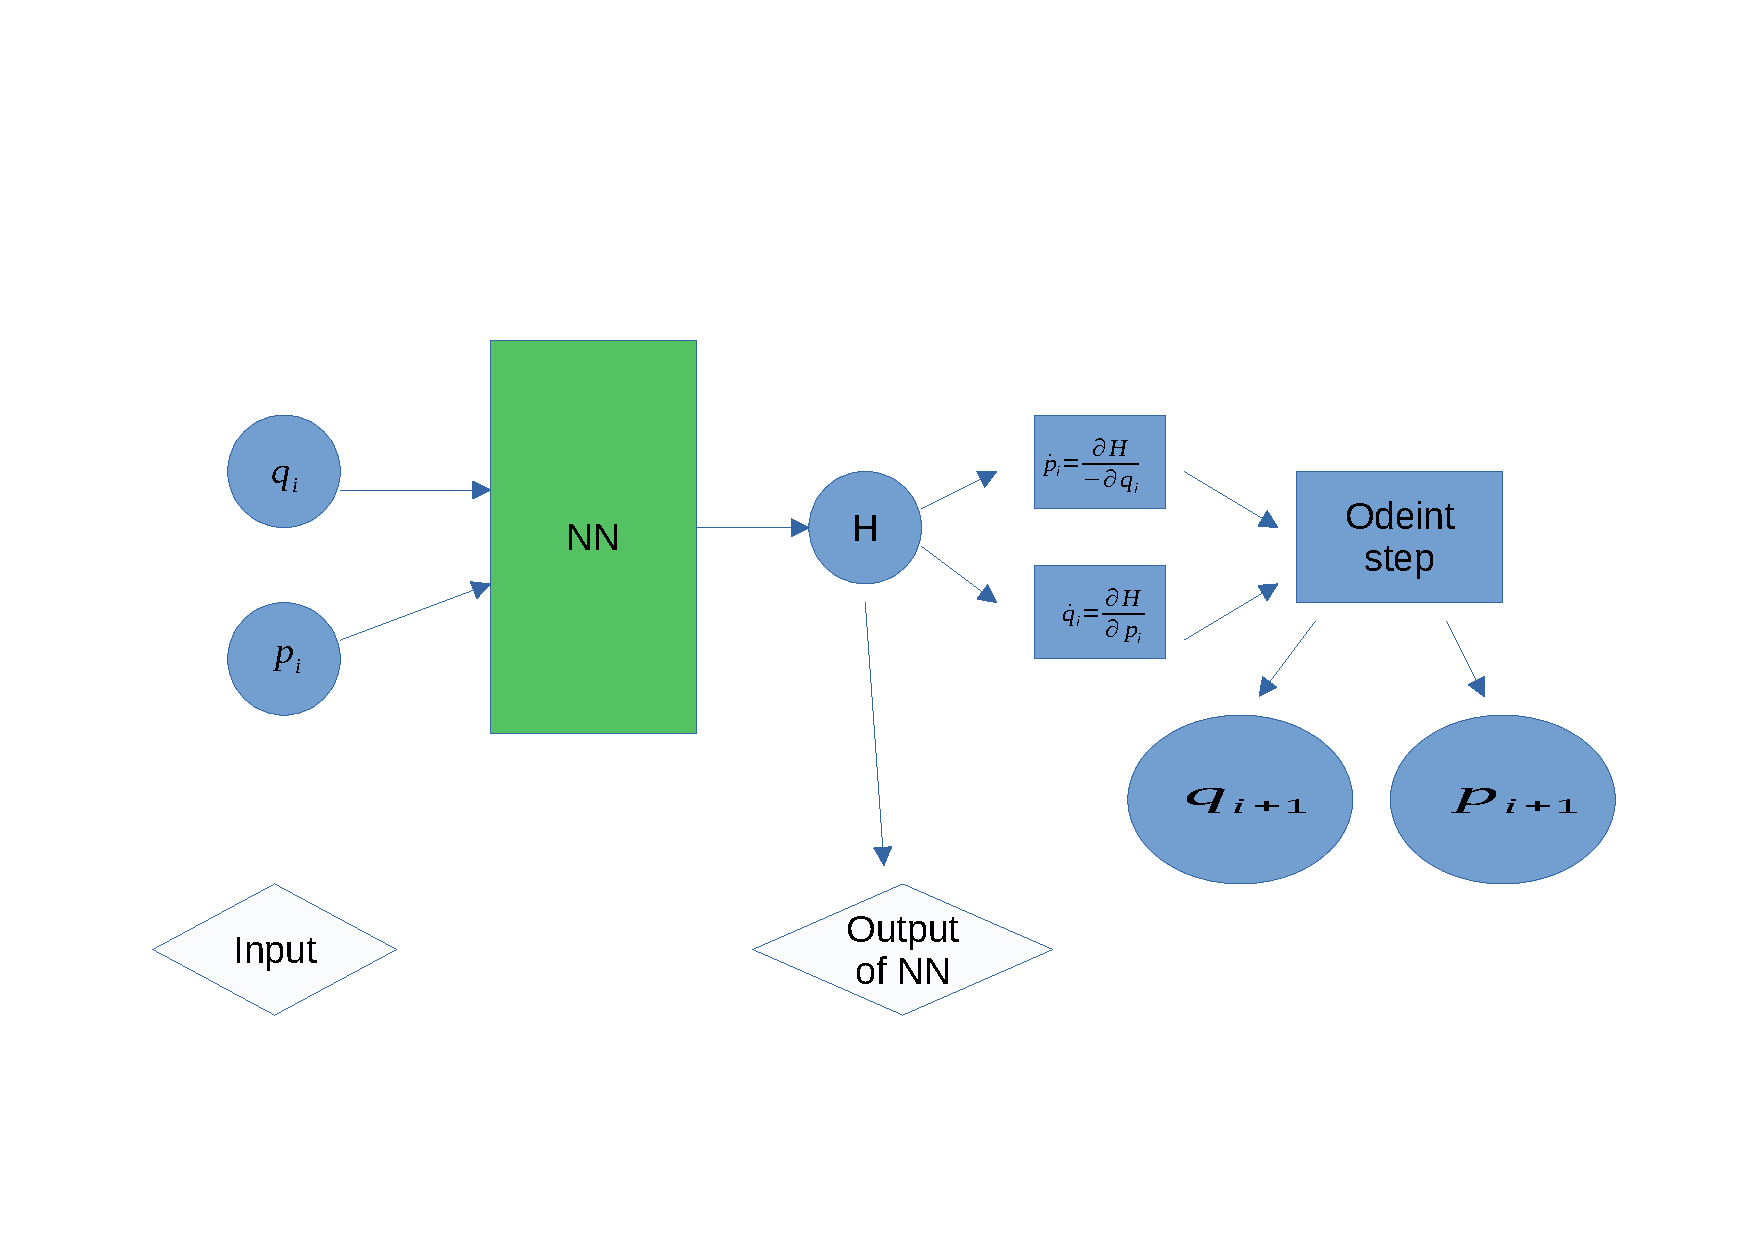
\includegraphics[width=15cm]{chapters/chapter1/hnn}
	\label{hnn}
	\caption{HNN model with integration solver step}
\end{figure}
One of such model is introduced in the \cite{} and it is called HNN. it architecture you can observe in figure \ref{hnn}.
We will make it more interesting introducing the Graph Neural Network and try to use it as a base of our architecture.\\
In this thesis we will discuss what are Hamiltonian equations and how to obtain them. In our research we stumbled upon the fact, that there are no quality datasets for training the Neural Networks which are based on physics. With this fact we brew 4 popular datasets which are based on Hamiltonian Equations of Motion.\\
Next we made new and revisit old neural architectures and test NeuralODE as new Nerual Paradigm into treaining the solutions of ODEs.\\
In the experiments we tested the capabilites of Graph Neural Networks, how do they adapt to diverse training data and their possibility to reduce or increase a degree of freedom in the training. For example how similar is the movement between 3 and 4 bodied pendulum on the same trained set of neural parameters. We hope that we will give the insight in those topics.    








%% related works, philosophy, motivations, my contributions

\chapter{Background}\label{background}
%In this chapter we will discuss main topics from Classical Mechanics and refresh out knowledge about common neural network architectures. This will be needed to understand the working of our Physics informed networks in chapter Methods.
In this chapter, we revisit some of the important concepts from Classical Mechanics and further develop an understanding of common neural network architectures. This is a critical foundation which will be required to understand how Physics-Informed Neural Networks work, as discussed in greater detail in the Methods chapter. 
\section{Classical Mechanics}\label{cs}
%The classical physics are most important science to understand the laws which govern how mass object behaves in our reality. Such science is called the Classical Mechanics. It tend to describe how the mass moves in space. Simply the movement manifests through forces applied on the matter. Sir Isaac Newton for this observed phenomena gave a laws which masses should obey  \cite{ClassPhy}
Classical Physics presents the basics for understanding the laws presiding over the behavior of objects with mass in our physical reality. This aspect of the science of Classical Mechanics describes how mass moves in space: motion is the result of forces applied to matter. Moving on, Sir Isaac Newton did develop laws that describe and predict the behavior of such objects, which today are called the Newton's Laws of Motion.\cite{ClassPhy}
\begin{itemize}
	\item Newton's 1st law: Unless acted on by an outside force the natural motion of an object is constant velocity
	\item Newton’s 2nd law: The effect of an applied force $\mathbf{F}$ upon an object of mass
	m is to induce an acceleration $\mathbf{a}$ such that $$\mathbf{F}=m\mathbf{a}$$
	If mass is constant we can introduce momentum $\mathbf{p}$.
	$$\mathbf{F}=\frac{d\mathbf{p}}{dt}$$ \\
	Derivation of the momentum in time t is a force. 
	With this equation we can obtain momentum as $$\mathbf{p}=m\mathbf{v}$$ where $\mathbf{v}$ is velocity.
	\item Newton’s 3rd law: If an object applies a force $\mathbf{F}$ on a second object, then the second object applies an equal and opposite force $-\mathbf{F}$ on the first object.\\
	In the physics it is most famous law and it is often referenced as  \textit{actio = reactio} from latin.
\end{itemize}
One of the simplest systems that adheres to these laws is the harmonic oscillator.
\subsection{Harmonic Oscilator}
Harmonic Oscilator is  system  in classical physics which describes the situation where body is displaced from equilibirium position and it experience the restoring force $\mathbf{F}$ proportional to its displacement. This system is described with Ordinary Differential Equation of second order : 
\begin{equation}
	m\ddot{\mathbf{x}}(t) = -k\mathbf{x}(t) \texttt{,   } \mathbf{x}(0)= \mathbf{x}_0
\end{equation}
We will consider this system as one dimensional $\mathbf{x}= x$
in which the harmonic motion is along straight line, the motion is said to be simple harmonic motion \cite{osci}. To show the simple harmonic motion let us solve the equation.\\
First we will build the the linear system of equations to get the first order ordinary differential equation in form: \begin{equation}
	\ddot{\mathbf{z}}= \mathbf{A}\mathbf{z} + \mathbf{b}.
\end{equation}
We are beginning with parameter $z$:
\begin{eqnarray}
	z_1 &=& x\\
	z_2 &=& \dot{x}\\
	\dot{z}_1 &=& \dot{x} = z_2\\
	\dot{z}_2 &=& \ddot{x} = -\frac{k}{m}z_1 
\end{eqnarray}
With this we got:
\begin{equation}
	\begin{bmatrix}
		\dot{z_1}\\
		\dot{z_2}\\
	\end{bmatrix} = \begin{bmatrix}
	0 & 1\\
	-\frac{k}{m} & 0\\
	\end{bmatrix}
	\begin{bmatrix}
		z_1\\
		z_2\\
	\end{bmatrix}
\end{equation}
We got differential ordinary equation which is homogeneous ($\mathbf{b}=0$). To solve this Problem we need to refresh the knowledge of solving the ODEs 

\subsection{Analytical solution of Ordinary Differential Equations}
A Differential Ordinary Equation of the first order is defined as:
\begin{equation}
\label{eq:diff}
\dot{\mathbf{z}}= \mathbf{A}\mathbf{z} + \mathbf{b}u \texttt{, }\mathbf{z}(0) = \mathbf{z}_0
\end{equation}
Before we show analytical solution of mentioned linear system, let us solve first the simplest case:
 
\begin{equation}
	\dot{z}(t)= az(t) + bu \texttt{, }z(0) = z_0
\end{equation}
Every solution of ODE has homogeneous $z_{hom}$ and particular solution $z_{par}$
\begin{equation}
	z(t) = z_{hom} + z_{par}.
\end{equation}
When we calculate de homogeneous solution we set $b=0$ and we precede with simple integration.
\begin{equation}
	\int\frac{dz}{z} = \int adt
\end{equation}
\begin{equation}
	\boxed{z_{hom}= c\exp(at)}
\end{equation}
To find particular solution we will create it with variation of the constants method.\\
We define:
\begin{equation}
	z_{part}= c(t)\exp(at)
\end{equation}
and we will put it in the differential equation
\begin{eqnarray}
	\dot{z}_{part}(t)&=& az_{part}(t) + bu(t),\\
	a\exp(at)c(t)+ \exp(at)\dot{c}(t)&=& a\exp(at)c(t) + bu(t),\\
	\dot{c}(t) &=& \exp(-at)bu(t).
\end{eqnarray}
After integration of $\dot{c}$ we get:
\begin{equation}
	\boxed{z_{part}= c(0)\exp(at) + \int^t_0 \exp(at-\tau)bu(\tau)d\tau}
\end{equation}
With inclusion of the Initial condition $z(0) = z_0$ we get final form of the solution \\
\begin{equation}
	\boxed{z= \underbrace{z_0\exp(at)}_\text{homogeneous} + \underbrace{\int^t_0 \exp(a(t-\tau))bu(\tau)d\tau}_\text{particular} }.
\end{equation}
Let so go back and solve the equation \ref{eq:diff}.\\
Obtaining the solution goes similar to simple case but it is vectorized.\\
The solution is made by homogeneous and particular solution as above.\\
\begin{equation}´
	\mathbf{z}=\mathbf{z}_{hom} + \mathbf{z}_{in}
\end{equation} 
Lets assume from the example what we have done previously that our homogeneous solution is defined as:
\begin{equation}
	\mathbf{z}_{hom}=\exp(\mathbf{A}t)\mathbf{c}
\end{equation}
This is easy to prove trough Taylor series of the $\exp(\mathbf{A}t)$.
\begin{equation}
	\exp(\mathbf{A}t) = \sum^{\infty}_{i=0}\frac{(\mathbf{A}t)î}{i!} = \mathbf{I}+ \mathbf{A}t+\mathbf{A}^2 \frac{t^2}{2!}+ \mathbf{A}^3 \frac{t^3}{3!} + \mathcal{O}(t^4)
\end{equation}
\begin{eqnarray}
	\frac{d\exp(\mathbf{A}t)}{dt} &=& \mathbf{A}+\mathbf{A}^2 t+ \mathbf{A}^3 \frac{t^2}{3!} + \mathcal{O}(t^3)=\\
	&&\mathbf{A}\left(\mathbf{I}+ \mathbf{A}t+\mathbf{A}^2 \frac{t^2}{2!}\right) + \mathcal{O}(t^3)\\
	&&\mathbf{A}\exp(\mathbf{A}t)
\end{eqnarray}
Lets put it in the equation
\begin{eqnarray}
	\dot{\mathbf{z}}_{hom}&=& \frac{d\exp(\mathbf{A}t)}{dt}\mathbf{c} =\\
	&&\mathbf{A}\exp(\mathbf{A}t)\mathbf{c} =\\
	&& \mathbf{A}\mathbf{z}_{hom}
\end{eqnarray}
and the homogeneous solution
\begin{equation}
	\boxed{
	\mathbf{z}_{hom} = \exp(\mathbf{A}t)\mathbf{c}}
\end{equation}
fulfills the equation.\\
With the variation of the constant method we obtain the particular solution:
\begin{equation}
\exp(\mathbf{A}t)\mathbf{c}(0)+ \int^t_0 \exp(\mathbf{A}(t-\tau))\mathbf{b}u(\tau)d\tau
\end{equation}
With inclusion of the initial condition $z(0) = z_0$ we get final form of the solution \\
\begin{equation}
	\boxed{\mathbf{z}= \underbrace{\exp(\mathbf{A}t)\mathbf{x}_0}_\text{homogeneous} + \underbrace{\int^t_0 \exp(\mathbf{A}(t-\tau))bu(\tau)d\tau}_\text{particular}}.
\end{equation}\\
In our work the most important part is homogeneous solution and to obtain that we should use standard practice to solving it.\\
\begin{itemize}
	\item Find eigenvalues and eigenvectors- Every matrix with full rank is diagonalizable 
	\begin{eqnarray}
		\mathbf{A} &=& \mathbf{V}\mathbf{D}\mathbf{V}^{-1}\\
		\mathbf{D} &=& \texttt{diag}(\{\lambda_1,...,\lambda_i,...\lambda_n\}) \text{    Eigenvalues}\\`
		\mathbf{V} &=& \left[\mathbf{v}_1|...|\mathbf{v}_i|...|\mathbf{v}_n\right] \text{    Eigenvectors}
	\end{eqnarray}
	It is easily obtained through characteristic polynomial $p(\lambda) =\det(\mathbf{A}-\mathbf{I}\lambda)=0$
	
	\item To find general solution we need to transform the $\dot{\mathbf{z}}= \mathbf{A}\mathbf{z}$
	\begin{eqnarray}
		\dot{\mathbf{z}} &=& \mathbf{V}\mathbf{D}\mathbf{V}^{-1}\mathbf{z}\\
		\underbrace{\mathbf{V}^{-1}\dot{\mathbf{z}}}_\text{} &=& \mathbf{D}\underbrace{\mathbf{V}^{-1}{\mathbf{z}}}_\text{}\\
		\dot{\boldsymbol{\Theta}}&=&\mathbf{D}\boldsymbol{\Theta}
	\end{eqnarray}
	This system is now trivial to solve.
	\item Set it in general solution $\Theta_i=c_i\exp(\lambda_i t)$ 
	In case of repeated eigenvalue we should use $\Theta_i=c_i \frac{t^r}{r!} \exp(\lambda_i t)$ where $r$ is number of repetitions.
	It will came up from the eigenvectors. 
	\item back-substitute $\mathbf{z}$
	\begin{eqnarray}
		\mathbf{z} &=& \mathbf{V}\boldsymbol{\Theta} =\sum^n_{i=1}\mathbf{v}_i\Theta_i\\
		\mathbf{z} &=& \sum^n_{i=1} \mathbf{v}_i\underbrace{c_i\exp(\lambda_i t)}_\text{\Theta}
	\end{eqnarray}
	\item apply initial conditions
	\begin{eqnarray}
	\mathbf{z}(0) = \sum^n_{i=1} \mathbf{v}_i c_i = \mathbf{V}\mathbf{c} &=&\mathbf{z}_0\\
	\mathbf{c} &=&\mathbf{V}^{-1}\mathbf{z}_0
    \end{eqnarray}
	
\end{itemize}

In this procedure we obtained the homogeneous solution. The particular solution is in some cases trivial but in some not solvable analytically due to $\mathbf{b}u(t)$. It is possible that it is nonlinear function. 
In those cases we use numerical methods to obtain the solutions.

\subsection{Numerical solution of Ordinary Differential Equations}
For every every ODE there is solution, sometimes there is no analytical solution but we can obtain numerical one trough numerical integrators. 
Still numerical solutions are only approximations of the analytical solution. Due to their stability we differ two categories of one-step methods and that are explicit and implicit methods.\\
\begin{itemize}
	\item explicit methods are trivial to calculate because the next step is dependent only on the previous step:
	\begin{equation}
		x(t_{i+1}) = x(t_i) + h\Phi(x(t_i)),t_i)
	\end{equation}
	\item implicit methods are chalenging because the next step is dependent on itself.
	\begin{equation}
		x(t_{i+1}) = x(t_i) + h\Phi(x(t_{i+1})),t_{i+1})
	\end{equation}
To obtain the step it is needed to know  function $\Phi$ and solving a next step trough some method like  for example Einstein-Raphson method. 
\end{itemize}
To assure the stability and correctness of the methods we need to set some properties.
The properties that the every one-step method should have, are Consistency and Convergence.\\

The Consistency are proven over local discretisation error.
Let say that for $(x,y)\in  \mu = \mu(\eta)$ is a solution for the ODE $\mu^{'} = f(\eta,\mu), \mu(x)=y$,then the discretisation error is
\begin{equation}
	le(x,y;h) = \mu(x+h)-\mu{x}-h\Phi(x,y;h)
\end{equation}
and discretisation error per step
\begin{equation}
	\Delta(x,y;h)=\frac{le(x,y;h)}{h}. 
\end{equation}
A one-step method is consistent if
\begin{equation}
	\lim_{h\rightarrow 0} \Delta(x,y;h) = 0.
\end{equation}
For the method to be convergent need to be consistent. The general definition of convergency is
\begin{equation}
\lim_{h\rightarrow 0} \Phi(x,y;h) = f(x,y)
\end{equation}
To prove this we should look for the consistency and convergency rank.
\begin{itemize}
	\item Consistency rank $p$\begin{equation}
		||\Delta(x,y;h)||\leq Kh^p
	\end{equation}
\item Convergency rank $p$
\begin{eqnarray}
	E(h) &=& \max_{j=0,1,...N}||y_j-y(x_j)||\text{ global discretisation error }\\
	\lim_{h\rightarrow 0}E(h) &=& 0 \text{ Convergence}\\
	E(h) &\leq&  Kh^p
\end{eqnarray}



\end{itemize} 
This properties are highly important to know because we will use for the experiments mostly the Runga-Kutta methods which are based on those properties.\\
Most important for us are
\begin{itemize}
	\item Euler method
		\begin{equation}
			x_{i+1} = x_i + hf(x_i,t_i)
		\end{equation}
	\item Runge-Kutta 4 Method(RK4)
		\begin{eqnarray}
			K_1 &=& f(x_i,t_i)\\
			K_2 &=& f(x_i + \frac{h}{2}K_1,t_i +\frac{h}{2})\\
			K_3 &=& f(x_i + \frac{h}{2}K_2,t_i+\frac{h}{2})\\
			K_4 &=& f(x_i + hK_3,t_i +h)\\
			x_{i+1} &=& x_i + \frac{h}{6}(K_1 + 2K_2 +2K_3 +K_4)
		\end{eqnarray}	
	\item Dormand- Prince method is most accurate method for obtaining he solutions of ODEs\cite{dopri5}.
	It is widely used in experiments.\\
		
\end{itemize}
\subsection{Solving the harmonic oscilator}
In one of the previous subsections we obtained the first order ODE for harmonic oscilator and we described how it should be solved.
\begin{equation}
	\begin{bmatrix}
		\dot{z_1}\\
		\dot{z_2}\\
	\end{bmatrix} = \begin{bmatrix}
		0 & 1\\
		-\frac{k}{m} & 0\\
	\end{bmatrix}
	\begin{bmatrix}
		z_1\\
		z_2\\
	\end{bmatrix}\text{   , }\mathbf{z}_0 = \begin{bmatrix}
x_0\\
v_0\\
\end{bmatrix}
\end{equation}
Through the system Matrix $A = \begin{bmatrix}
	0 & 1\\
	-\frac{k}{m} & 0\\
\end{bmatrix}$ we got complex eigenvalues, which are $\lambda_1 = i\sqrt{\frac{k}{m}}$ and $\lambda_2 = -i\sqrt{\frac{k}{m}}$.\\
General solution of this problem is
\begin{equation}
	z_1 = x = c_1\exp(i\sqrt{\frac{k}{m}}t) + c_2\exp(i\sqrt{-\frac{k}{m}}t)
\end{equation}
With applying of the euler formula:
\begin{equation}
	\exp(iat)=\cos(at) + i\sin(at)
\end{equation}
We get simplified solution
\begin{eqnarray}
	z_1 &= x =& (c_1+c_2)\cos\left(\sqrt{\frac{k}{m}}t\right) + (c_1-c_2)i\sin\left(\sqrt{\frac{k}{m}}t\right)\\
	z_2 &= \dot{x} =& -(c_1+c_2)\sqrt{\frac{k}{m}}\sin\left(\sqrt{\frac{k}{m}}t\right)+(c_1-c_2)\sqrt{\frac{k}{m}}i\cos\left(\sqrt{\frac{k}{m}}t\right).
\end{eqnarray}
Now we can apply initial conditions
\begin{eqnarray}
x(0)=x_0 = c_1 + c_2,\\
\dot{x}(0)=v_0 = i(c_1-c_2).
\end{eqnarray}
The velocity in our cases is an real number which we can assume that constants $c_1$ and $c_2$ are equal. 
This simplifies our equations  and we can substitute $x_0 = c_1 +c_2$
\begin{eqnarray}
	z_1 &= x =& x_0\cos\left(\sqrt{\frac{k}{m}}t\right),\\
	z_2 &= \dot{x} =& -x_0\sqrt{\frac{k}{m}}\sin\left(\sqrt{\frac{k}{m}}t\right)
\end{eqnarray}
The is harmonic at we can se that clearly because it is periodic and we can read an angle velocity of periodic movement $\omega = \sqrt{\frac{k}{m}}$,
\begin{eqnarray}
	z_1 &= x =& x_0\cos\left(\omega t\right)\\
	z_2 &= \dot{x} =& -x_0\omega\sin\left(\omega t\right)
\end{eqnarray}
\subsection{Langrange and Hamiltonian Equations}
In robotics, research and model creation of the robot models are not only one-bodied system. Mostly they are are rigid-body systems like a manipulator which has N degrees of freedom. Every of the joints and links have own properties like mass, friction, etc.\\
The Kinematic of the model and irreversibility is possible to calculate with mathematic methods. Kinematic is just establishing the function which with correct input like angles of joints $q$ give as an output in form of target position of the endeffector. This easy easy to establish with Denavit–Hartenberg convention.  On the other hand determining Dynamics is not trivial task. The Dynamic creates trajectory which is in form of ODE.\\
There is one most popular method to solve and establish Dynamics of the model and that are Lagrange Equations.
\subsubsection{Lagrange Equations}
Langrage Equations are derived from D’Alambert Principle which is an alternative to the Newton's second law\cite{ClassPhy}:
\begin{equation}
	\mathbf{F} = m\mathbf{a}
\end{equation}   
In the case of the rigid body:
\begin{equation}
	\mathbf{F}_i = \sum_i{m_i \mathbf{a}_i}
\end{equation}
To derive Lagrangian Equations which describes dynamics we need first to define constraints. Let us define homonomic constraints.
For $N$ bodies B = $\{\mathbf{r}_1,...,\mathbf{r}_i,...,\mathbf{r}_N\}\text{ ; } \mathbf{r}_i=\mathbf{r}_i(q_1,...,q_i,...,q_n, t)$
\begin{equation}
	\boxed{G_k(\mathbf{r}_1,..,\mathbf{r}_i,..,\mathbf{r}_n,t)=0\text{ for}k=1,..M}
\end{equation}
Where the $q_i$ are generalized coordinates and the
parameters are also constrained as $3\cdot M\cdot N = n$.\\
In case of two dimensional N-Pendulum some of that constraints would look like:
\begin{equation}
	G_i := \left|\left|\mathbf{r}_i - \mathbf{r}_{i+1}\right|\right| - d_i = 0
\end{equation}
This says that the distance between two neighboring joints are constant.
holonomic constraint defines the relation between bodies $\r_i$ on some configuration space $\mathcal{A}$.
Lets go back to the second newton law and lets apply holonomic constraint. With holonomic constraint we can spilt $\mathbf{F}$ on constraint force $\mathbf{F}^c$ and apllied force $\mathbf{F}^a$.
\begin{equation}
	\mathbf{F} =\mathbf{F}^c + \mathbf{F}^a
\end{equation}
Now we will apply virutal Work principle, which comes from orthogonality of virtual displacement and constraint forces \cite{ortho}
\begin{equation}
	\boxed{\sum_i{\mathbf{F}_i^c \cdot \underbrace{\delta \mathbf{r}_i}=0}_\text{virtual displacement}}
\end{equation}
to the constrained Newton's second law we get following formula which is D'Alambert principle\cite{dalam}:
\begin{eqnarray}
	 \mathbf{F}^c_i &=& \mathbf{F}_i- \mathbf{F}^a_i\\
	 \sum_i{\mathbf{F}_i^c \cdot \delta \mathbf{r}_i} &=& \sum_i{(\mathbf{F}_i- \mathbf{F}^a_i) \cdot \delta \mathbf{r}_i}\\
	 \sum_i{(\mathbf{F}_i- m_i\ddot{\mathbf{r}}_i) \cdot \delta \mathbf{r}_i}&=&0\text{    D'Alambert Principle}
\end{eqnarray}\\
If we need virtual displacement for the generalized coordinates:
\begin{equation}
	\delta\mathbf{r}_i = \sum_j^n{\frac{\partial\mathbf{r}_i}{\partial q_j}\cdot \delta q_j}
\end{equation}
Now we can derive Langrange Equations applying last equation to D'Alambert principle:
\begin{eqnarray*}
\sum_i^N{\mathbf{F}_i \cdot \delta \mathbf{r}_i} &=& \\ \sum_i^N{\mathbf{F}_i\sum_j^n{\frac{\partial\mathbf{r}_i}{\partial q_j}\cdot \delta q_j}}&=&\\
\sum_j^n{\delta q_j\underbrace{\sum_i^N{\mathbf{F}_i}\frac{\partial\mathbf{r}_i}{\partial q_j}}_\text{$Q_j$}}&=&\boxed{\sum_j^n{\delta q_j\cdot Q_j}}\\
\sum_i^N{m_i\ddot{\mathbf{r}}_i \cdot \delta \mathbf{r}_i}&=&\\
\sum_i^N{m_i\ddot{\mathbf{r}}_i \sum_j^n{\frac{\partial\mathbf{r}_i}{\partial q_j}\cdot \delta q_j}}&=&
\sum_j^n{\delta q_j\sum_i^N{m_i\ddot{\mathbf{r}}_i\frac{\partial\mathbf{r}_i}{\partial q_j}}}\\
\text{with substitution of: } \frac{\partial\dot{\mathbf{r}_i}}{\partial \dot{q_j}} &=& \frac{\partial}{\partial \dot{q_j}}\left(\frac{d\mathbf{r}_i}{dt} + \sum^N_i{\frac{\partial \mathbf{r_i}}{q_j}\dot{q_j}}\right) = \frac{\partial \mathbf{r_i}}{q_j}\\
\sum_i^N{m_i\ddot{\mathbf{r}}_i \sum_j^n{\frac{\partial\mathbf{r}_i}{\partial q_j}\cdot \delta q_j}}&=&
\sum_j^n{\delta q_j\sum_i^N{m_i\ddot{\mathbf{r}}_i\frac{\partial\dot{\mathbf{r}_i}}{\partial \dot{q_j}}}}\\
\text{with: }\sum_i^N{\frac{d}{dt}m_i\dot{\mathbf{r}}_i\frac{\partial\dot{\mathbf{r}_i}}{\partial \dot{q_j}}} &=& \sum_i^N{m_i\ddot{\mathbf{r}}_i\frac{\partial\dot{\mathbf{r}_i}}{\partial \dot{q_j}}+m_i\dot{\mathbf{r}_i}\frac{d}{dt}\frac{\partial \mathbf{r}_i}{\partial q_j}}\\
\sum_j^n{\delta q_j\sum_i^N{m_i\ddot{\mathbf{r}}_i\frac{\partial\mathbf{r}_i}{\partial \dot{q_j}}}} &=& \sum_j^n{\delta q_j\sum_i^N{\frac{d}{dt}\left(m_i\dot{\mathbf{r}_i}\frac{\partial\dot{\mathbf{r}_i}}{\partial \dot{q}}\right)-m_i\dot{\mathbf{r}_i}\frac{\partial\dot{\mathbf{r}_i}}{\partial q}}}\\
\end{eqnarray*}
We get this equation
\begin{equation}
\boxed{\sum_i^N{m_i\ddot{\mathbf{r}}_i \cdot \delta \mathbf{r}_i} =\sum_j^n{\delta q_j\left[\frac{d}{dt}\frac{\partial}{\partial \dot{q_j}}\left(\sum_i^N\frac{1}{2}m_i\dot{\mathbf{r}_i}^2\right)-\frac{\partial}{\partial \dot{q_j}}\left(\sum_i^N\frac{1}{2}m_i\dot{\mathbf{r}_i}^2\right)\right]}}
\end{equation}
With those two made equations we can finally put it togehter in D'Alambert Principle formula:
\begin{equation}
	\sum_j^n{\delta q_j\left[\frac{d}{dt}\frac{\partial}{\partial \dot{q_j}}\left(\sum_i^N\frac{1}{2}m_i\dot{\mathbf{r}_i}^2\right)-\frac{\partial}{\partial q_j}\left(\sum_i^N\frac{1}{2}m_i\dot{\mathbf{r}_i}^2\right)- Q_j\right]} =0 
\end{equation}
This Equation is almost complete, we need to define the energies and their specifications

\begin{itemize}
	\item Kinetic Energy - Energy possessed by bodies due to their motion.\\
	The Formula for kinetic energy is
	\begin{equation}
		T(q,\dot{q}) = \sum_i^N\frac{1}{2}m_i\dot{\mathbf{r}_i}^2
	\end{equation}
	\item Potential Energy - Energy held by body becuase of its relative position to other bodies or other target.\\
	There is many types of potential energy:\\
	Pendelum - $U(q=h)=mgh$\\
	Oscilator - $U(q)=\frac{kq}{2}$ 
\end{itemize}
In the Formula $\mathbf{Q}$ is generalized force and it is created from the gradient of the potential energy and it is conservative :
\begin{equation}
	\mathbf{Q_j} =- \sum^N_i \nabla_{\mathbf{r_i}}U(q)\frac{\partial\mathbf{r_i}}{\partial q_j}= -\frac{\partial U}{\partial q_j}
\end{equation} 
Potential Energy is only dependent on position of the bodies $\frac{\partial U}{\partial \dot{q}} = 0$.\\
The Lagrange Equations for holonomic constrains and conservative force is defined as:
\begin{eqnarray}
\frac{d}{dt}\frac{\partial}{\partial \dot{q_j}}\left(T-U\right)-\frac{\partial}{\partial q_j}\left(T-U\right) =0\\
\frac{d}{dt}\frac{\partial}{\partial \dot{q_j}}\mathcal{L}-\frac{\partial}{\partial q_j}\mathcal{L} =0
\end{eqnarray}
$\mathcal{L}$ is called Lagrangian.
\subsubsection{Hamiltonian Equations}
To derive Hamiltonian Equations we need an Lagrangian $\mathcal{L}$.
We have two famous derivation of Langrangian and that are:
\begin{equation}
	\frac{\partial\mathcal{L}}{\partial \mathbf{q}} = \dot{\mathbf{p}}
\end{equation}
\begin{equation}
	\frac{\partial\mathcal{L}}{\partial \dot{\mathbf{q}}} = \mathbf{p}
\end{equation}
Through Legendre Transformation we can obtain Hamiltonian $\mathcal{H}$
\begin{equation}
	\mathcal{H}(\mathbf{q},\dot{\mathbf{q}},\mathbf{p},t) = \sum_i^N  \dot{\mathbf{q}_i} \cdot \mathbf{p}_i -\mathcal{L}(\mathbf{q},\dot{\mathbf{q}},t)
\end{equation}
With total derivation\cite{ham} we get
\begin{eqnarray}
	d\mathcal{H} &=& \sum_i^N\left[ \dot{\mathbf{q}} d\mathbf{p}_i +  \mathbf{p}_i d\dot{\mathbf{q}_i} - \frac{\partial\mathcal{L}}{\partial \mathbf{q}_i} d\mathbf{q}_i - \frac{\partial\mathcal{L}}{\partial \dot{\mathbf{q}_i}} d\dot{\mathbf{q}_i}\right] - \frac{\partial\mathcal{L}}{\partial t} dt\\ 
	&=& \sum_i^N\left[ \dot{\mathbf{q}} d\mathbf{p}_i +  \mathbf{p}_i d\dot{\mathbf{q}_i} - \dot{\mathbf{p}_i} d\mathbf{q}_i - \mathbf{p}_i d\dot{\mathbf{q}_i}\right] - \frac{\partial\mathcal{L}}{\partial t} dt\\
	&=&\sum_i^N\left[ \dot{\mathbf{q}} d\mathbf{p}_i  - \dot{\mathbf{p}_i} d\mathbf{q}_i\right] - \frac{\partial\mathcal{L}}{\partial t} dt\\
\end{eqnarray}
On the other hand we want hamiltonian which is dependent on canoical moment and generalized coordinates $\mathcal{H}=\mathcal{H}(\mathbf{q},\mathbf{p},t)$
In that case the total derivation of Hamiltonian $\mathcal{H}$ is
\begin{equation}
	d\mathcal{H} = \sum_i^N\left[\frac{\partial \mathcal{H}}{\partial \mathbf{q}_i}d\mathbf{q}_i + \frac{\partial \mathcal{H}}{\partial \mathbf{p}_i}d\mathbf{p}_i\right] + \frac{\partial\mathcal{H}}{\partial t} dt
\end{equation}
With comparing both equivalent derivations we can define the equations of motion:
\begin{equation}
	\dot{\mathbf{p}} = -\frac{\partial \mathcal{H}}{\partial \mathbf{q}}
\end{equation}
\begin{equation}
	\dot{\mathbf{q}} = \frac{\partial \mathcal{H}}{\partial \mathbf{p}}
\end{equation}
\begin{equation}
	\frac{\partial\mathcal{H}}{\partial t} = - \frac{\partial\mathcal{L}}{\partial t}
\end{equation}
Hamiltonian equations are very useful because in the case $\frac{\partial\mathcal{H}}{\partial t} = 0$ our Total Energy $\mathcal{H} = E = T + U$ is conserved and often we can derive time independent motion.
\section{Neural Network Architectures}
At the beginning of our research we experimented with feedforward networks and recurrent networks.  
\subsection{Deep forward Network - Multilayer Perceptron }
Feedforward networks like Multilayer perceptron approximates a certain function $\mathbf{f(\mathbf{x})}$. As MLP function we will show it as a mapping $\mathbf{f}(\mathbf{x}|\Theta)$.\\
The main goal of feedforward network is to fit the model so that the we get best approximation. Fit the model means to learn the parameters of the model trough optimizing procedure.\\
Multiplayer perceptron is fully connected feedforward neural network. The nodes of the MLP are often called neurons and they build a layer. A minimal MLP has three consecutive layers: which form complete bipartite graph.\\
Mathematical expression of one neuron:
\begin{equation}
	y = \sigma(\sum_i{w_i \cdot x_i} + b) 
\end{equation}
Mathematical expression of the feedforward layer network:
\begin{equation}
	\mathbf{h}^{(k+1)} =\sigma\left(\mathbf{W}^{(k)}\mathbf{h}^{(k)} + \mathbf{b}^{(k)}\right)
\end{equation} and we can see graphical representation in \ref{mlp}
In this equation $\sigma$ is called activation function, 
$\mathbf{W}$ as weights and $\mathbf{b}$ as bias which are our parameters $\Theta =\{\mathbf{W},\mathbf{b}\}$.\\
\begin{figure}[h!]
	\centering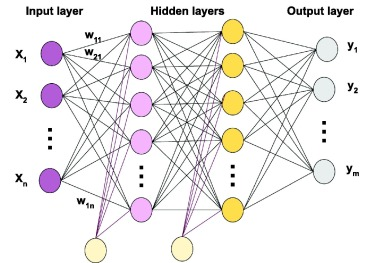
\includegraphics[width=8cm]{chapters/chapter2/mlp}
	\caption{Multilayer perceptron\cite{mlppic}}
	\label{mlp}
\end{figure}
The activation function in the network introduces non linearity to improve approximation capability.\\




\subsection{Recurrent Neural Networks}
Reccurent Neural Networks are very interesting concept of Neural Network architecture. It is mostly used for speech recognition but for a time series\cite{mlprnn}.\\
Architecture of this Neural Network depends on which data we work.
There is three types which we can use\cite{rnntypes}:
\begin{itemize}
	\item many to many\\
	This type is used for speech recognition we use a dataset which has sentences and it outputs some values which could be understood from other model. Fo example translation or video captioning
	\item one to many\\
	used for the time series data from one input we can create recurrence that represent a time point with new output. From one input we get more outputs. time-series can be for example music generation.
	\item many to one\\
	from many outputs we get only one output. This is very good model for example spam detection
\end{itemize}
Let say that we have a sequence $S = \{\mathbf{x}^0,\mathbf{x}^1,...,\mathbf{x}î,..\mathbf{x}^n\}$. the first element $\mathbf{h}^0$ will be initialized as 0.
The architecture of the RNN-cell\cite{rnn} described in mathematical formulation 
\begin{eqnarray*}
	\mathbf{h}^{(i)} &=& \sigma(\mathbf{W}_{hh} \cdot \mathbf{h}^{(i-1)} + \mathbf{W}_{hx}\mathbf{x}^{(i-1)} + \mathbf{b}_h)\\
	\mathbf{y}^{(i)} &=& \sigma(W_{yh}\cdot \mathbf{h}^{(i)} + \mathbf{b}_y)
\end{eqnarray*} and graphical appearance is shown in \ref{rnn}
\begin{figure}[h!]
	\centering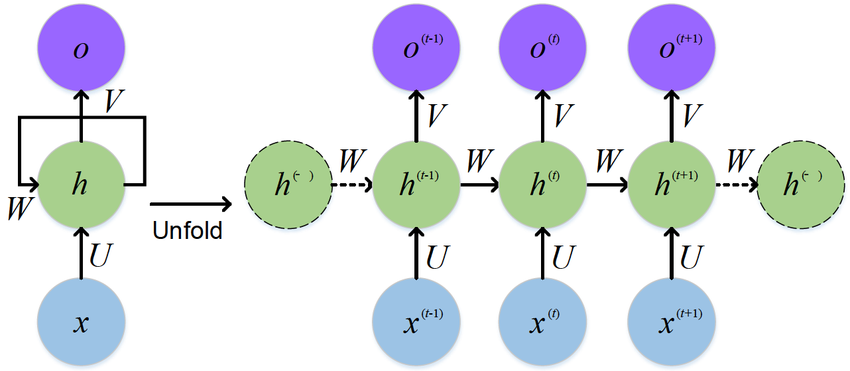
\includegraphics[width=8cm]{chapters/chapter2/rnn}
	\caption{Recurrent neural unit(many to many)\cite{rnn_picture}}
	\label{rnn}
\end{figure}

There is similar and better model then RNN and that is Gated Recurrent Unit called GRU.
We use it in same way as RNN but it his own unique architecture\cite{gru}:
\begin{eqnarray}
	r_t &=& \sigma(W_{ir} x_t + b_{ir} + W_{hr} h_{(t-1)} + b_{hr}) \\
	z_t &=& \sigma(W_{iz} x_t + b_{iz} + W_{hz} h_{(t-1)} + b_{hz}) \\
	n_t &=& \tanh(W_{in} x_t + b_{in} + r_t \odot (W_{hn} h_{(t-1)}+ b_{hn})) \\
	h_t &=& (1 - z_t) \odot n_t + z_t \odot h_{(t-1)}
\end{eqnarray} and we can see it in plot \ref{gru}
\begin{figure}[h!]
	\centering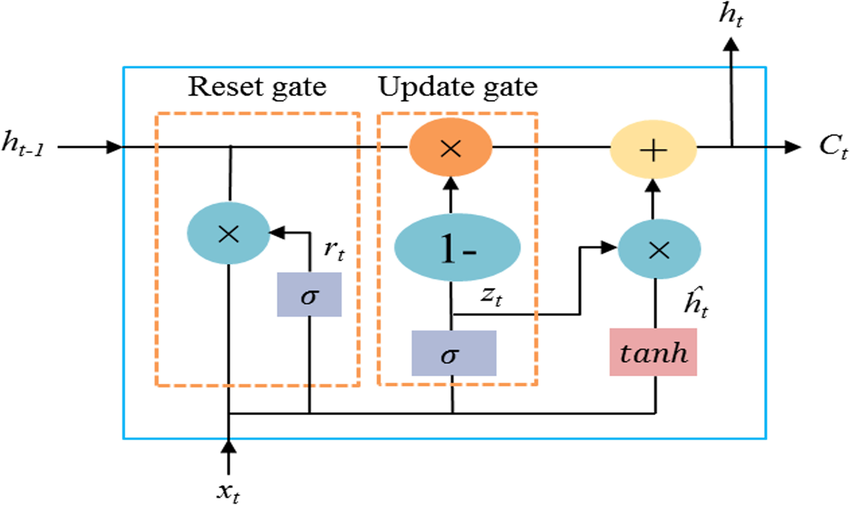
\includegraphics[width=8cm]{chapters/chapter2/gru}
	\caption{Gated recurrent unit\cite{gru_picture}}
	\label{gnn}
\end{figure}
The GRU unit is specific because it has reset gate $r_i$ and update gate $u_i$. Such architecture give better performance then at simple RNN.

\subsection{Activation functions and Loss functions}
In every neural architecture there is a activation function.
Most used activation functions are:
\begin{itemize}
	\item ReLU\\
	\begin{equation}
		\text{ReLU}(x) = max(x,0)
	\end{equation}
	This function passes only positive values.\\
	\begin{figure}[h!]
		\centering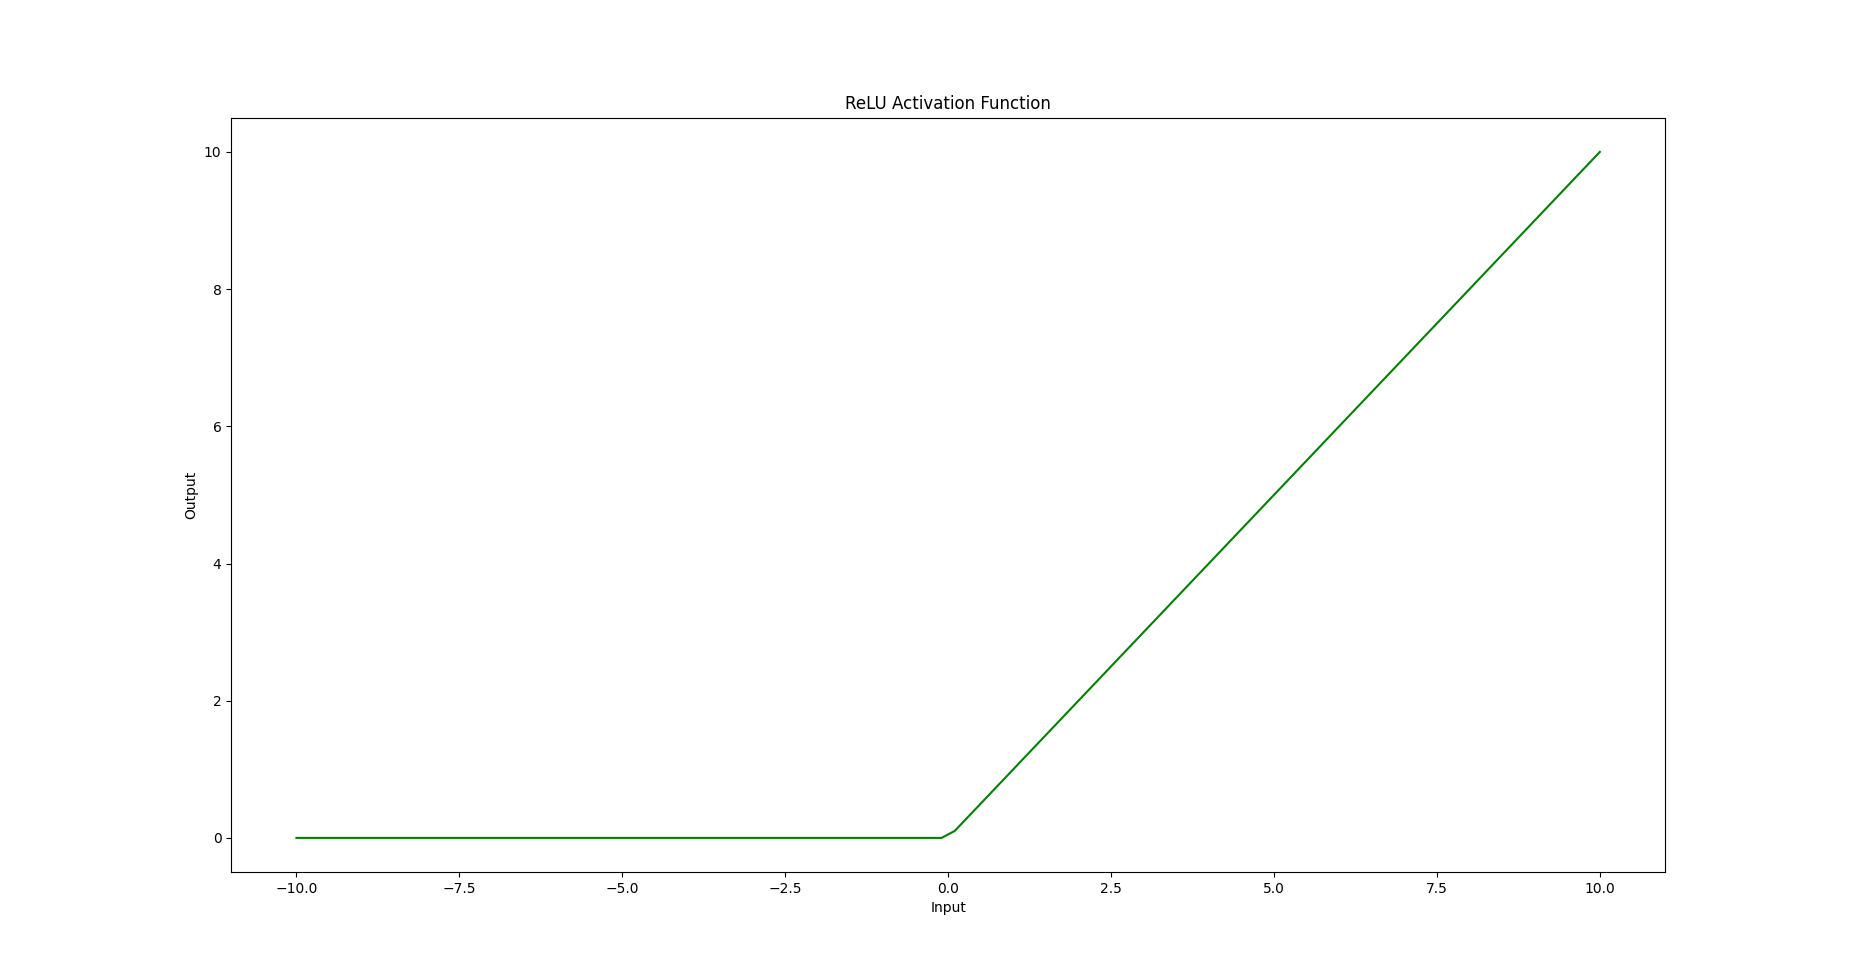
\includegraphics[width=8cm]{chapters/chapter2/relu}
		\caption{ReLU activation}
		\label{relu}
	\end{figure}
	\item tanH - It gives an output $y \in [-1,1]$\\
	\begin{figure}[h!]
		\centering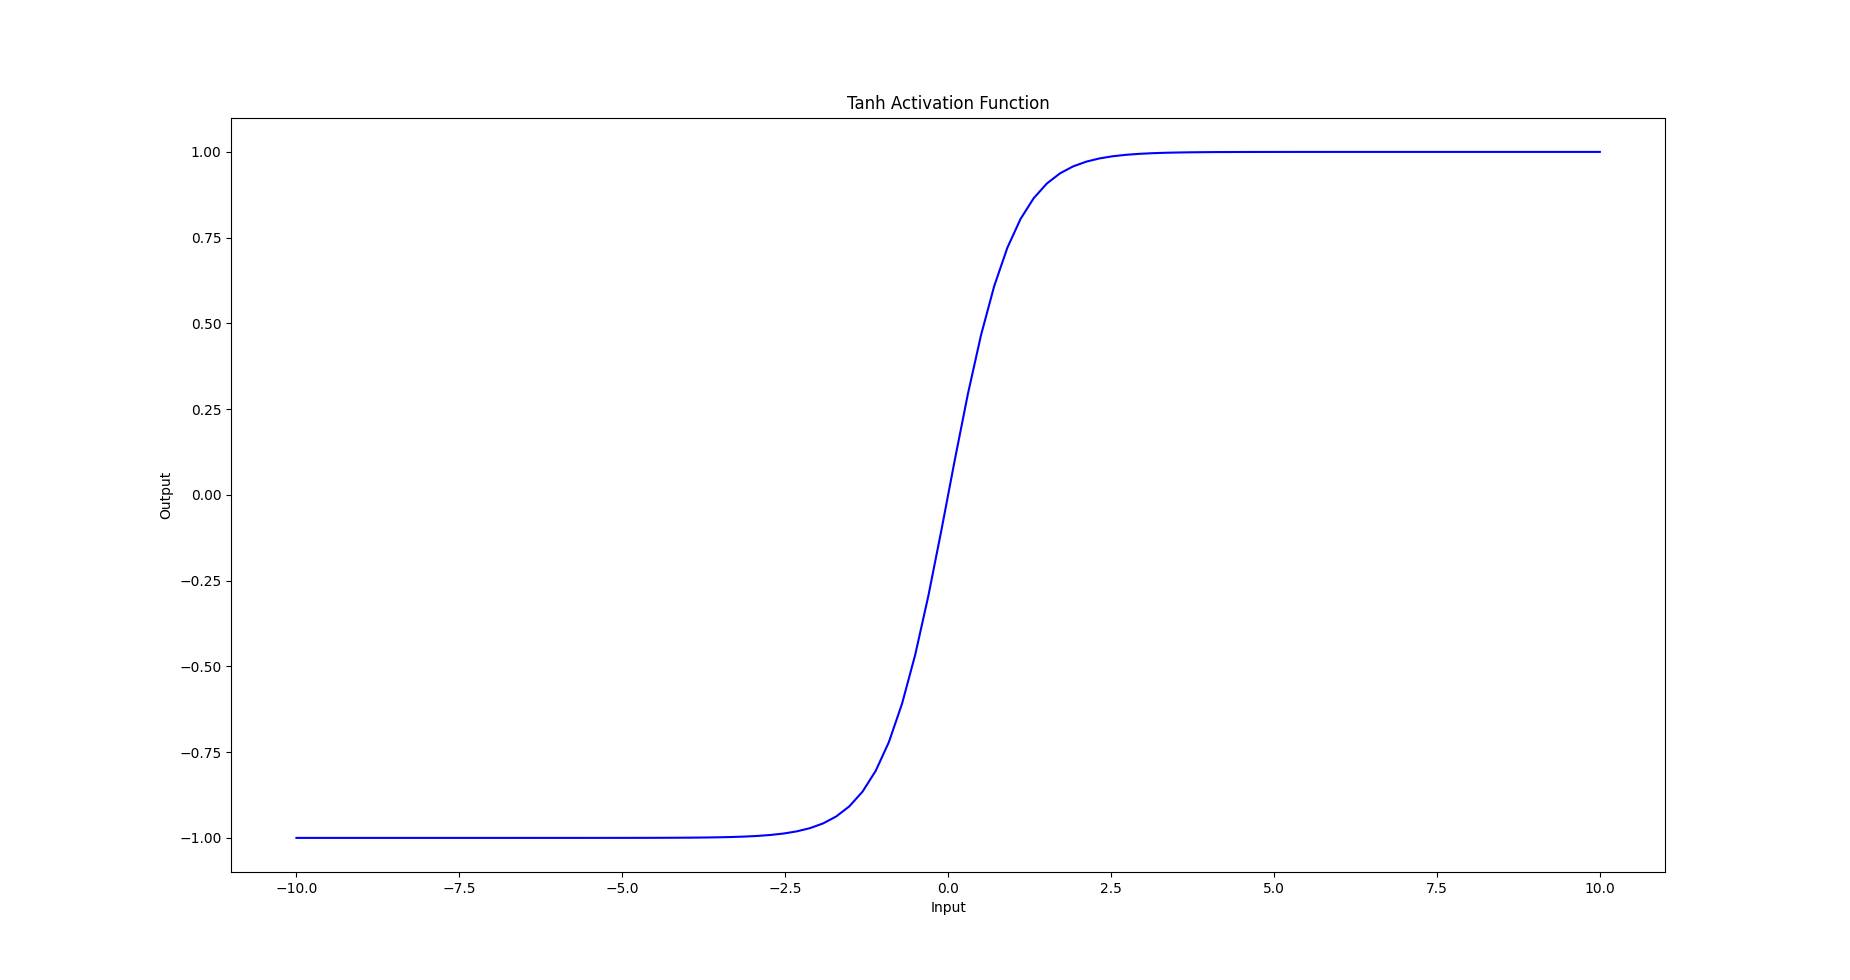
\includegraphics[width=8cm]{chapters/chapter2/tanh}
		\caption{Tanh activation}
		\label{tanh}
	\end{figure}
\end{itemize} 

Output layer has no activation function. it is connected to the loss function. The most used loss functions are:
\begin{itemize}
	\item Mean Absolute Error(MAE)
	\begin{equation}
		\text{MAE}(y,\hat{y}) = \frac{1}{N}\sum^N_i \left|y_i-\hat{y}_i\right|
	\end{equation}
	
	\item Mean Squared Error(MSE)
	\begin{equation}
		\text{MSE}(y,\hat{y}) = \frac{1}{N}\sum^N_i \left(y_i-\hat{y}_i\right)^2
	\end{equation}
	
	\item HuberLoss
	\begin{equation}
		\text{HuberLoss}(y,\hat{y};\delta) = \left\{\begin{matrix}
			\frac{1}{2}(y - \hat{y})^{2} & if \left | (y - \hat{y})  \right | < \delta\\
			\delta ((y - \hat{y}) - \frac1 2 \delta) & otherwise
		\end{matrix}\right.
	\end{equation}
	
\end{itemize}.

\subsection{Optimizers}
To do backpropagation we need an optimizer to update our learnable parameters. The easiest optimizer is stochastic gradient descent.
\begin{equation}
	\mathbf{W}^{(i+1)} =\mathbf{W}^{(i)}-\mu \frac{\partial Loss(z)}{\partial \mathbf{W}^{(i)}}
\end{equation}
There are more better one and for our use case we will use AdamW\cite{adamW}.

\subsection{Backpropagation of Neural Models}
After forward pass and calculated loss, we need to do just next steps Backward pass and optimization step.\\In backward pass we are computing the gradients of our learnable parameters to use it for the optimization of the model.\\
For example we will use stochstic gradient descent(SGD)
\begin{eqnarray}
	\mathbf{W}_{i+1} = \mathbf{W}_i - \gamma\cdot \frac{\partial Loss(z)}{\partial \mathbf{W}_i }\\
	\mathbf{b}_{i+1} = \mathbf{b}_i - \gamma\cdot \frac{\partial Loss(z)}{\partial \mathbf{b}_i }
\end{eqnarray} where $\gamma$ is a learning rate and one layered MLP
without bias $\mathbf{b}$.
\begin{eqnarray}
	\mathbf{z}_1 = \mathbf{W_0}\mathbf{y_0}\\ 
	\mathbf{y}_1 = \sigma(\mathbf{z}_1)\\
	\text{Loss}(y_1,\hat{y}) = \text{MSE}(y_1,\hat{y})
\end{eqnarray}
The obtaining the gradients of the weights is called backpropagation because for its calculation we need to apply chain rule for derivation.
\begin{equation}
\frac{\partial Loss(z)}{\partial \mathbf{W}_0}= \frac{\partial Loss(z)}{\partial \mathbf{y}_1} \cdot\frac{\partial \mathbf{y}_1}{\partial \mathbf{z}_1}\cdot	\frac{\partial \mathbf{z}_1}{\partial \mathbf{W}_0}
\end{equation}
Recurrent neural networks often fall as a victim of gradient vanishing or gradient exploding. In this manner the models doesn’t learn because the derivations calculated through backpropogation are to small or to big. It is important that gradients slowly decrease trough learning that whole model can generalize the data.

\chapter{Datasets}
Now we consider the study case of the datasets:
\begin{itemize}
	\item  N body problem
	\item Two body problem
	\item Threebody problem
	\item N pendelum
\end{itemize}
First we will mathematically describe the system and later we will explain how to prepare and create trajectories corresponding to their starting point/initial value. 


\section{Oscilator}
As we already shown the oscillator solution, we could show solution of the oscilator trough hamiltonian equations.
For this we will use Kinetic Energy $T =\frac{1}{2}mv^2$ and Potentional energy $U = \frac{1}{2}kx^2$. Using the momentum $p = mv$ we can rewrite our 
Kinetic energy as  $T =\frac{1}{2m}p^2$.\\
Using Hamiltonian Energy definition we obtain following equation: 
\begin{equation}
	\mathcal{H} = \frac{1}{2m}p^2 + \frac{1}{2}kx^2
\end{equation} 
This case is trivial.
We could get $\dot{x}$ and $\dot{p}$ trough hamiltonian equations $\dot{q} = \frac{\partial H}{\partial p}$ and $\dot{p} = - \frac{\partial H}{\partial q}$,
or we could compare Hamiltonian with elipse formula
\begin{equation}
	1 = \frac{x^2}{a^2} + \frac{y^2}{b^2},
\end{equation} and set the components in parametric equation\begin{equation}
(x,y) = (a\cos(\phi),b\sin(\phi)) \rightarrow(p,q) = \left(\sqrt{2Hm}\cos(\phi),\sqrt{\frac{2H}{k}}\sin(\phi)\right)
\end{equation} of the ellipse.\\ This equation represents kinematics of the oscilator. To find periodicity let say that $\phi = \omega t + \Phi $ and we know that the $p = mx$, with this equation we can calculate $\omega$.
\begin{eqnarray}
	p &=& m\dot{x} =\sqrt{2Hm}\cos(\omega t + \Phi), \\
	\dot{x} &=& \sqrt{\frac{2H}{m}}\cos(\omega t + \Phi),\\
		x &=& \int \sqrt{\frac{2H}{m}}\cos(\omega t + \Phi)dt = \frac{1}{\omega}\sqrt{\frac{2H}{m}}\sin(\omega t + \Phi) = \sqrt{\frac{2H}{k}} \sin(\omega t + \Phi),\\
	\omega &=& \sqrt{\frac{k}{m}} 
\end{eqnarray}  




The oscliator has harmonic, periodic movement which means that after some time $T$ the movement will be repeated $x(t_0) = x(t_N)$. With that property we can calculate the period over circle circumference:
\begin{equation}
	T = \frac{2\pi}{\omega}
\end{equation}

With this we can create a dataset within the program code. For coding we used framework $\texttt{pytorch}$ to calculate this dataset numerically.\\
For the obtain the solution of ODE we used package \texttt{torchdiffeq}\cite{torchdiffeq} to solve numerical equation with dopri5 method, which is most accurate method for solving ODEs.\\
To create unique trajectories for the dataset we just need to specify energy region.


\section{N-body problem}
N-body problem is most complex problem in physics. It describes a movement of bodies in the free space. There are no conditions and there are multitude of solutions. This problem is even a topic in quantum theory.\\ We will just observe an compute real trajectories of this problem.\\ 
In Newtonian formulation the N-body problem is
\begin{equation}
m_i\ddot{\mathbf{x}}_i = -\sum_{i\neq j, j=1}^nG\frac{m_im_j(\mathbf{x}_i-\mathbf{x}_j)}{||\mathbf{x}_i-\mathbf{x}_j||^3}
\end{equation} 
and its Hamiltonian:
\begin{equation}
	\mathcal{H} =\sum_i^n \frac{1}{2m_i}||\mathbf{p}_i||^2 - \sum_{1<i,j<n,i\neq j}\frac{Gm_im_j}{||\mathbf{x}_i-\mathbf{x}_j||}
\end{equation} 
for $i \in[1,n].$
N body problem is very complex problem because we need to achieve a conservative property of the Hamiltonian in the system\\
The biggest issue in this dataset are the crashes between the bodies.
This can be resolved with simple trick adding the $\epsilon$ to fix maximal potentional energy
\begin{equation}
	- \sum_{1<i,j<n,i\neq j}\frac{Gm_im_j}{||\mathbf{x}_i-\mathbf{x}_j||+\epsilon}.
\end{equation}
We secured that the value in the dominator never reaches 0. This is important because we use numerical solvers to create trajectories. If we have energy which achieves very big difference in values between two time steps, our solution will be inaccurate.  For calculation of such trajectories we are forced not to calculate over the Hamiltonian equations, but to calculate the trajectories using acceleration, velocity and position of the bodies trough some symplectic numerical methods. The code base for computation of the dataset we borrowed from \cite{nb}. In the code we introduced changes like solver, we used leapfrog and beeman method for calculating the trajectories.\\
To create the dataset we carefully chosed those constalations which are in fixed domain and the hamiltonian looks conservative. This conservative property is observable trough mean and standard deviation of the Hamiltonian Energy 
\subsection{Symplectic numerical methods to solve N-body problem}
Symplectic numerical methods are designed for numerical solution of Hamilton Equations. It posses conserved quality to approximate the Total Energy the Hamiltonian.\\
They have two forms. One in canonical coordinates($q$,$p$) and in langrangian coordinates($x$,$v$,$a$). Most used ones are in langrangian form and we will use it to create trajectory for N-body problem.\\
For the N-body problem we used two numerical solvers. In first step we used velocity verlet
\begin{eqnarray}
	\mathbf{x}_{i+1} &=& \mathbf{x}_i + h\mathbf{v}_i + \mathbf{a}_i\frac{h^2}{2} \\
	\mathbf{v}_{i+1}&=&\mathbf{v}_i + (\mathbf{a}_i +\mathbf{a}_{i+1})\frac{h}{2}
\end{eqnarray} and
for the next steps with timestep $h$ we used more stable beeman method
\begin{eqnarray}
	\mathbf{x}_{i+1} &=& \mathbf{x}_i + h\mathbf{v}_i + \frac{h^2}{6}(4\mathbf{a}_{i}-\mathbf{a}_{i-1})\\
	\mathbf{v}_{i+1}&=&\mathbf{v}_i + \frac{h}{6}(2\mathbf{a}_{i+1} + 5\mathbf{a}_i-\mathbf{a}_{i+1}).
\end{eqnarray}
This needed to be done because the beeman method needs acceleration of the next and previous step to be calculated. We used langragian coordinates because it is most easiest way to create trajectories.
In canonical coordinates we need more formulas like for hamiltonian energy and its derivation. In thi way we can very fast calculate the trajecories of nbody problem. The dataset is fully adjustable. We can adjust gravity constant and masses how we like. As proof of concept we used $G=1$ and $m_i=1$.  
\subsection{Twobody problem}
Twobody problem is one of the most easiest dataset which could be created from N-body problem. It has one trivial solution which is binary star movement which is periodic.
Two stars trough their movement maintain constant distance $r$ and their center of mass $\mathbf{p}_m$ is static at the origin.\\
The newtonian form of twobody Problem is written as
\begin{eqnarray}
	m_1\ddot{\mathbf{q}}_1 = -G\frac{m_1m_2(\mathbf{q}_1-\mathbf{q}_2)}{||\mathbf{q}_1-\mathbf{q}_2||^3}\\
	m_2\ddot{\mathbf{q}}_2 = -G\frac{m_1m_2(\mathbf{q}_2-\mathbf{q}_1)}{||\mathbf{q}_2-\mathbf{q}_1||^3}
\end{eqnarray}
From those equations we can get a statement about third newton law:
\begin{equation}
	m_1\ddot{\mathbf{q}}_1 -m_2\ddot{\mathbf{q}}_2 = 0 = \mathbf{F}_{ij} - \mathbf{F}_{ji}
\end{equation}
and its hamiltonian
\begin{equation}
\mathcal{H} = \frac{||\mathbf{p}_1||}{2m_1} +\frac{||\mathbf{p}_2||}{2m_2} - G\frac{m_1m_2}{||\mathbf{q}_1 - \mathbf{q}_2||}.
\end{equation}
We said that we have static center mass point. center mass point is obtained using following formula
\begin{equation}
	\mathbf{q}_m = \frac{1}{m_1+m_2}(m_1\mathbf{q_1} + m_2\mathbf{q_2}).
\end{equation}
If we set the center mass point in origin the equation simplifies nd we get one about velocity
\begin{eqnarray}
	m_1\mathbf{q_1} + m_2\mathbf{q_2} = 0,\\
	m_1\dot{\mathbf{q}}_1 + m_2\dot{\mathbf{q}}_2 = \mathbf{p}_1 +\mathbf{p}_2 = 0.
\end{eqnarray}
From now on we will write $\mathbf{p} =\mathbf{p}_1 = -\mathbf{p}_2$.
Lets make some formulas about distance
\begin{eqnarray}
	\mathbf{q}_2 = \frac{m_1}{m_2}\mathbf{q}_2,\\
	||\mathbf{q}_2|| =^{\mathbf{q}_m=0} \frac{m_1}{m_2}||\mathbf{q}_1||,\\ 
	r_2 =\frac{m_1}{m_2}r_1.
\end{eqnarray}
With this we got interesting property
\begin{equation}
	\frac{r_1}{r_2} =\frac{m_2}{m_1}. 
\end{equation}
This can be used to calculate constant distance between the bodies
\begin{equation}
	r=r_1\left(1 + \frac{m_1}{m_2}\right).
\end{equation}

With those equations we can simplify hamiltonian \begin{equation}
	\mathcal{H}= ||\mathbf{p}||^2\left(\frac{1}{m_1}+\frac{1}{m_2}\right) - G\frac{m_1m_2}{r}.
\end{equation}
Still to make a dataset with twobody trajectories we need a period $T$. Let assume that our solution as describe is radial. the bodies moves on a circular path
\begin{eqnarray}
	\mathbf{q}_1 = r_1
	\begin{bmatrix}
		\cos(\Phi)\\
		\sin(\Phi)
	\end{bmatrix},\\
\mathbf{q}_2 = r_2
\begin{bmatrix}
	\cos(\Phi+ \pi)\\
	\sin(\Phi+ \pi)
\end{bmatrix}.
\end{eqnarray}
The momentum is tangential in dependency of orientation of position
\begin{eqnarray}
	\mathbf{p}_1 = ||\mathbf{p}||
	\begin{bmatrix}
		\sin(\Phi)\\
		-\cos(\Phi)
	\end{bmatrix}\\
	\mathbf{p}_2 = ||\mathbf{p}||
	\begin{bmatrix}
		\sin(\Phi+ \pi)\\
		-\cos(\Phi+ \pi)
	\end{bmatrix}
\end{eqnarray} with $\Phi \in [0,2\pi] $.
Let say that $\Phi=\omega t$
and we want to find a period of movement.
With the equations
\begin{eqnarray}
	\dot{\mathbf{q}}_1 = r_1\omega
	\begin{bmatrix}
		\sin(\omega t)\\
		-\cos(\omega t)
	\end{bmatrix}\\ = \frac{\mathbf{p_1}}{m_1} = \frac{||\mathbf{p}||}{m_1}\begin{bmatrix}
	\sin(\omega t)\\
	-\cos(\omega t)
\end{bmatrix}\\
||\mathbf{p}|| = r_1m_1\omega,
\end{eqnarray}
we calculated the value of the momentum.
This momentum we can get from Physics and newton third law: if some body moves around some point in radial path, we can calculate a centripetal Force and this Force should be equal to Gravitational Force
\begin{equation}
	F_c = \frac{||\mathbf{p}||^2}{m_1r_1} = \frac{Gm_1m_2}{r^2} = F_g.
\end{equation}
Substituting $||\mathbf{p}||$ we get $\omega$
\begin{equation}
	\omega = \frac{1}{r}\sqrt{G\frac{m_2}{r_1}}
\end{equation} and $T$
 \begin{equation}
 	T = \frac{2\pi}{\omega}.
 \end{equation}
In two body problem to create some diverse dataset but with equivalent bodies we vary the distance between the bodies. We need to be careful because with grater distance $r$ the period $T$ will be longer.\\
The mathematical formulation of the solution which is used for code is taken from hamiltonian equations
\begin{equation}
	\dot{\mathbf{x}} = J\frac{\partial H}{\partial \mathbf{x}}(\mathbf{x})=
\begin{bmatrix}
	0 & 0 & 0 & 0 & \frac{1}{m_1} & 0\\
	0 & 0 & 0 & 0 & 0 & \frac{1}{m_1}\\
	0 & 0 & 0 & 0 & -\frac{1}{m_2} & 0\\
	0 & 0 & 0 & 0 & 0 & -\frac{1}{m_2}\\
	-\mu_{1,2} & 0 & \mu_{1,2} & 0 & 0 & 0 \\
	0 & -\mu_{1,2} & 0 & \mu_{1,2} & 0 & 0 \\
\end{bmatrix}
\begin{bmatrix}
	q_{1x}\\
	q_{1y}\\
	q_{2x}\\
	q_{2y}\\
	p_x\\
	p_y
\end{bmatrix} 
\end{equation} where $\mu_{ij}=\frac{Gm_im_j}{r^3}.$
We used Dopri5 to create the trajectories. To diversify our dataset we suggest to define the distance region and pick randomly the distance between the bodies. The mases should be the same.

\subsection{Three body problem}
Three body problem is from formulation similar to two body problem, but finding the periodic solutions is very complex task. Fortunatly the M. Šuvlakov and V. Dmitrašinović have found many of the initial values to create periodic three body trajectory in 2D space and made data public over the website for everyone to use.\cite{papthreebody}\cite{web}. It is important to mention that they made it to mathematical problem which means that the parameters like the gravitational constant $G$ and all masses $m$ are set to 1.
Even today there are scientists which are documenting initial values for more periodic solutions \cite{hudomal2015new}.
Having those conditions we need just Hamiltonian equations which are easy to obtain. 

Obtaining the formula for straight-forward calculation the trajectories of the threebody problem we need to define a function
\begin{equation}
	\boldsymbol{\Xi}(\mathbf{q}_i,\mathbf{q}_j)=\boldsymbol{\Xi}_{i,j}=\frac{Gm_im_j}{||(\mathbf{q}_i-\mathbf{q}_j)||^3}.
\end{equation}
In following consider $\mathbf{m_i^{⁻1}}=\text{diag}(\frac{1}{m_i},\frac{1}{m_i})$ and coordinates are two dimensional.
\begin{equation}
	\dot{\mathbf{x}} = 
	\begin{bmatrix}
		0 & 0 & 0 & \mathbf{m_1^{⁻1}} & 0 & 0\\
		0 & 0 & 0 & 0 & \mathbf{m_2^{⁻1}} & 0\\
		0 & 0 & 0 & 0 & 0 & \mathbf{m_3^{⁻1}}\\
		-(\boldsymbol{\Xi}_{1,2}+\boldsymbol{\Xi}_{1,3}) & \boldsymbol{\Xi}_{1,2} & \boldsymbol{\Xi}_{1,3} & 0 & 0 & 0\\
		\boldsymbol{\Xi}_{1,2} & -(\boldsymbol{\Xi}_{1,2}+\boldsymbol{\Xi}_{2,3}) & \boldsymbol{\Xi}_{2,3} & 0 & 0 & 0\\
		\boldsymbol{\Xi}_{1,3} & \boldsymbol{\Xi}_{2,3} & -(\boldsymbol{\Xi}_{1,3}+\boldsymbol{\Xi}_{2,3}) & 0 & 0 & 0\\
	\end{bmatrix}
	\begin{bmatrix}
		\mathbf{q}_1\\
		\mathbf{q}_2\\
		\mathbf{q}_3\\
		\mathbf{p}_1\\
		\mathbf{p}_2\\
		\mathbf{p}_3
	\end{bmatrix}
\end{equation}
To diversify our dataset we found that
the three-body problem has two interesting properties due its defined potentional energy. Their potential energy is defined over gravitational force between the bodies. In another words we can translate the trajectories together in space and rotate it without changing the hamiltonian value. Let us prove this over Hamiltonian Energy
\begin{equation}
	\mathcal{H} = \frac{||\mathbf{p}_1||^2}{2m_1} +\frac{||\mathbf{p}_2||^2}{2m_2}+\frac{||\mathbf{p}_3||^2}{2m_3} - G\frac{m_1m_2}{||\mathbf{q}_1 - \mathbf{q}_2||}-G\frac{m_2m_3}{||\mathbf{q}_2 - \mathbf{q}_3||}-G\frac{m_1m_3}{||\mathbf{q}_1 - \mathbf{q}_3||}. 
\end{equation}-
\begin{itemize}
	\item Translation:\\
	Lets define $\mathbf{q}_i = \lim_{\mathbf{q}_t\rightarrow \mathbf{0}}(\mathbf{q}_i + \mathbf{q}_t)$ where $\mathbf{q}_t$ is translation vector. When we substitute $\mathbf{q}_i$. The hamiltoinian acts as follows
	\begin{eqnarray*}
		\mathcal{H} &=& \frac{||\mathbf{p}_1||^2}{2m_1} +\frac{||\mathbf{p}_2||^2}{2m_2}+\frac{||\mathbf{p}_3||^2 }{2m_3}\\
		& & - \lim_{\mathbf{q}_t\rightarrow \mathbf{0}}G\frac{m_1m_2}{||\mathbf{q}_1+ \mathbf{q}_t  - (\mathbf{q}_2+ \mathbf{q}_t) ||}-\lim_{\mathbf{q}_t\rightarrow \mathbf{0}}G\frac{m_2m_3}{||\mathbf{q}_2 + \mathbf{q}_t - (\mathbf{q}_3+ \mathbf{q}_t) ||}\\
		& &-\lim_{\mathbf{q}_t\rightarrow \mathbf{0}}G\frac{m_1m_3}{||\mathbf{q}_1+ \mathbf{q}_t  - (\mathbf{q}_3+ \mathbf{q}_t) ||}\\
		&=& \frac{||\mathbf{p}_1||}{2m_1} +\frac{||\mathbf{p}_2||}{2m_2}+\frac{||\mathbf{p}_3||}{2m_3}\\ & &-  G\frac{m_1m_2}{||\mathbf{q}_1 - \mathbf{q}_2 +(\mathbf{q}_t-\mathbf{q}_t) ||}-G\frac{m_2m_3}{||\mathbf{q}_2 - \mathbf{q}_3 +(\mathbf{q}_t-\mathbf{q}_t)||}\\
		& &-G\frac{m_1m_3}{||\mathbf{q}_1 - \mathbf{q}_3+(\mathbf{q}_t-\mathbf{q}_t)||}\\
		& = & \frac{||\mathbf{p}_1||}{2m_1} +\frac{||\mathbf{p}_2||}{2m_2}+\frac{||\mathbf{p}_3||}{2m_3} - G\frac{m_1m_2}{||\mathbf{q}_1 - \mathbf{q}_2||}-G\frac{m_2m_3}{||\mathbf{q}_2 - \mathbf{q}_3||}-G\frac{m_1m_3}{||\mathbf{q}_1 - \mathbf{q}_3||} 
	\end{eqnarray*}
	\item Rotation:
	Lets define $\mathbf{q}_i = r_i \begin{bmatrix}
		\cos(\beta + \alpha)\\
		\sin(\beta + \alpha)\\
		\end{bmatrix}$ and $\mathbf{p}_i = p_i \begin{bmatrix}
		-\sin(\beta + \alpha)\\
		\cos(\beta + \alpha)\\
		\end{bmatrix}$\\
	 where $\beta \in (0,2\pi]$ but it is defined and $\alpha \in (0,2\pi] $  which is free parameter.\\
	Let substitute this in Hamiltonian
	\begin{eqnarray*}
		\mathcal{H} &=& \frac{\left|\left| p_1 \begin{bmatrix}
				-\sin(\beta + \alpha)\\
				\cos(\beta + \alpha)\\
			\end{bmatrix}\right|\right|^2}{2m_1} +\frac{\left|\left| p_2 \begin{bmatrix}
			-\sin(\beta + \alpha)\\
			\cos(\beta + \alpha)\\
		\end{bmatrix}\right|\right|^2}{2m_2}+\frac{\left|\left| p_3 \begin{bmatrix}
		-\sin(\beta + \alpha)\\
		\cos(\beta + \alpha)\\
	\end{bmatrix}\right|\right|^2}{2m_3}\\& & - G\frac{m_1m_2}{\left|\left|r_1 \begin{bmatrix}
	\cos(\beta + \alpha)\\
	\sin(\beta + \alpha)\\
\end{bmatrix} - r_2 \begin{bmatrix}
\cos(\beta + \alpha)\\
\sin(\beta + \alpha)\\
\end{bmatrix}\right|\right|}\\
& &-G\frac{m_2m_3}{\left|\left|r_2 \begin{bmatrix}
\cos(\beta + \alpha)\\
\sin(\beta + \alpha)\\
\end{bmatrix} - r_3 \begin{bmatrix}
\cos(\beta + \alpha)\\
\sin(\beta + \alpha)\\
\end{bmatrix}\right|\right|}\\
& &-G\frac{m_1m_3}{\left|\left|r_1 \begin{bmatrix}
\cos(\beta + \alpha)\\
\sin(\beta + \alpha)\\
\end{bmatrix} - r_3 \begin{bmatrix}
\cos(\beta + \alpha)\\
\sin(\beta + \alpha)\\
\end{bmatrix}\right|\right|} 
\end{eqnarray*}
From trigonometry we know that $\cos(\phi)^2 + \sin(\phi)^2= 1$.\\
From that we get $\left|\left|\begin{bmatrix}
	\cos(\beta + \alpha)\\
	\sin(\beta + \alpha)\\
\end{bmatrix}\right|\right| =\left|\left|\begin{bmatrix}
\cos(\beta)\\
\sin(\beta)\\
\end{bmatrix}\right|\right|= 1$.\\
Applying this theorem we get 
\begin{equation}
	\mathcal{H} = \frac{p_1^2}{2m_1} +\frac{p_2^2}{2m_2}+\frac{p_3^2}{2m_3} - G\frac{m_1m_2}{|r_1 - r_2|}-G\frac{m_2m_3}{|r_2 - r_3|}-G\frac{m_1m_3}{|r_1 - r_3|}
\end{equation} which is equivalent to the previous definition.
\end{itemize}
For the dataset creation we wanted that our trajectory mass middle point is fixed. We needed only rotation around it.
For such rotation we used formula for such transformation
\begin{equation}
	\hat{\mathbf{q}} = 
	\begin{bmatrix}
		1 & 0 & 0 & x_m\\
		0 & 1 & 0 & y_m\\
		0 & 0 & 1 & z_m\\
		0 & 0 & 0 & 1
	\end{bmatrix}	
\begin{bmatrix}
	\cos(\alpha) & -\sin(\alpha) & 0 & 0\\
	\sin(\alpha) & \cos(\alpha) & 0 & 0\\
	0 & 0 & 1 & 0\\
	0 & 0 & 0 & 1
\end{bmatrix}
\begin{bmatrix}
	1 & 0 & 0 & -x_m\\
	0 & 1 & 0 & -y_m\\
	0 & 0 & 1 & -z_m\\
	0 & 0 & 0 & 1
\end{bmatrix}
\begin{bmatrix}
	x_q\\
	y_q\\
	z_q\\
	1
\end{bmatrix},
\end{equation} which for two dimensional cases can be rewritten as
\begin{equation}
	\hat{\mathbf{q}} = \mathbf{R}\mathbf{q} - \mathbf{R}\mathbf{q}_m + \mathbf{q}_m,
\end{equation} where $\mathbf{R}=\begin{bmatrix}
\cos(\alpha) & -\sin(\alpha)\\
\sin(\alpha) & \cos(\alpha)\\
\end{bmatrix}$.

	


 
 \section{N Pendulum}
 The N Pendelum is straight forward model.
 To make it in canocnical coordinates which are angles of the joints, still we need to define Kinematic of the model.
 \begin{eqnarray}
 	x_i = \sum_i^n l_i\sin(\Theta_i)\\
 	y_i = -\sum_i^n l_i\cos(\Theta_i)
 \end{eqnarray}
Their temporal derivations are:
\begin{eqnarray}
\dot{x}_i = \sum_i^n \dot{\Theta}_i l_i\cos(\Theta_i)\\
	\dot{y}_i = \sum_i^n \dot{\Theta}_i l_i\sin(\Theta_i)
 \end{eqnarray}
From this kinematic model we just calculated the Hamiltonian and proceed with autodifferentiaion from pytorch framework to calculate the values of hamiltonian equations
\begin{eqnarray}
	\mathcal{H} = \frac{1}{2}\sum_i^n m_i (\dot{x}_i^2 + \dot{y}_i^2) + \sum_i^n m_ig_iy_i. 
\end{eqnarray}
We set a canonical coordinates $(\Theta, p_{\Theta})$ and we can calculate $p_{\Theta} = \frac{\partial H}{\partial \dot{\Theta}}$.
Making the Hamiltonan only dependent on $\Theta$ and $p_{\Theta}$ we can get hamiltonian equations:
\begin{eqnarray}
	\dot{\Theta_i} = \frac{\partial \mathcal{H}}{\partial p_{\Theta_i}}\\
	\dot{p_{\Theta_i}} = -\frac{\partial \mathcal{H}}{\partial \Theta}
\end{eqnarray}
This was done using auto-differentiation and we managed to create dataset models for (1,2,3,4) degrees of freedom, which offers very accurate hamiltonian values in the dataset. 
The dataset need fixed inital values like  $\Theta \in [-\frac{\pi}{6},\frac{\pi}{6}]$ and starting $p_{\Theta_i} = 0 $.\\
We can create a dataset with observation. With interest to creating of 3D models as´ \texttt{urdf} files, we created the framework which trough python coding crates accurate urdf model, in our case $N$ Pendelum. This was used to create pendulum with $N$  number of joints. This model was created for and  observed in \texttt{pybullet}\cite{pybullet}. From the use case we suggest if you are working with pendelums where $N<10$ please use the pytorch numerical technique, otherwise use \texttt{pybullet} observation. \texttt{Pybullet} can extract, almost in real-time, the movement and velocities of the pendelum. Only we need to calculate if Hamiltonian energy is stable enough for our experiments.\\ In the case that we didn't got any velocity for our dataset it is possible to obtain it over trajectory trough "euler trick"
\begin{equation}
	\mathbf{v}_i=\mathbf{f}(\mathbf{x}_i) = \frac{\mathbf{x}_{i+1}-\mathbf{x}_i}{h}.
\end{equation}
In Figure \ref{pyb} you can see the Pendelum in \texttt{Pybullet }simulation software

 \begin{figure}[h!]
 	\label{pend}
 	\centering
 	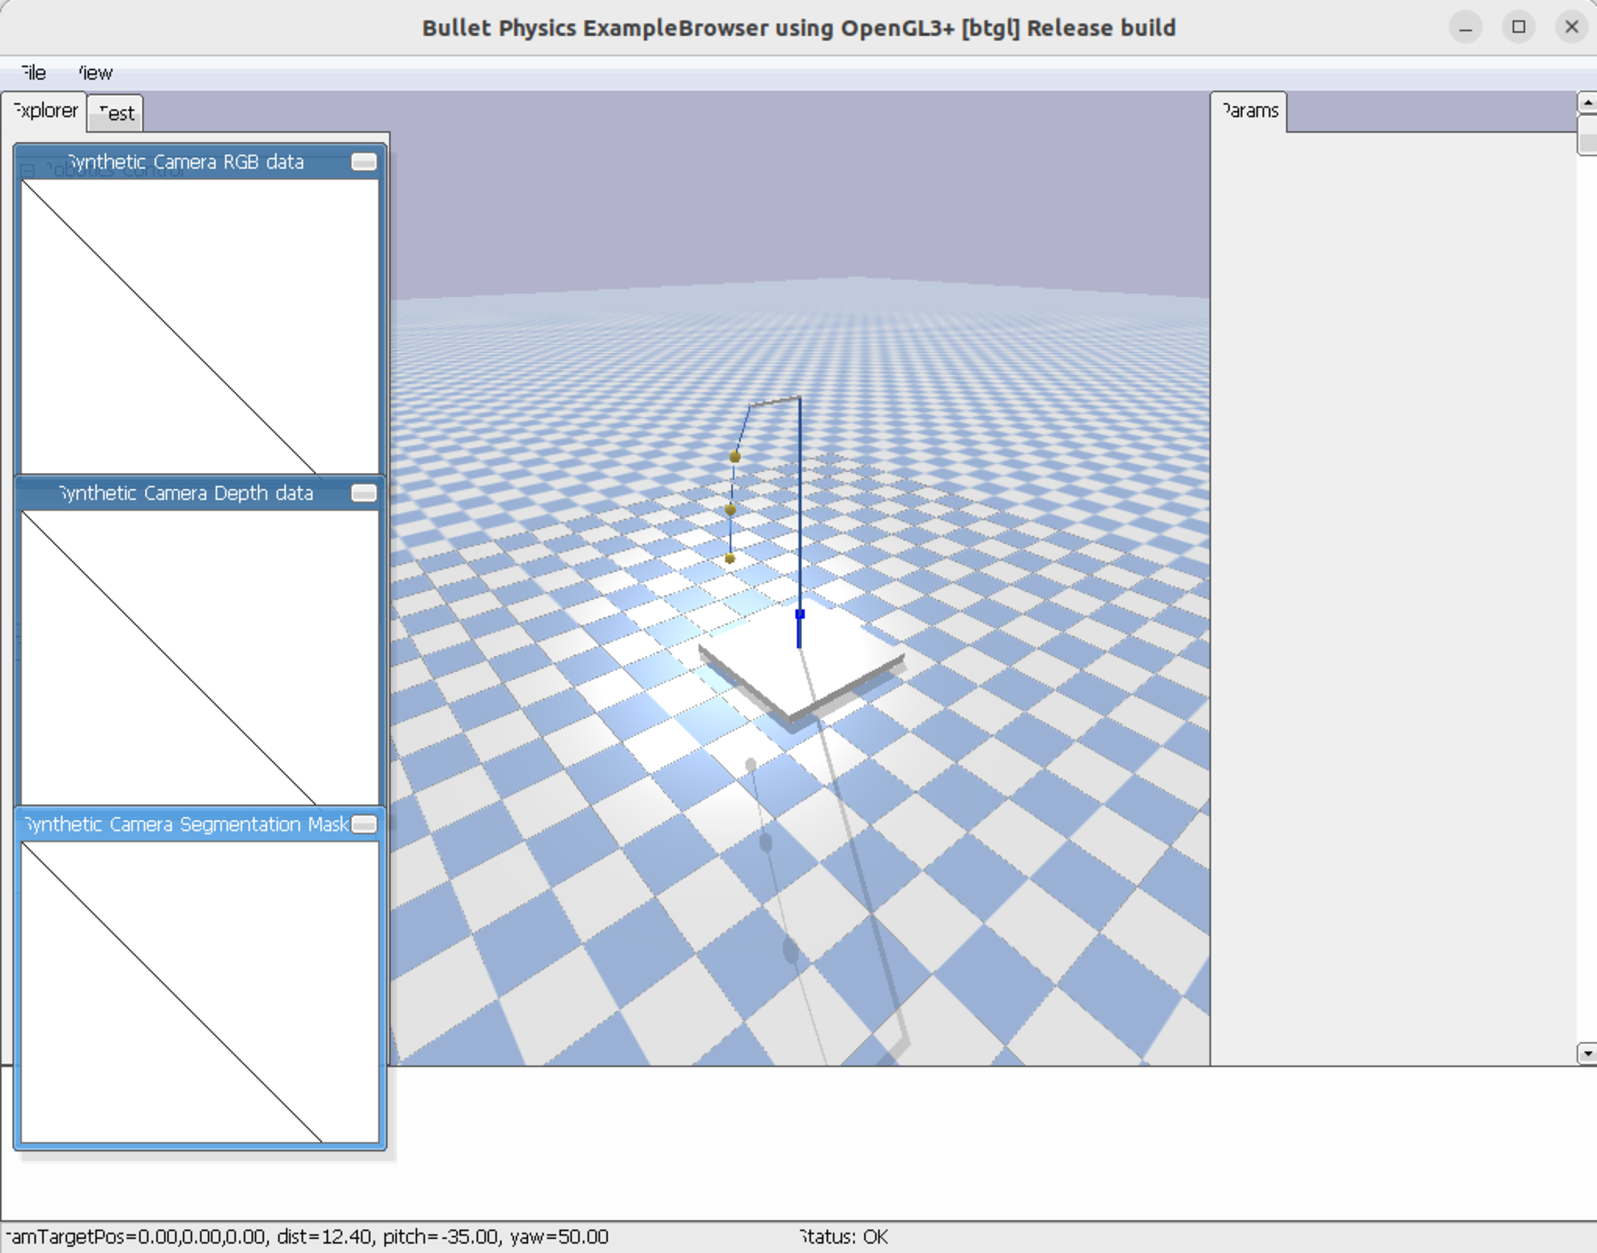
\includegraphics[width=10cm]{chapters/chapter3/pendulum.pdf}
 	\caption{Pendelum with 3 degrees of freedom in pybullet}
 	\label{pyb}
 \end{figure}




 
 


 


\chapter{Methods}
After previous chapters we should achieve basic understanding of neural network models and physics. Now we study state of the art methods which should capture hamiltonian model on studied datasets. 
\section{New paradigm - NeuralODE}
Neural ODE is very interesting and important concept for solving the Ordinary Differential Equations and training the neural networks with trajectory data.\\
The default situation is described as:
\begin{equation}
	\dot{\mathbf{x}}=\mathbf{f}(\mathbf{x},t|\Theta)
\end{equation}
Where $\mathbf{f}(\mathbf{x},t|\Theta) $ represents the multilayer perception which creates vector field.
This method has its history from residual networks where their feed-forward network looks like euler step
\begin{equation}
	\mathbf{h}^{(i+1)} = \mathbf{h}^{(i)} + \mathbf{f}(\mathbf{h}^{(i)}|\Theta)
\end{equation}

In the paper \cite{neuralODE} it is introduced a adjoint method  which solves problem with vanishing gradients.\\
This is achieved trough continuous backpropagation which is stated in the paper.
We can compare it 
\begin{center}
	\begin{tabular}{ c c|c }
		 & residual network & adjoint method \\ 
		 \hline
		$a_t$ or $a(t)$: & $\frac{\partial L}{\partial z}$ & $\frac{\partial L}{\partial z(t)}$ \\  
		forward-pass: & $z_{i+1} = z_t + hf(z_t)$ & $z(t+1) = z(t)+\int_t^{t+1}f(t)dt$\\
		backward-pass: &$a_t = a_{t+1}+ha_{t+1}\frac{\partial f(z_t)}{\partial z_t}$ & $a(t) = a(t+1)+\int_{t+1}^ta(t)\frac{\partial f(z(t))}{\partial z(z)}dt$\\
		gradients:  & $\frac{\partial L}{\partial \theta}=ha_{t+h}\frac{\partial f(z(t),\Theta)}{\partial \Theta}$ & $\frac{\partial L}{\partial \theta}=\int_t^{t+1}a(t)\frac{f(z(t),\Theta)}{\partial \Theta}$   
	\end{tabular}
\end{center}
For PINN models the adjoint method over framework \texttt{torchdiffeq} doesn't work properly because of the computed gradients which PINNs produce. In case of PINN models we suggest to use normal rollout with ode solver like RK4.


\section{Recurrent time steppers}
In chapter \ref{background}  we introduced recurrent models which are RNN and GRU.
Those models are very good at learning the time series data. To make it more physics informed we applied an euler method which it makes to time stepper models:
\begin{eqnarray}
	[\mathbf{v}_i, \mathbf{h}_{i+1}] = \text{RNN}(\mathbf{x}_i,\mathbf{h}_i) \text{  or  }  \text{GRU}(\mathbf{x}_i,\mathbf{h}_i)\\
	\mathbf{x}_{i+1} = \mathbf{x}_i + \mathbf{v}_i \cdot dt
\end{eqnarray}
We describe it this procedure as a rollout. 
This model has one big static parameter dependency which is fixed $dt$. We suggest to not to change this parameter after training. In Chapter Experimentation we will show the performance of RNN and GRU time stepper models. In the figure \ref{fig:rnn} we can see the architecture of the model.
\begin{figure}[h!]
	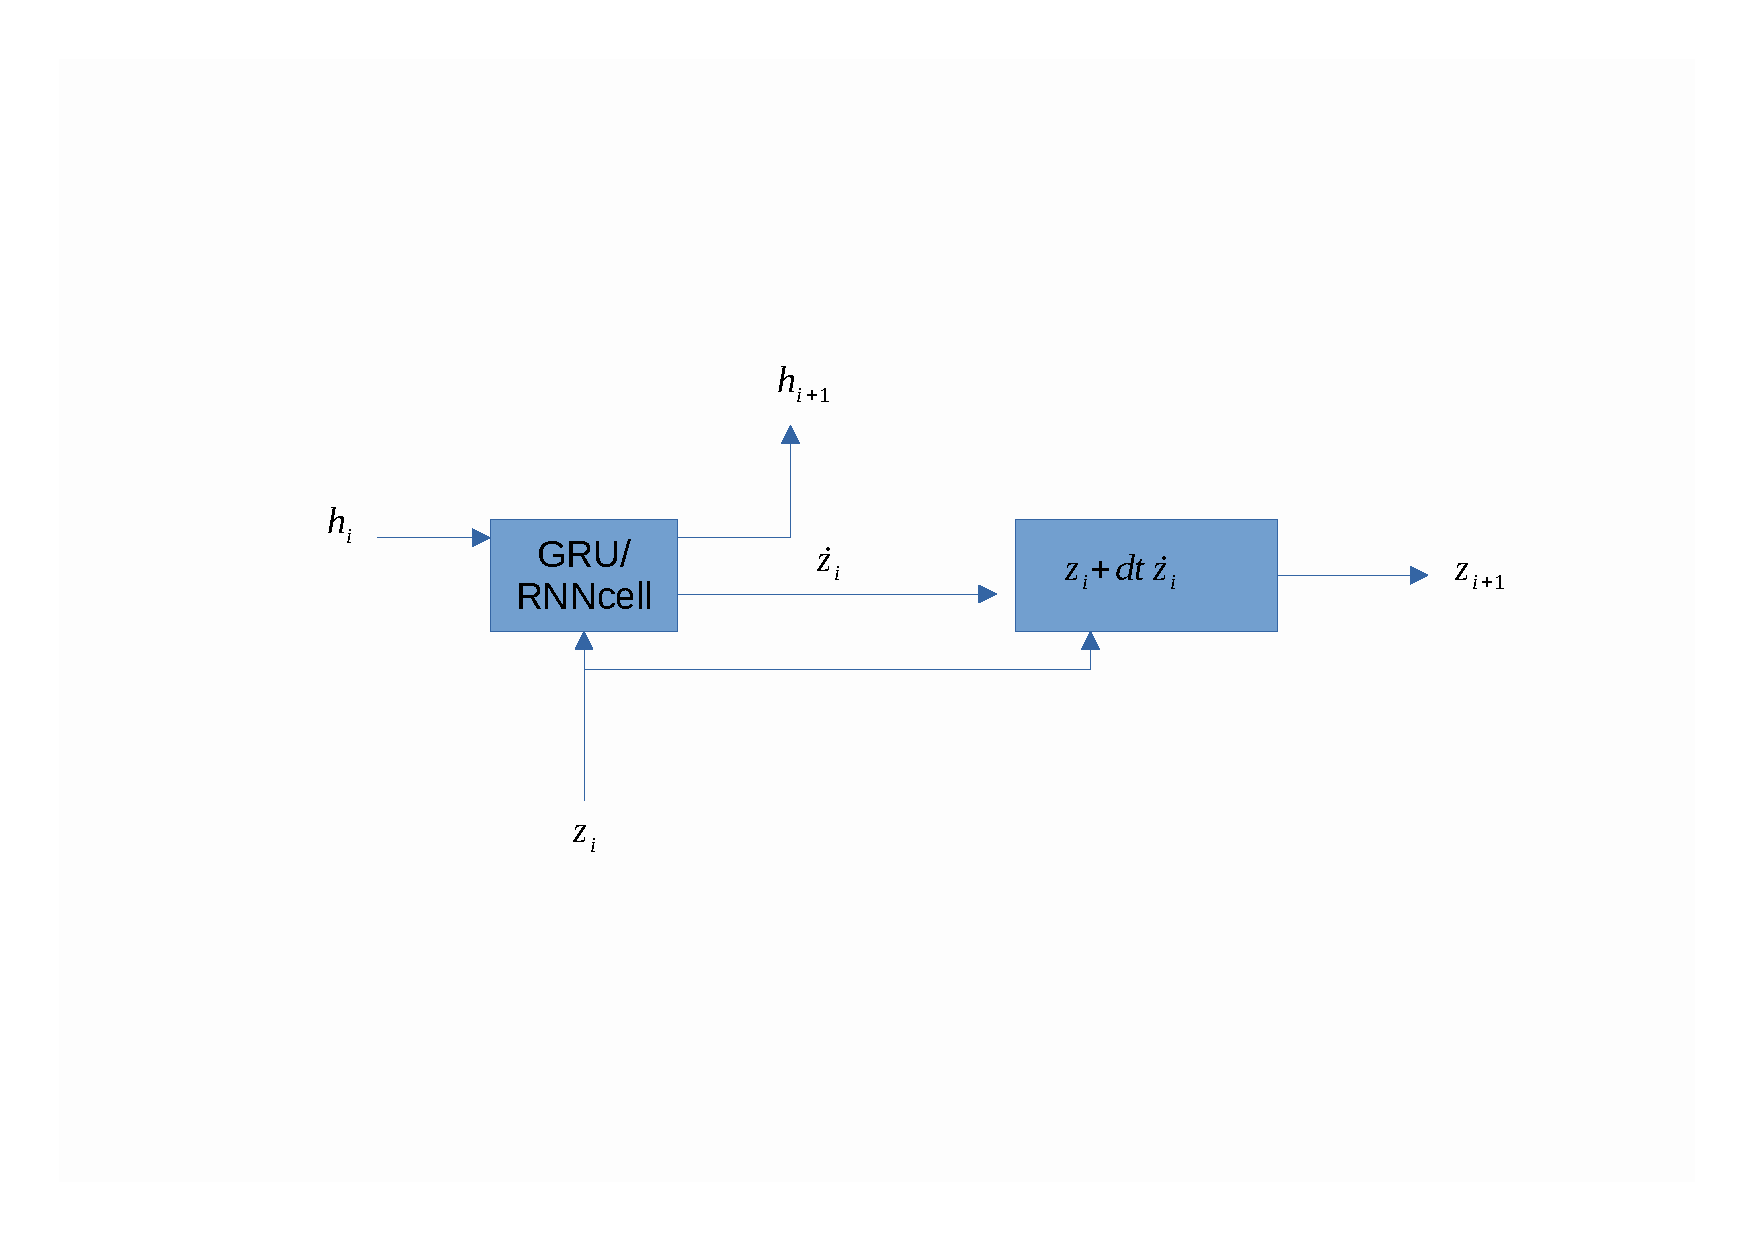
\includegraphics[width=15cm]{chapters/chapter4/RNN_stepper}
	
	\caption{Architecture of time-stepper model}
	\label{fig:rnn}
\end{figure}



\section{Hamiltonian Neural Network}
This model comes from the paper \cite{hnn} it is one of the physics informed models because it uses differentiation technique and applies the Hamiltonian equations. In this case the $\mathbf{x} = [\mathbf{q},\mathbf{p}]$ are canonical or natural coordinates(Cartesian space).
The forward pass looks like:
\begin{eqnarray}
	H_{\Theta} &=& \mathbf{f}(\mathbf{x}|\boldsymbol{\Theta})\\
	\frac{d\mathbf{x}}{dt}(\mathbf{x}) &=& \left[\frac{\partial H_{\Theta}}{\partial\mathbf{p}}(\mathbf{x}),-\frac{\partial H_{\Theta}}{\partial\mathbf{q}}(\mathbf{x})\right]^T
\end{eqnarray}
In the paper they train it only over the produced vectorfield.
For our experiments we made rollout part for the network to create trajectory. 
To make trajectory we use ODE solver
\begin{equation}
	\mathbf{x} = \text{odeint}\left(\frac{d\mathbf{x}}{dt},\mathbf{x}_0,t\right)
\end{equation} 
The odeint operator in this equation is a solver for ODEs like euler or RK4 method. In the experiments due the limitation of framework \texttt{pytorch} it is impossible to us ode solver based on adjoint method. We can observe it in the figure from chapter Introduction \ref{fig:hnn}.\\
\section{Graph Neural Network}
Graph neural Networks are very new neural architecture which is available today. It is used broadly in social sciences and in chemistry like generating new chemical compounds.\\
The main part of GNN is a graph $\mathbf{G}$. It is defined as a collection of vertices and edges $\mathbf{G}=\{\mathbf{V},\mathbf{E}\}$ where $\mathbf{V} = \{\mathbf{v}_1,...,\mathbf{v}_i,...,\mathbf{v}_n\}$ has $n$ vertices
and $\mathbf{E} = \{\mathbf{e}_1,...,\mathbf{e}_i,...,\mathbf{e}_m\}$
has $m$ edges.\\
The edge is connection between to nodes it can be directed(only one direction between the nodes) or undirected(both direction between the nodes). This is very important because the graphs has many properties which we can use building it as Graph Neural Model.\\
This connectivity can be represented with adjacency matrix $\mathbf{A}$.
Adjacency matrix is denoted as $\mathbf{A}\in \{0,1\}^{n x n}$ 
\begin{equation}
\mathbf{A}_{ij} =	\left\{\begin{matrix}
		1 & if (\mathbf{v}_i , \mathbf{v}_j)\in\mathcal{E}\\
		0 & otherwise
	\end{matrix}\right.
\end{equation}

Most important property of graphs is creating the normailzed Laplacian matrix. This is foundation of the idea about graph neural networks and it is defined as:
\begin{equation}
	\mathbf{L}= \mathbf{I} - \mathbf{D}^{\frac{1}{2}}\mathbf{A}\mathbf{D}^{\frac{1}{2}} 
\end{equation} where $\mathbf{D}$ is degree matrix. Degree of a node is the number of nodes that are adjecent to the node in question. This matrix has only diagonal elements.\\
In the figure \ref{graph} you can see a representation of the graph together with adjecency matrix.
\begin{figure}[h!]
	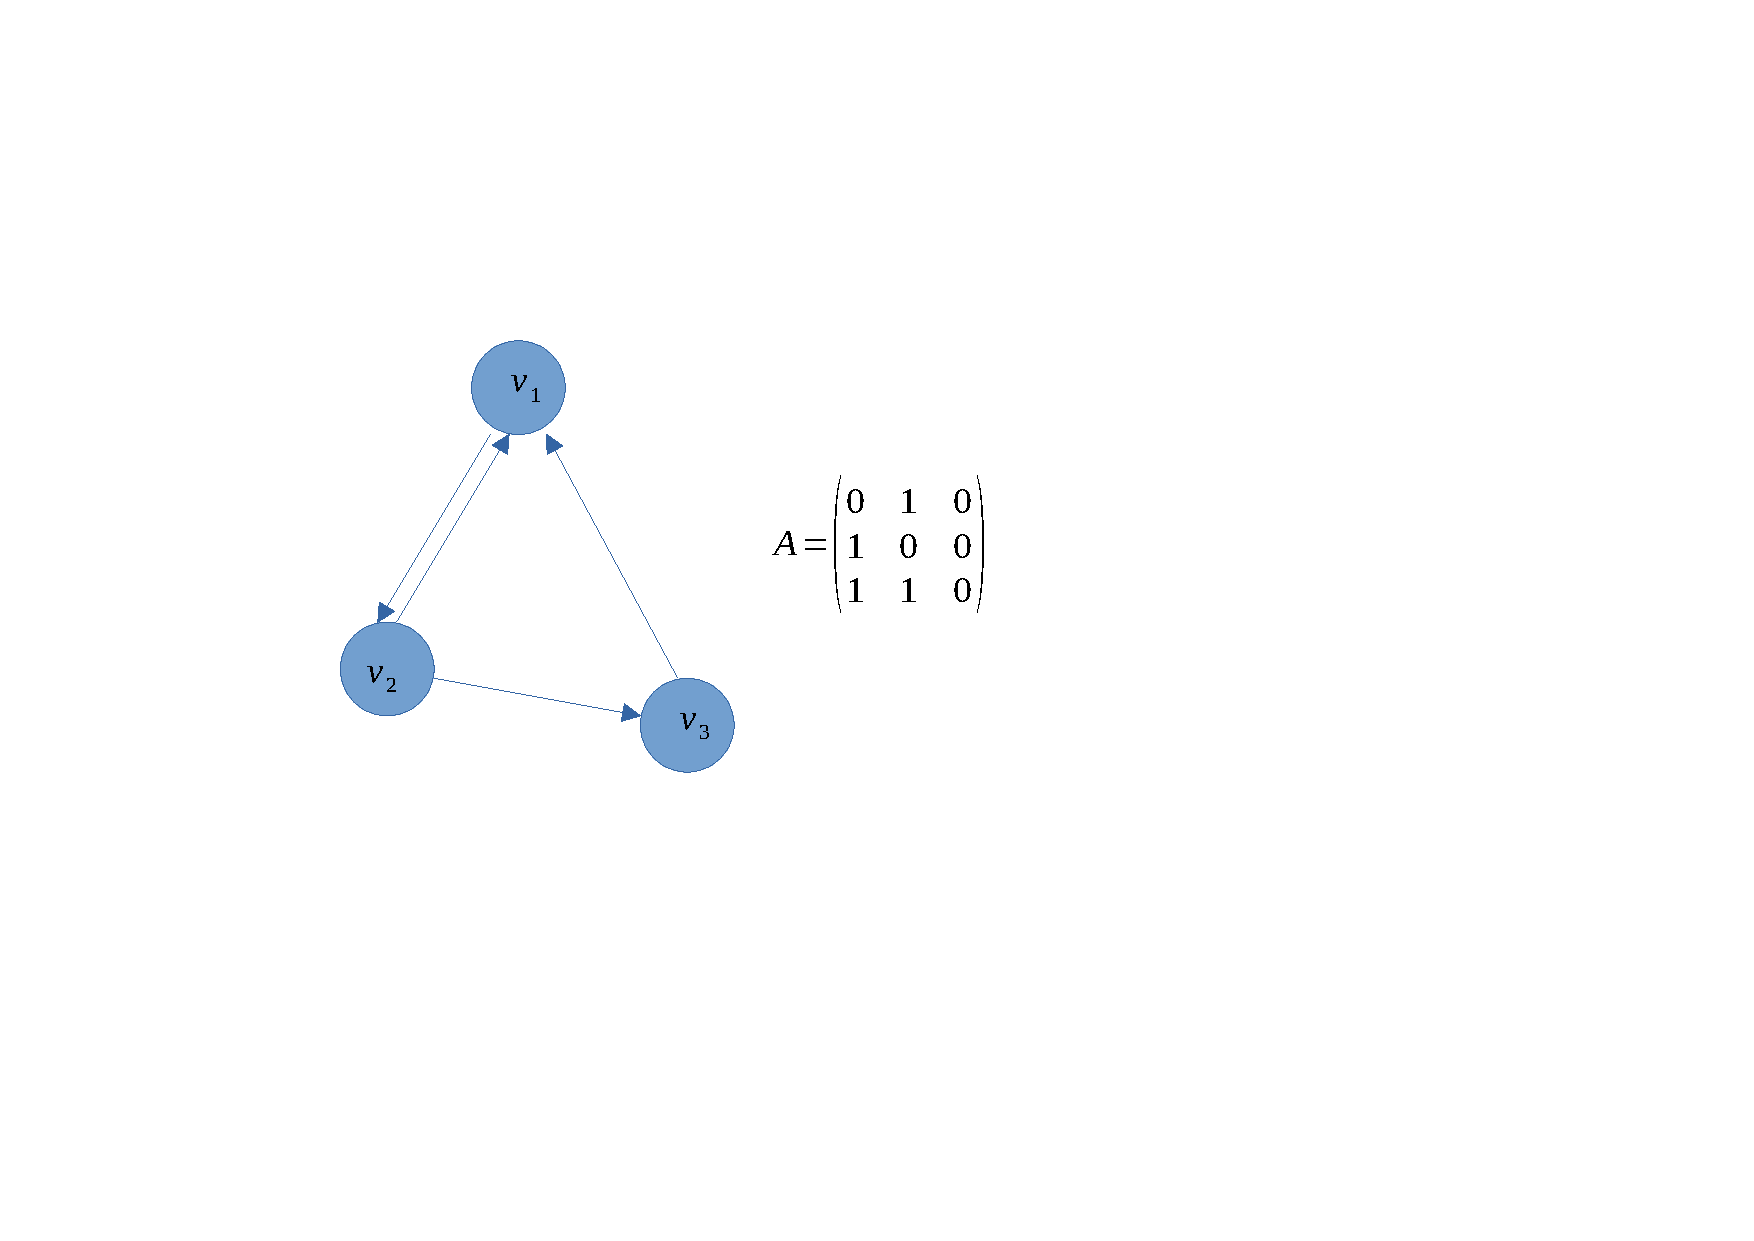
\includegraphics[width=15cm]{chapters/chapter4/graph}
	
	\caption{Graph representation}
	\label{graph}
\end{figure}
We recognize 3 main training types of GNNs and that are graph- , edge and node - oriented learning.\\
We will do only node oriented learning because we care that our data from the nodes comes dynamically right. For this we implemented two Graph Neural Layer to our work. 

\subsection{Convolutional Graph Neural Network}
First idea about graph neural network was Spectral Graph Network (SGN) \cite{sgn} in signal proccesing tasks which is based on spectrality of the modified  Laplacian in form \begin{equation}
	\mathbf{L}= \mathbf{I} - \mathbf{D}^{\frac{1}{2}}\mathbf{W}\mathbf{D}^{\frac{1}{2}} 
\end{equation}where we exchange adjecency matrix with learnable weight matrix.
Because of cost of computation and hard backpropagation, the ChebNet was introduced\cite{cheb}. 
It was dependent of fourier transformation and had high computational comlpexity.
First Kipf and Welling used both ideas and simplified Laplacian to create broadly used architecture called convolutional graph network \cite{gcn}. \\
The propagation of the layer mathematically looks like
\begin{equation}
	\mathbf{h}^{(i+1)}=\sigma(\tilde{\mathbf{D}}^{\frac{1}{2}}\tilde{\mathbf{A}}\tilde{\mathbf{D}}^{\frac{1}{2}}\mathbf{W}\mathbf{h}^{(i)})
\end{equation} where we modify adjacency matrix $\tilde{\mathbf{A}}=\mathbf{A}+ \mathbf{I}$ and $\tilde{\mathbf{D}}$ as $\tilde{\mathbf{D_{ij}}} =\sum_{j=1}^N \tilde{\mathbf{A}}_{ij}.$ 
This mathematical expression of propagation of the graph layer is equivalent to message passing on the  and aggregation on the graph from and between the neighbouring nodes. In this case with $\sum$ operator.\\ There are other types of aggregations like $\texttt{mean}$, $\texttt{sum}$ and $\texttt{sub}$. 
The default message passing and aggregation formula is defined as
\begin{equation}
\mathbf{x}_i^{(k)} = \gamma^{(k)} \left( \mathbf{x}_i^{(k-1)}, \bigoplus_{j \in \mathcal{N}(i)} \, \phi^{(k)}\left(\mathbf{x}_i^{(k-1)}, \mathbf{x}_j^{(k-1)},\mathbf{e}_{j,i}\right) \right) 
\end{equation} where $\gamma$ and $\phi$ represents MLPs and $\bigoplus$ the aggregation function. 
While the neural graph network doesn't depend on the graph structure itself, it relies on message passing and aggregation between nodes. With this understanding, we can develop more diverse designs of graph neural networks. 
%With knowledge that the neural network doesn't depend on graph structure,on the other hand it depends on massage passing and aggregation between the nodes, we can build more designs of graph neural networks.\\ 
We should not forget, that those message passing and aggregation can be parallelized and calculated on GPUs improving performance. In our use cases we will use Framework \texttt{DGL}\cite{dgl}.


\subsection{Gated Attention Network}
In paper \cite{gat} is intoduced new type of architecture which incomporates weighting factors. This weightning factors $\alpha$ shows importance of the outgoing node  to the  ingoing node in question.
The forward pass of one layer is defined as:
\begin{eqnarray}
\mathbf{z}_i^{(l)}&=&\mathbf{W}_f^{(l)}\mathbf{h}_i^{(l)}, \\
e_{ij}^{(l)}&=&\text{LeakyReLU}(\mathbf{W_a}^{(l)^T}(\mathbf{z}_i^{(l)}||\mathbf{z}_j^{(l)})),\\
\alpha_{ij}^{(l)}&=&\frac{\exp(e_{ij}^{(l)})}{\sum_{k\in \mathcal{N}(i)}^{}\exp(e_{ik}^{(l)})},\\
\mathbf{h}_i^{(l+1)}&=&\sigma\left(\sum_{j\in \mathcal{N}(i)} {\alpha^{(l)}_{ij} \mathbf{z}^{(l)}_j }\right)
\end{eqnarray}

This architecture is computationally efficient and the number of weightning factors depends on number of edges on the graph, furthermore the weightning factors are created one per edge within the multilayer perceptron. This means that the weightning factors are not bounded to the size of the graph and behaves dynamicly. % are not hard-coded and they are calculated in dependence with a graph structure.
For better training and preventing overfitting, we can set a dropout at MLP which creates weightning factors\cite{att}, it is even suggested for  the small graphs.












\section{Graph Hamiltonian Neural Network}
This architecture is inspired on implementation of HNN\cite{hnn} and paper \cite{GNNODE}. In the paper they implemented own Graph Neural Network with complicated architecture called GN, which has many applications in Deep Leraning.  They tried to implement HOGN model.
In our case we will use conventional GNN model to create the same.
In our cases our graph will built without loop nodes. Nodes with edge connected to the starting node. With many trials we achieve same valued features at the nodes using \texttt{sum} or \texttt{mean} aggregation at fully connected graph, With discarding self loops we don't have this problem anymore.\\  It is important that the output of our Graph network is a scalar value because it represents $\mathcal{H}$. Without this condition, auto differentiation won't work. 
There is the forumla for GHNN.
\begin{eqnarray}
	H_{\Theta} &=& \mathbf{f}(\mathbf{x}|\boldsymbol{\Theta})=\text{GNN layer }(\mathbf{x})\\
	\frac{d\mathbf{x}}{dt} &=& \left[\frac{\partial H_{\Theta}}{\partial\mathbf{p}}(\mathbf{x}),-\frac{\partial H_{\Theta}}{\partial\mathbf{q}}(\mathbf{x})\right]^T
\end{eqnarray}
The Graph Neural Network can be made with more layers and we can add activation functions. In the experiments we used GAT layer.\\
This model gives trajectory trough using of one ode solvers. Its architecture you can observe in Figure \ref{ghnn}.
\begin{figure}[h!]
	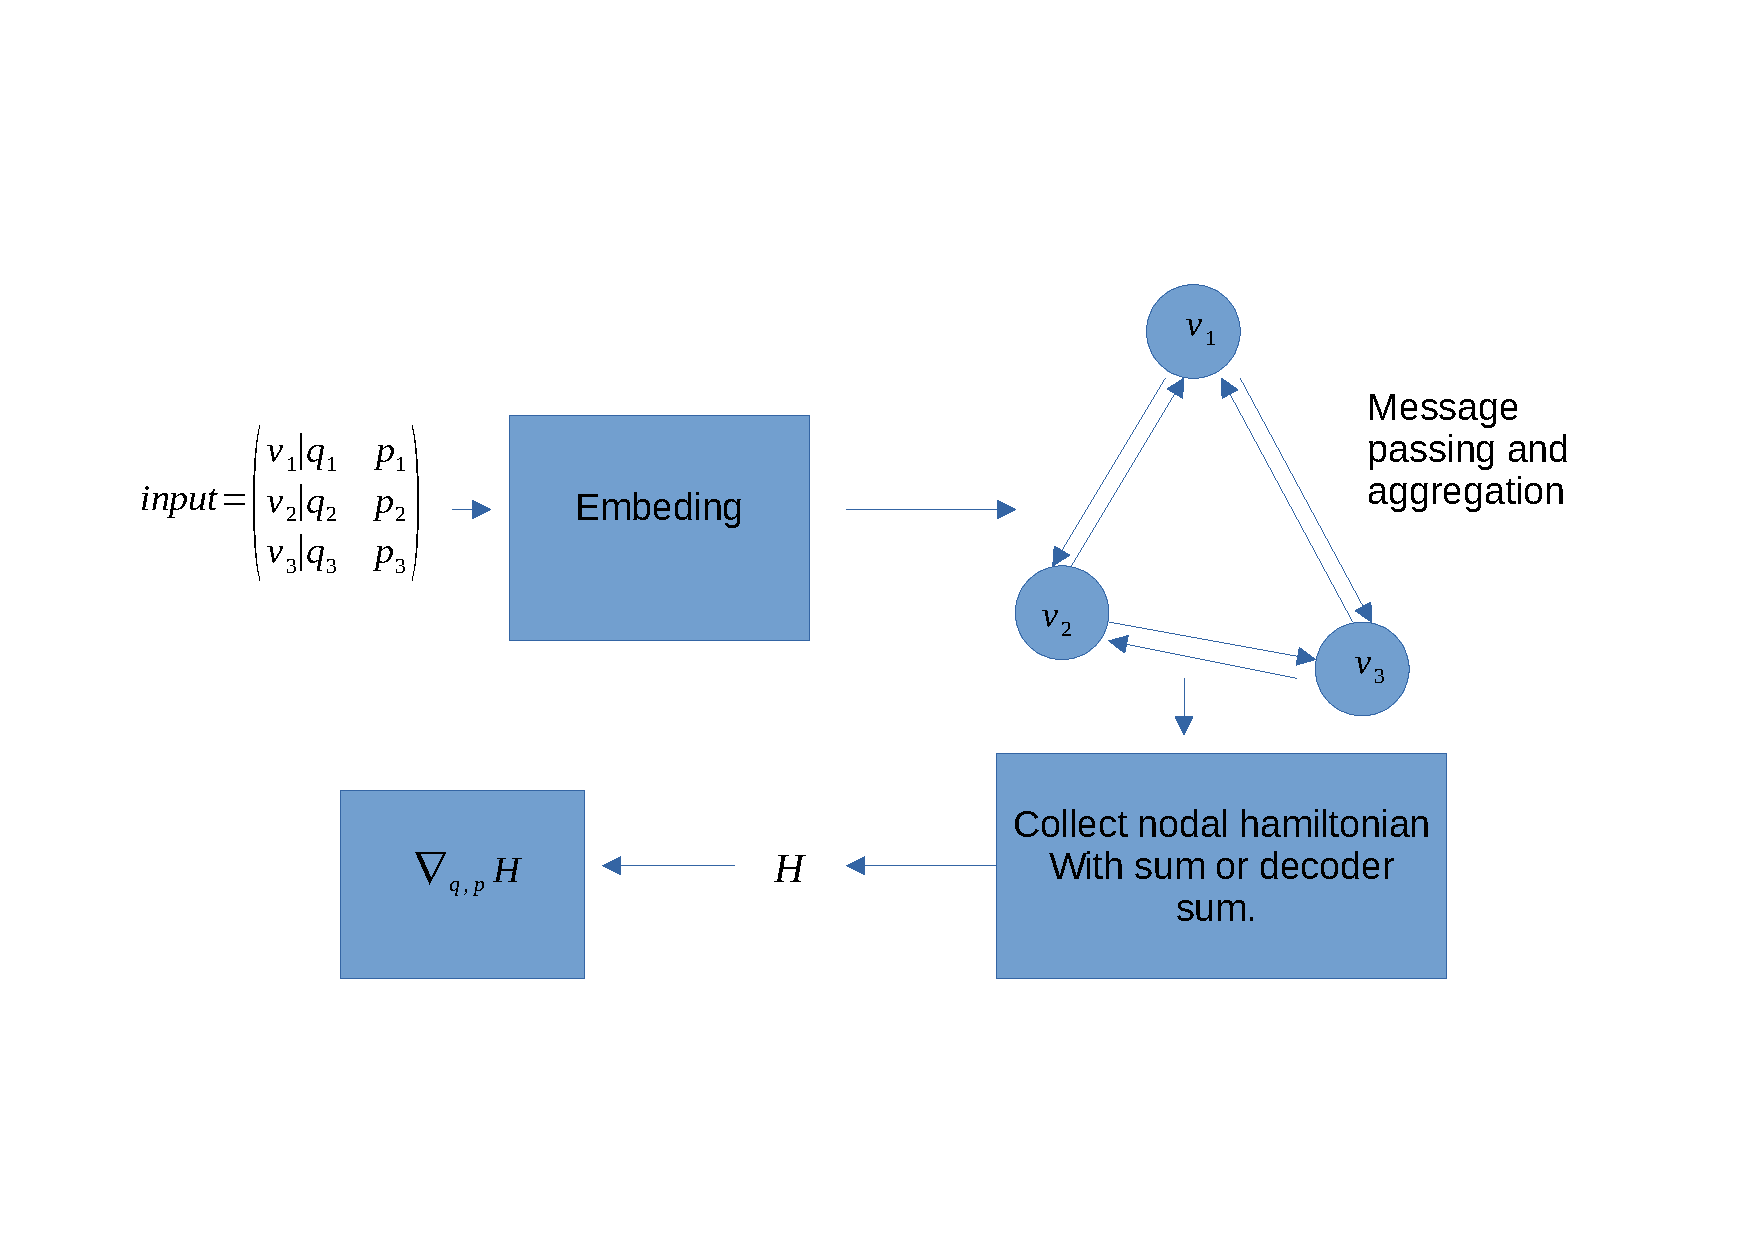
\includegraphics[width=15cm]{chapters/chapter4/ghnn}
	\caption{Architecture of Graph Neural Hamiltonian Network}
	\label{ghnn}
\end{figure}
\section{Improved Graph Hamiltonian Neural Network}
As GHNN mentioned before did't show very good performance we were forced to find some new architecture. We found new layer which we could use and it is inspired by paper \cite{wave}. The adapting adjecency matrix is very interesting concept but in the scope of coding, the \texttt{DGL} don't allow fitting the adjecency matrix.\\
In the paper adaptive adjecency was calculated as
\begin{equation}
	\mathbf{A_{adp}} = Softmax(ReLU(\mathbf{E_1}\mathbf{E_2^T})),
\end{equation}
This procedure looks very alike attentional coefficient calculation.
We made our architecture for one layer as

\begin{eqnarray}
	\mathbf{y}_{gcn} &=& GCN(\mathbf{x}),\\
	\mathbf{y}_{gat} &=& GAT(\mathbf{x}),\\
	\mathbf{y}_{mlp} &=& MLP(\mathbf{y}_{gcn}|\mathbf{y}_{gat}),\\
	\mathbf{y} &=& \mathbf{y}_{gcn}+\mathbf{y}_{gat}+\mathbf{y}_{mlp}\\
	H_{\Theta} &=& \sum \mathbf{y} \text{   sum of the all features}\\
	\frac{d\mathbf{x}}{dt} &=& \left[\frac{\partial H_{\Theta}}{\partial\mathbf{p}}(\mathbf{x}),-\frac{\partial H_{\Theta}}{\partial\mathbf{q}}(\mathbf{x})\right]^T
\end{eqnarray}
We used the multilayer perceptron as some sort of decoder which uses concatenated input of outputs from GAT and GCN layer. We summed everything together.\\
We will use it in some of our experiments. The architecture can be observed in Figure \ref{improvedGHNN}

\begin{figure}[h!]
	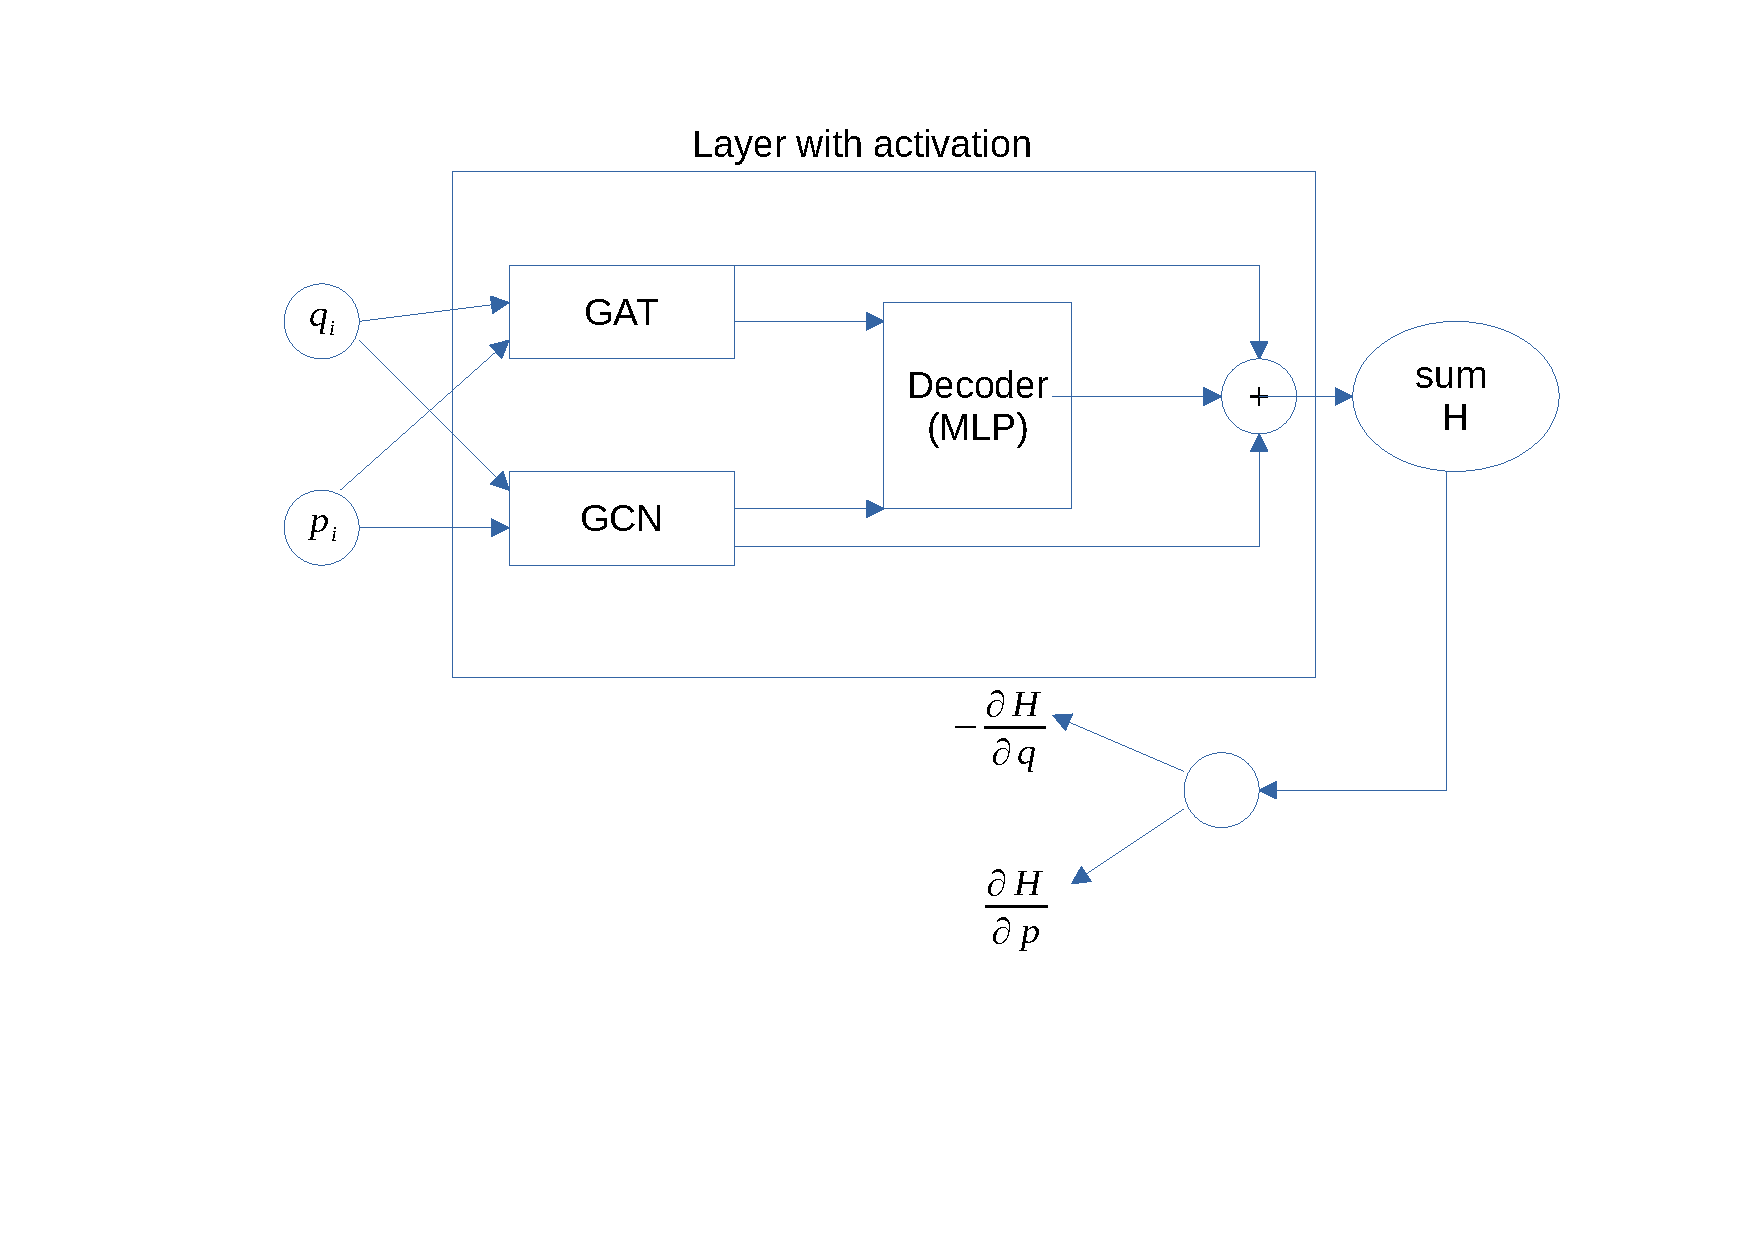
\includegraphics[width=15cm]{chapters/chapter4/improved_GHNN.pdf}
	
	\caption{Architecture of improved GHNN}
	\label{improvedGHNN}
\end{figure}

 

 



\section{Gated Recurrent Graph Hamiltonian Neural Network - GRUGHNN}
In previous section we introduced the GHNN, which is base an Hamiltonian layer and ode-solver. This architecture is not different but improved with a GRU unit at the beginning of the input. this model is equivalent to the GRU stepper but we added a GHNN in it. It is Graph Neural Network with a memory feature. If we compare this model to spatio-temporal models you can see similarities. Only two models have similar architecture to this. We will mention Gated Graph Sequence Neural Network\cite{GGSNN} and GNN-GRU\cite{gnngru}, but they don't use auto differentiation. Without autodifferentiation we can not call our architectures as "hamiltonian". 

\begin{eqnarray}
	[\mathbf{a}_i, \mathbf{h}_{i+1}] &=&  \text{GRU}(\mathbf{x}_i,\mathbf{h}_i)\\
	 H_i&=& \text{GNN}(\mathbf{a}_i)\\
	 \mathbf{v}_i&=&\left[\frac{\partial H_{i}}{\partial\mathbf{p}}(\mathbf{x}),-\frac{\partial H_{i}}{\partial\mathbf{q}}(\mathbf{x})\right]^T\\
	 \mathbf{x}_{i+1} &=& \mathbf{x}_i + \mathbf{v}_i \cdot dt
\end{eqnarray}
Its architecture you can observe in Figure \ref{GRUGHNN}
\begin{figure}[h!]
	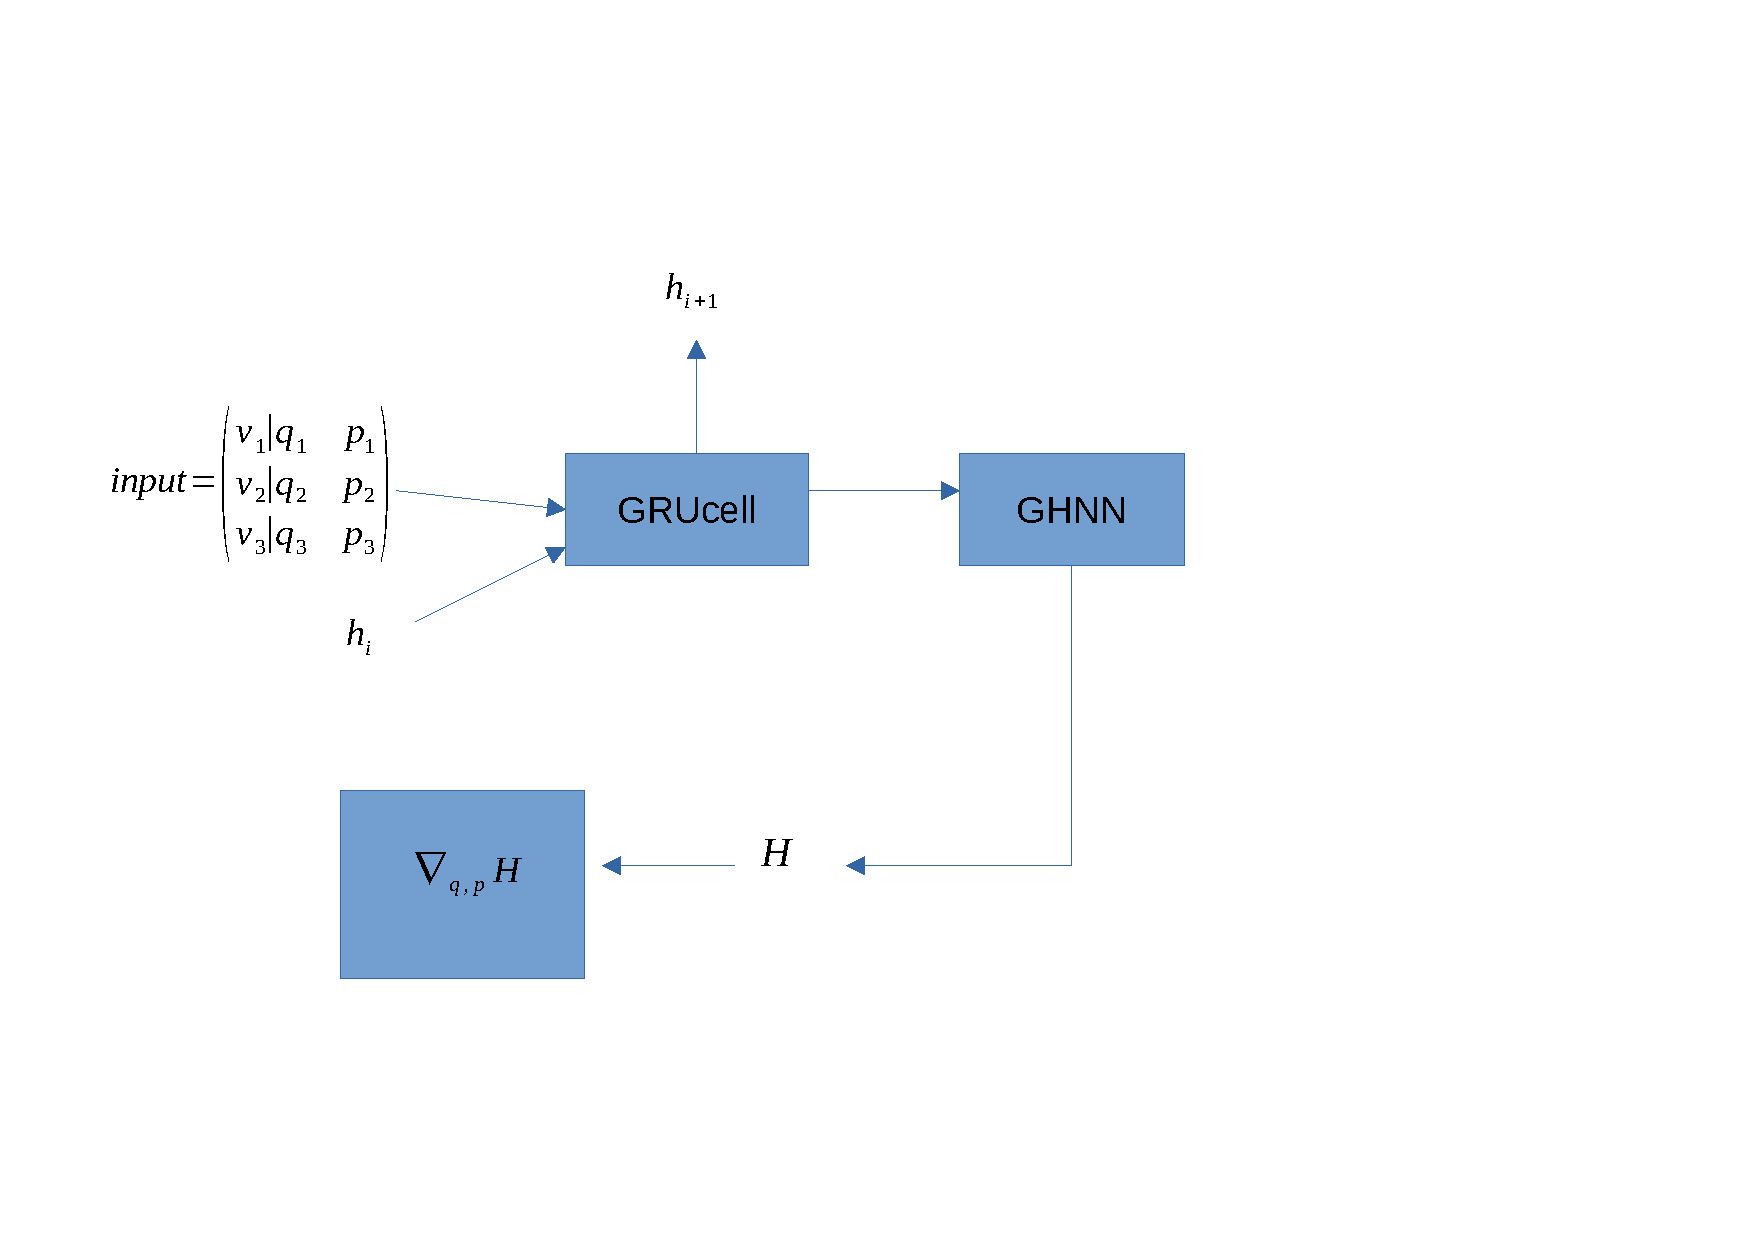
\includegraphics[width=15cm]{chapters/chapter4/GRUGHNN}
	
	\caption{Architecture of GRUGHNN}
	\label{GRUGHNN}
\end{figure}
\section{Training for Physics Informed Models}
As we introduced the models we can observe that they are intended to be used in some ODE solver. That means that the data and our datasets are time series oriented. The specifics of time-series data are they have three dimensions which are time $t$, sample space $s$ and feature space $f$. Let us define it as $\mathcal{V}^{t,s,f}$.\\
This sample is very specific, and in case of mini-batching we can't just pick some values and make a batch , the data follow the timeflow which means, that we need to create a batches specify the length of the sequence and how many sequences are in the sample. We call it \texttt{timebatch size} and \texttt{batch size}.\\
Such \texttt{time batches} we call snapshots $\mathcal{V}^{t,f}$, because it represents recorded confined sequence for one specific inital value. For example we have a sequence with 128 timepoints and with $\texttt{timebatch size} = 32$ we can make 96 snapshots with sequence size 32. Even if the data repeats itself it is important that we need to use many initial values as possible.\\
If we have to many samples or to big sequence we can implement \texttt{stride} technique. We specify which sequence will we recorded for our dataset. For example with \texttt{stride}=4 we specify that we want every forth inital value and its sequence recorded. Resulting in smaller dataset.\\
In case of graph batched data we need to be careful. First our sample space will change in $\mathcal{V}^{s \times n,t,f}$ where  $n$ means nodes. First we need to transform our made snapshots to graph structure, which means to place the features at their corresponding nodes and we get $\mathcal{V}^{n,t,f}$. The batching is very straight forward, it could be called "stacking the graphs". We make one big graph using $s$ times graphed independent snapshots. We call it independent because there are no edge connections between other graphs and propagating between nodes of the graphs is done in parallel.\\
In case of Hamiltonian Neural Networks and extracting a hamiltonian values of the independent graphs we suggest to unbatch it first and create a normal batch of hamiltonian values. It makes calculation of hamiltonian easier. If you calculate from the batched form, you need to be careful because the  hamiltonian can be incorrect because, we need to sum the features in every  independent graph separately.      



\chapter{Experiments}
Now we perform comparison experiments to compare the state of the art models, common models and PINN(Graph Neural Network) models. Our goal is implicitly train our dataset to proposed networks in fully supervised manner. In cases of PINN models we supervise trajectory, vectorfield and hamiltonian energy made by the model itself. 

\section{Experimentation of the Models on the Datasets}
In this section we experiment on following models
\begin{itemize}
	\item Multilayer perceptron
	\begin{itemize}
		\item 4 layers with size: oscilator 128,twobody 256, threebody 512
		\item activations: tanh, relu, relu, identity
	\end{itemize}
	
	\item NeuralODE
	\begin{itemize}
		\item 3 layers with size oscilator 128, twobody 256, threebody 512
		\item activations: tanh, relu, identity
	\end{itemize}
	
	\item GRU - size: oscilator 256,
	\item RNN - size: oscilator 256,
	\item GRU time stepper - size: oscilator 256, twobody 256, threebody 512
	\item RNN time stepper - size: oscilator 256, twobody 256, threebody 512
\end{itemize}
on various datasets made with hamiltonan equation.
We used optimizer AdamW and loss function
\begin{equation}
	Loss = \text{Huber}(\mathbf{y},\hat{\mathbf{y}})
\end{equation}
For the Hamiltonian accuracy we used MSE Loss. We need to disclaim that the hamiltonian is not part of the model. It predefined function by the real model, we just use it to see if the trajectory prediction shows possible conservation of energy inside the model as a black box problem. 
\subsection{Harmonic Oscillator}
In previous chapter we disscused about creation of the Oscilator Dataset.
In this Experiment we chose $k=0.8$ and $m=1.0$ and made 30 trajectories for training data and 3 trajectories for test data with 128 time points in one period.\\
The trajectories are different because we set our Hamiltonian/Total Energy in region $H=[5,15]$.\\ We predict very well generalization because we are working with following type of equation\begin{equation}
	\dot{\mathbf{x}} = \mathbf{A}\mathbf{x}.
\end{equation} The matrix $\mathbf{A}$ for every trajectory is fully constant and it should be trivial case.\\
We train the models with "rollout" technique. It is training step where we take beginning of our relevant trajectory and we let the model to predict rest of trajectory.\\ 
We managed to make batch-wised training making the snapshots of the trajectory with length of 32 time points. We took 30 train trajectories and 3 test trajectories.  \\
With such training we got following results in figures \ref{osci_loss},\ref{osci_traj}: 
\begin{itemize}
	\item Multilayer perceptron\\
	After observation we can conclude that the baseline as MLP did learned hamiltonian system but not accurate enough. In this case which is learned for 1000 epochs we see that we have maybe overtrained the network. From the energy accuracy we can see that the metric for energy accuracy which is made over the trajectory is little bit to high in all of the epochs. 


	\item NeuralODE\\
	In this case we trained properly the hamiltonian system. Energy dosen't show conservative property but the difference between true hamiltonian isn't to high. In comparison with MLP case the energy accuracy here is more accurate then MLP in every epoch. 

	\item GRU\\
	In this case we see classic example of overtraining, After 500 epoch the losses and energy accuracy started to rise and a evaluation sample shows similar result to MLP case.

	\item RNN
	In this case RNN shows overall good performance and it could be compare to NeuralODE case. The trajectory dosen't show periodic movement, but overall the hamiltonian shows conservative property

	\item GRU Time Stepper\\
	GRU stepper is very interesting hamiltonian accuracy shows better perfomance the NeuralODE. in our Evaluation sample we got result where movement isn't periodic and overshots the end point. The Hamiltonian of evaluation sample rises. We have assumption that we see here numerical approximation error due to model architecture.  


	\item RNN Time Stepper\\
	This model shows interesting behaviour in which evaluation plot looks similar to GRU Stepper but the energy hold conservative proiperty.
	The enrgy accuracy is in the rang with NeuralODE.

\end{itemize}

\begin{figure}[H]
	
	\centering
	\begin{subfigure}[b]{0.3\textwidth}
		\centering
		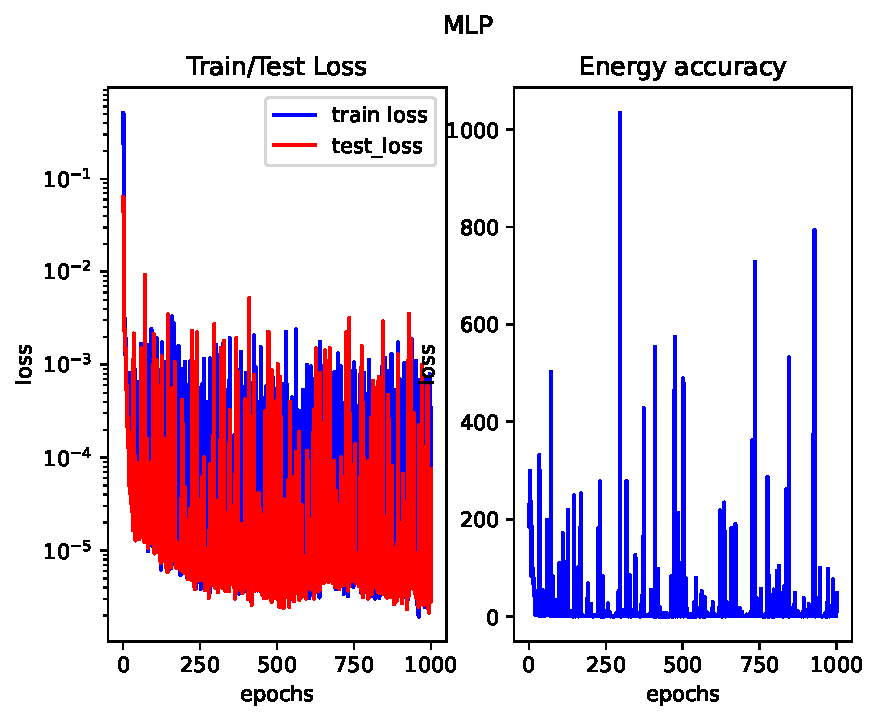
\includegraphics[width=\textwidth]{chapters/chapter5/osci_mlp_loss.pdf}
		\caption{MLP}
	\end{subfigure}
	\hfill
	\begin{subfigure}[b]{0.3\textwidth}
		\centering
		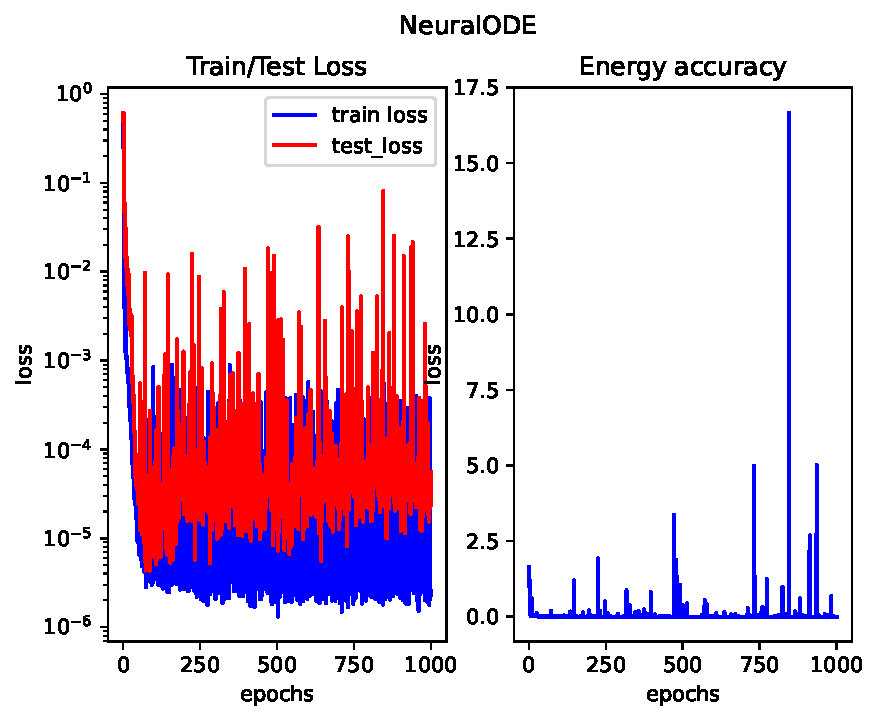
\includegraphics[width=\textwidth]{chapters/chapter5/osci_ode_loss.pdf}
		\caption{ODE}
	\end{subfigure}
	\hfill
	\begin{subfigure}[b]{0.3\textwidth}
		\centering
		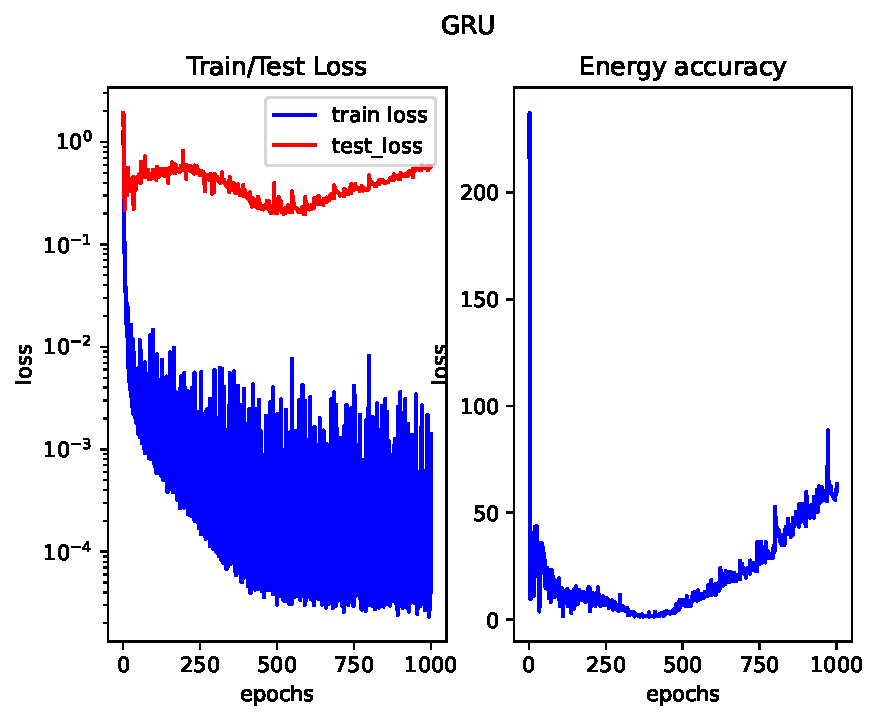
\includegraphics[width=\textwidth]{chapters/chapter5/osci_gru_loss.pdf}
		\caption{GRU}
	\end{subfigure}
	
	\vspace{0.5cm} % Adds vertical space between rows
	
	\begin{subfigure}[b]{0.3\textwidth}
		\centering
		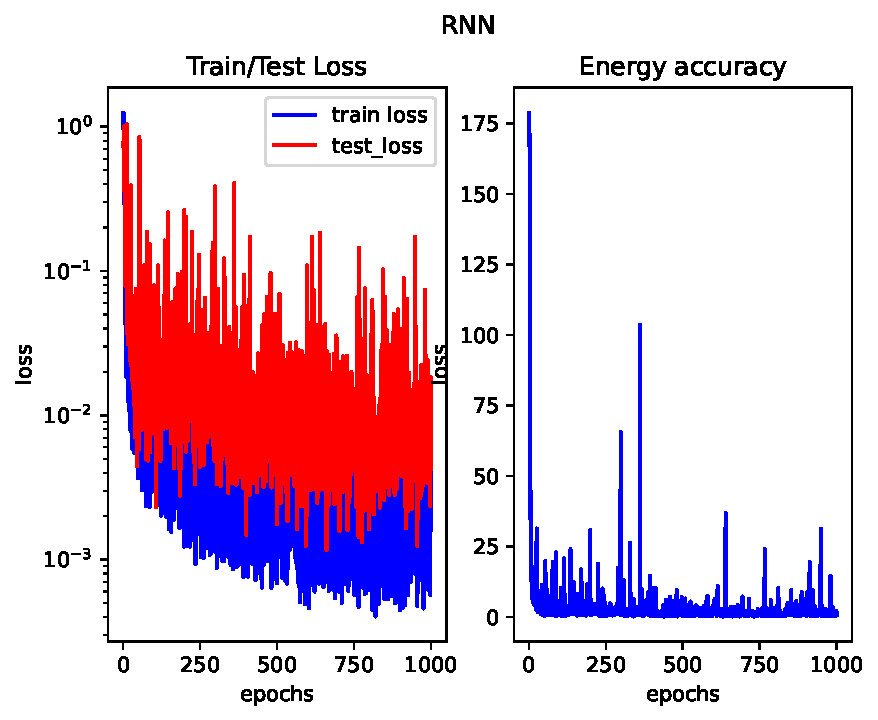
\includegraphics[width=\textwidth]{chapters/chapter5/osci_rnn_loss.pdf}
		\caption{RNN}
	\end{subfigure}
	\hfill
	\begin{subfigure}[b]{0.3\textwidth}
		\centering
		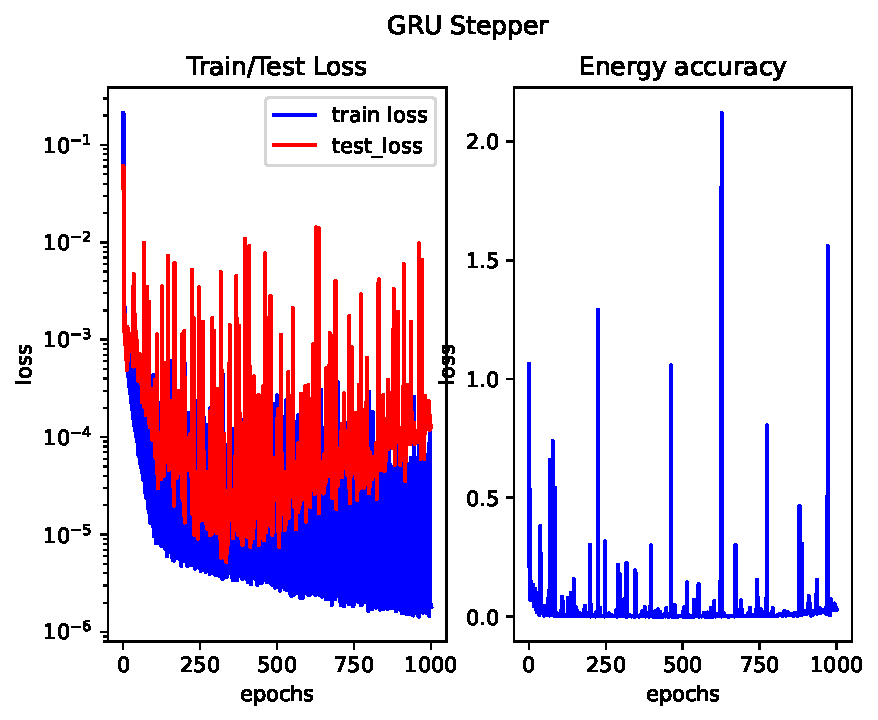
\includegraphics[width=\textwidth]{chapters/chapter5/osci_gre_loss.pdf}
		\caption{GRU Stepper}
	\end{subfigure}
	\hfill
	\begin{subfigure}[b]{0.3\textwidth}
		\centering
		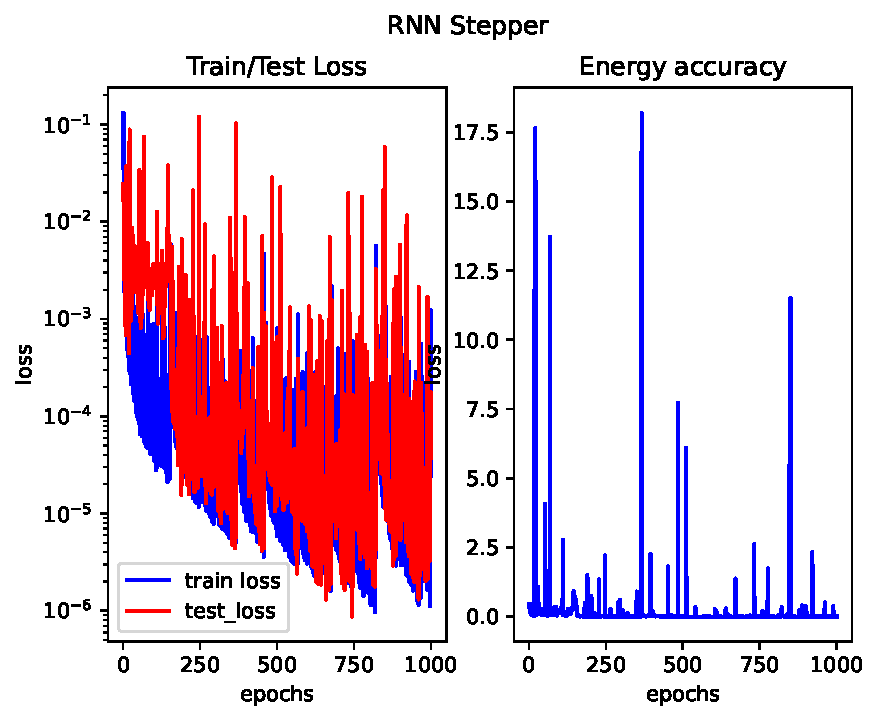
\includegraphics[width=\textwidth]{chapters/chapter5/osci_rne_loss.pdf}
		\caption{RNN stepper}
	\end{subfigure}
	
	\caption{Losses and energy accuracy on various neural models(Oscilator)}
	\label{osci_loss}
\end{figure}

\begin{figure}[H]

	\centering
	\begin{subfigure}[b]{0.3\textwidth}
		\centering
		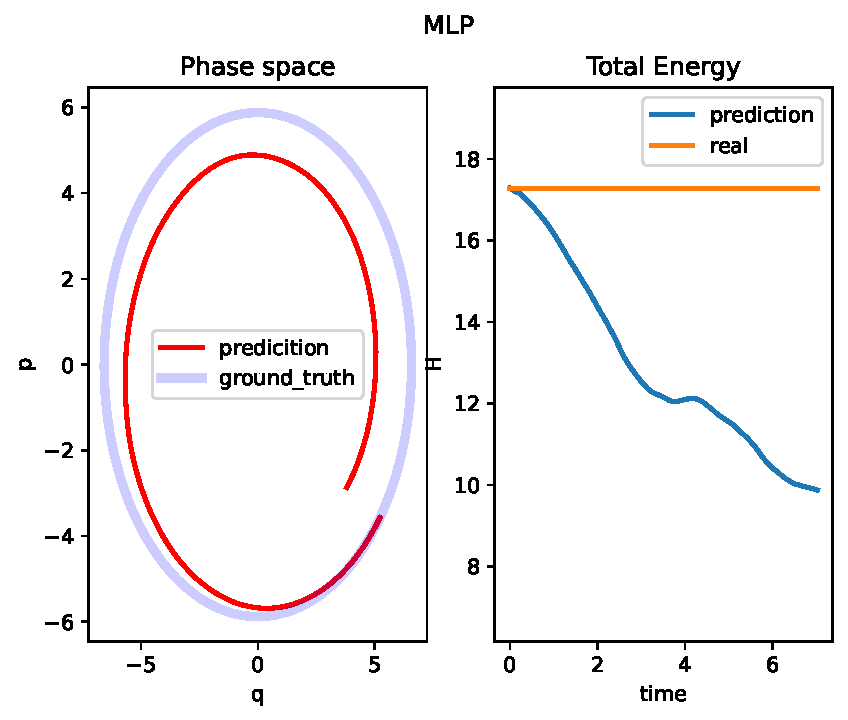
\includegraphics[width=\textwidth]{chapters/chapter5/osci_mlp_ps.pdf}
		\caption{MLP}
	\end{subfigure}
	\hfill
	\begin{subfigure}[b]{0.3\textwidth}
		\centering
		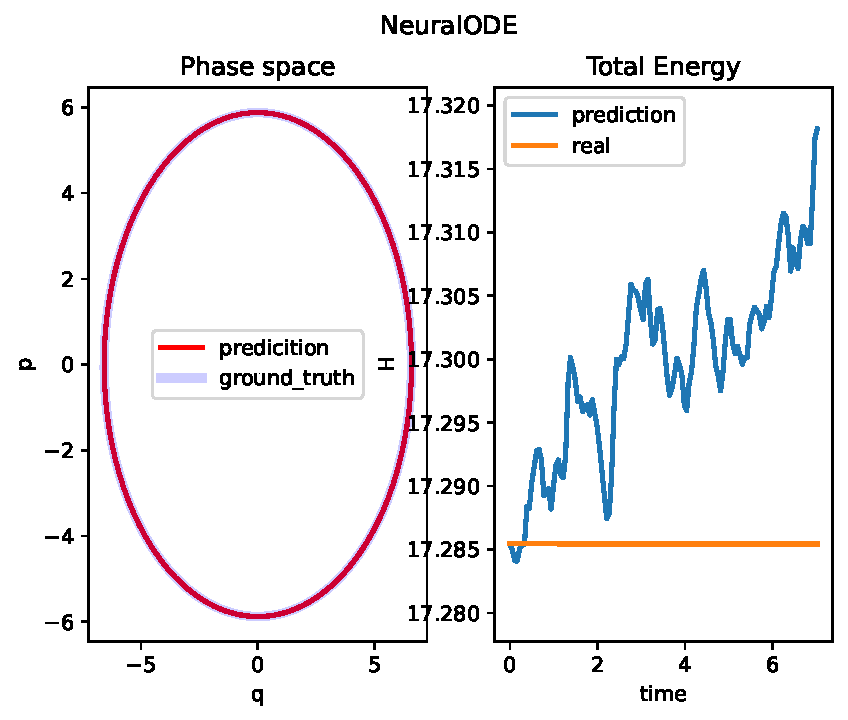
\includegraphics[width=\textwidth]{chapters/chapter5/osci_ode_ps.pdf}
		\caption{ODE}
	\end{subfigure}
	\hfill
	\begin{subfigure}[b]{0.3\textwidth}
		\centering
		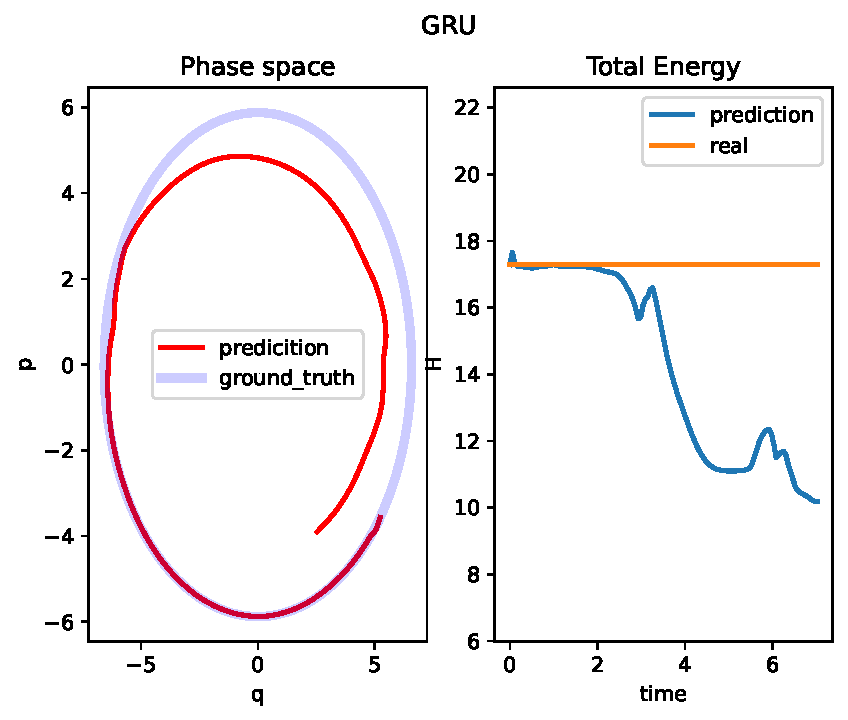
\includegraphics[width=\textwidth]{chapters/chapter5/osci_gru_ps.pdf}
		\caption{GRU}
	\end{subfigure}
	
	\vspace{0.5cm} % Adds vertical space between rows
	
	\begin{subfigure}[b]{0.3\textwidth}
		\centering
		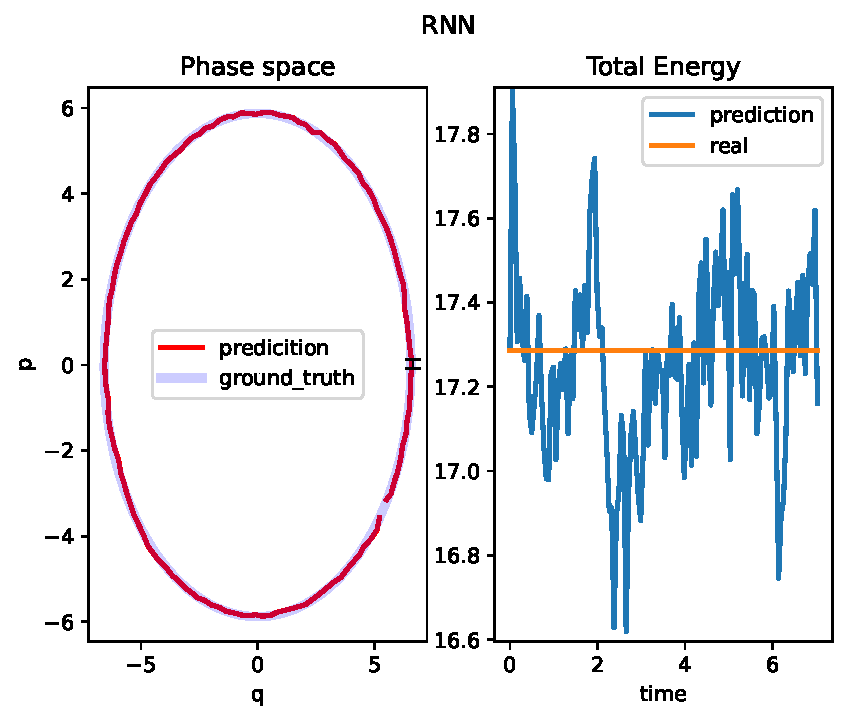
\includegraphics[width=\textwidth]{chapters/chapter5/osci_rnn_ps.pdf}
		\caption{RNN}
	\end{subfigure}
	\hfill
	\begin{subfigure}[b]{0.3\textwidth}
		\centering
		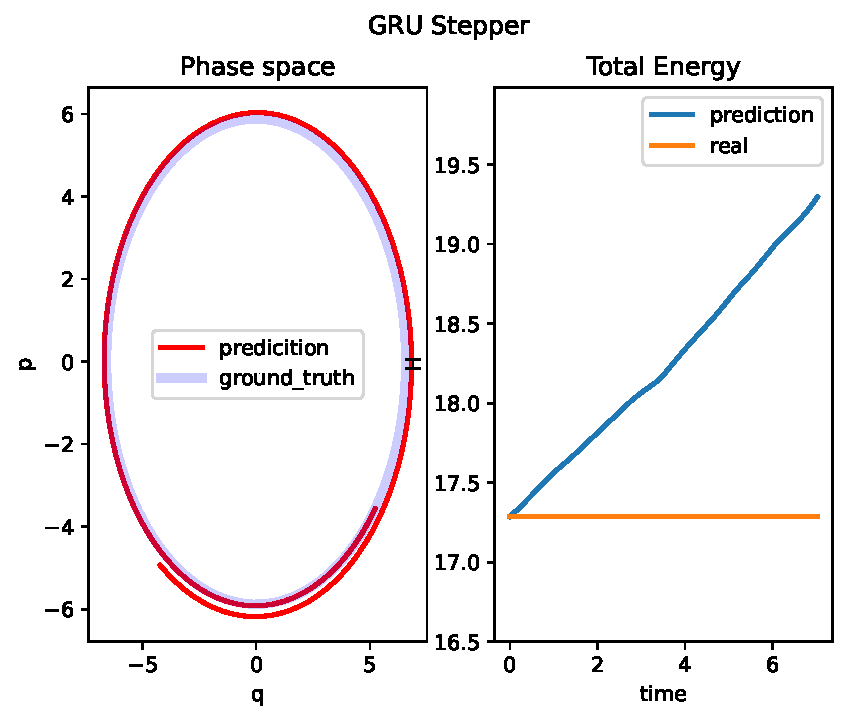
\includegraphics[width=\textwidth]{chapters/chapter5/osci_gre_ps.pdf}
		\caption{GRU Stepper}
	\end{subfigure}
	\hfill
	\begin{subfigure}[b]{0.3\textwidth}
		\centering
		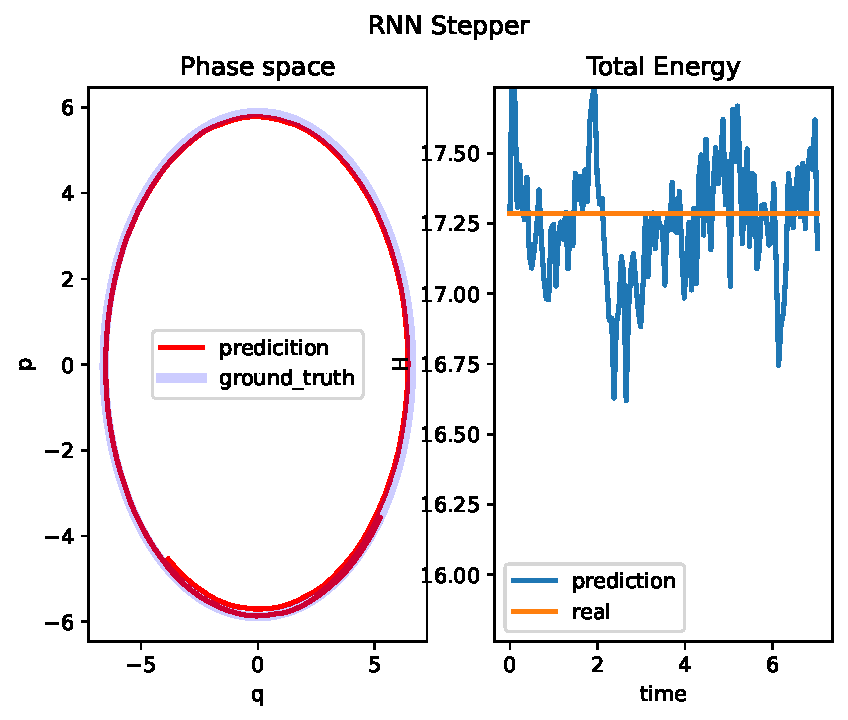
\includegraphics[width=\textwidth]{chapters/chapter5/osci_rne_ps.pdf}
		\caption{RNN stepper}
	\end{subfigure}
	
	\caption{Evaluation of the sample on the models, Trajectory and Energy(Oscilator)}
	\label{osci_traj}
\end{figure}
	

 

\subsection{Twobody-problem}
In previous chapter we disscused about creation of the Twobody Dataset.
In this Experiment we chose masses $m=\{1.0,3.0\}$ and $G=1$, we made 30 trajectories for training data and 3 trajectories for test data with 128 time points in one period.\\
The train data is batched an we have done batched leraning\begin{equation}
	\dot{\mathbf{x}} = \mathbf{A}(||\mathbf{q_1(t=0)}||)\mathbf{x},\text{  }\mathbf{x} = \begin{bmatrix}
		\mathbf{q}\\
		\mathbf{p}
	\end{bmatrix}
\end{equation} The matrix $\mathbf{A}$ is constant only for dynamics of one trajectory.\\
We train the models with "rollout" technique, exactly like explained in the oscilator case and we got following results \ref{body2_loss}, \ref{body2_traj}, \ref{body2_ps}.
\begin{itemize}
	\item Multilayer perceptron\\
	From the loss figure we see that the model has learned a hamiltonian system. Even the energy accuracy looks very stable. On the other hand the evaluation plot is little bit inaccurate.
	
	
	\item NeuralODE\\
	The trajectory is accurate and energy at evaluation sample looks that hold conservative property. Over all it is most accurate model of all.
	
	
	\item GRU\\
	similar to MLP the trajectory is little bit inaccurate but the energy shows conservative property.
	
	\item RNN\\
	It looks similar to GRU but the trajectory looks like it osclates around ground truth data 

	\item GRU Time Stepper\\
	The trajectory and energy on the evaluation sample looks inaccurate but it follows the flow of trajectory. ´

	\item RNN Time Stepper\\
	It has same characteristics as GRU Stepper but it has slightly worse perforamnce,
	
\end{itemize}

\begin{figure}[H]
	\centering
	\begin{subfigure}[b]{0.3\textwidth}
		\centering
		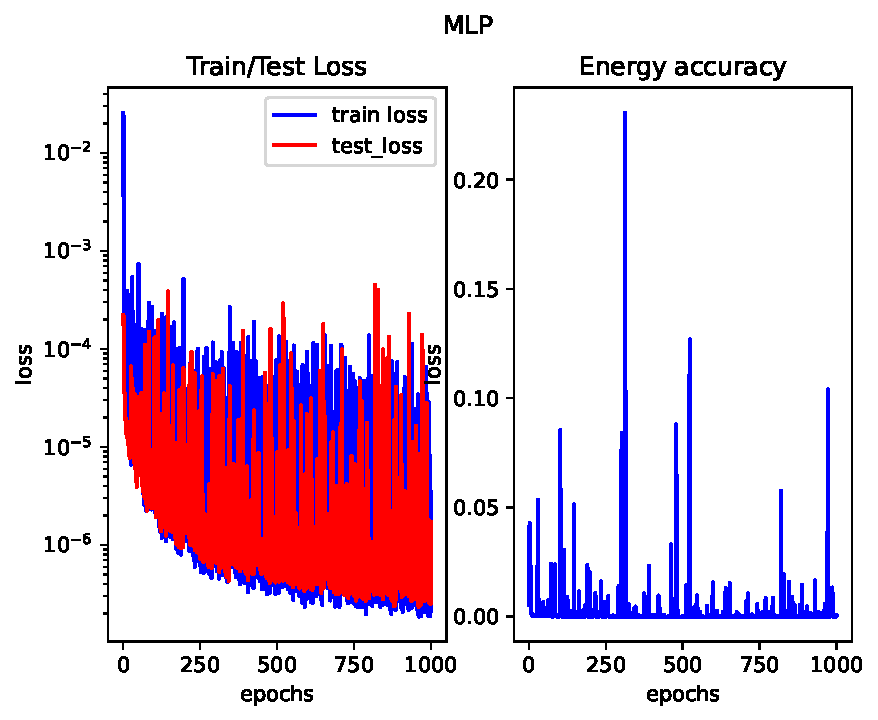
\includegraphics[width=\textwidth]{chapters/chapter5/body2_mlp_loss.pdf}
		\caption{MLP}
	\end{subfigure}
	\hfill
	\begin{subfigure}[b]{0.3\textwidth}
		\centering
		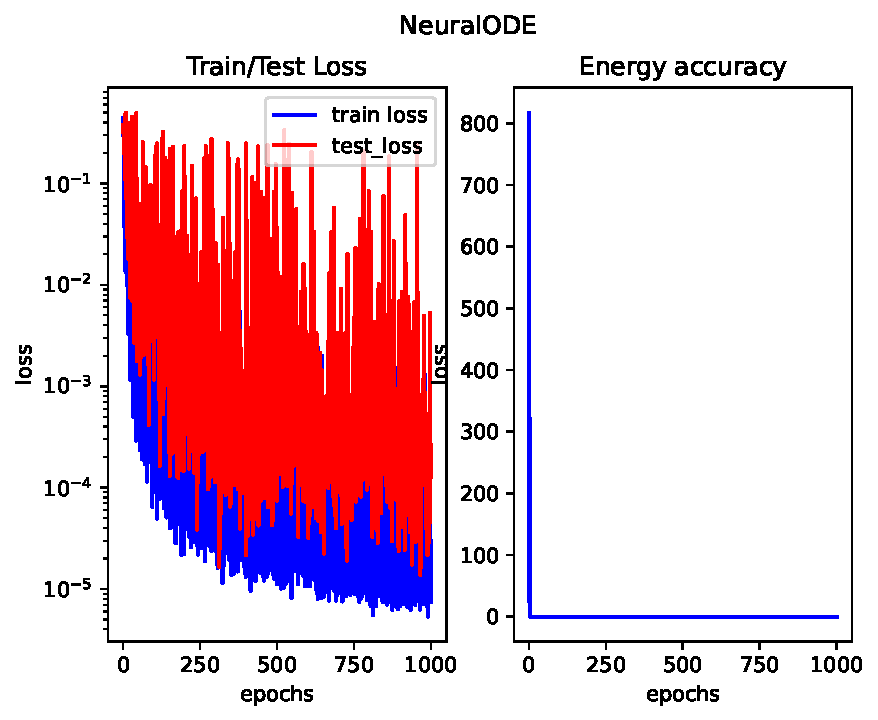
\includegraphics[width=\textwidth]{chapters/chapter5/body2_ode_loss.pdf}
		\caption{ODE}
	\end{subfigure}
	\hfill
	\begin{subfigure}[b]{0.3\textwidth}
		\centering
		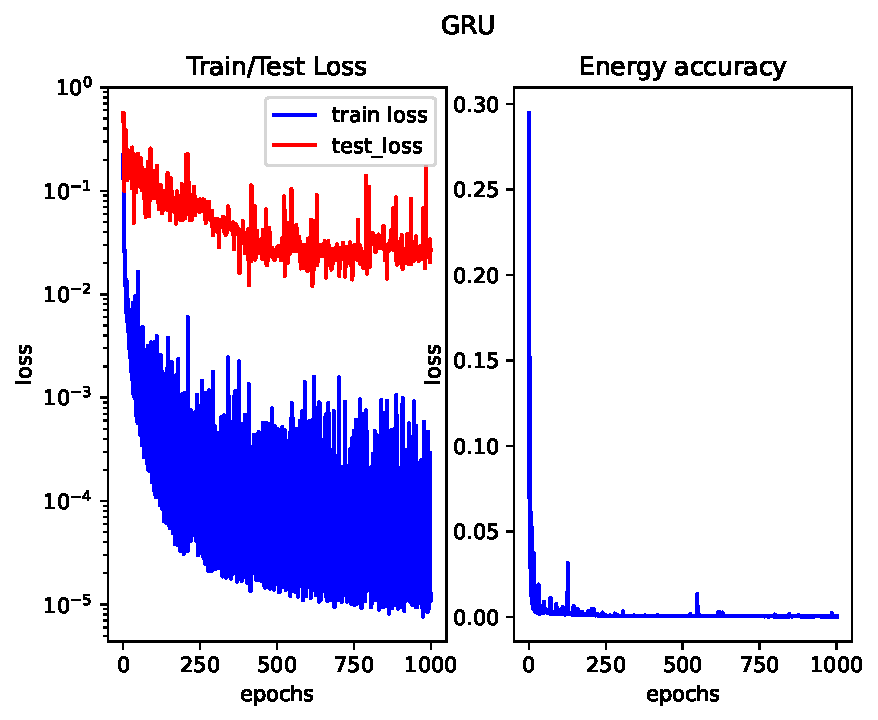
\includegraphics[width=\textwidth]{chapters/chapter5/body2_gru_loss.pdf}
		\caption{GRU}
	\end{subfigure}
	
	\vspace{0.5cm} % Adds vertical space between rows
	
	\begin{subfigure}[b]{0.3\textwidth}
		\centering
		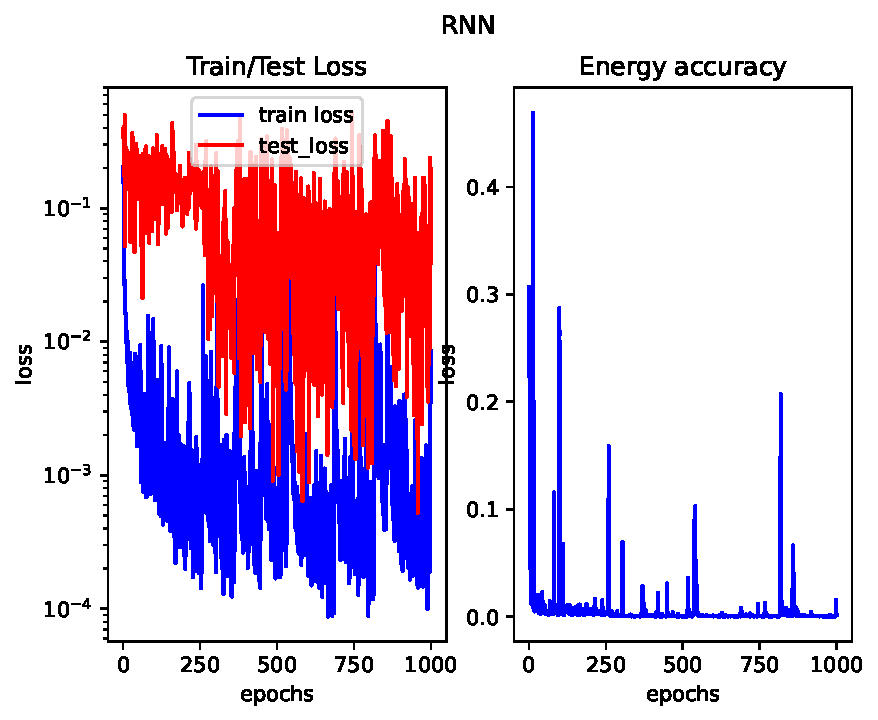
\includegraphics[width=\textwidth]{chapters/chapter5/body2_rnn_loss.pdf}
		\caption{RNN}
	\end{subfigure}
	\hfill
	\begin{subfigure}[b]{0.3\textwidth}
		\centering
		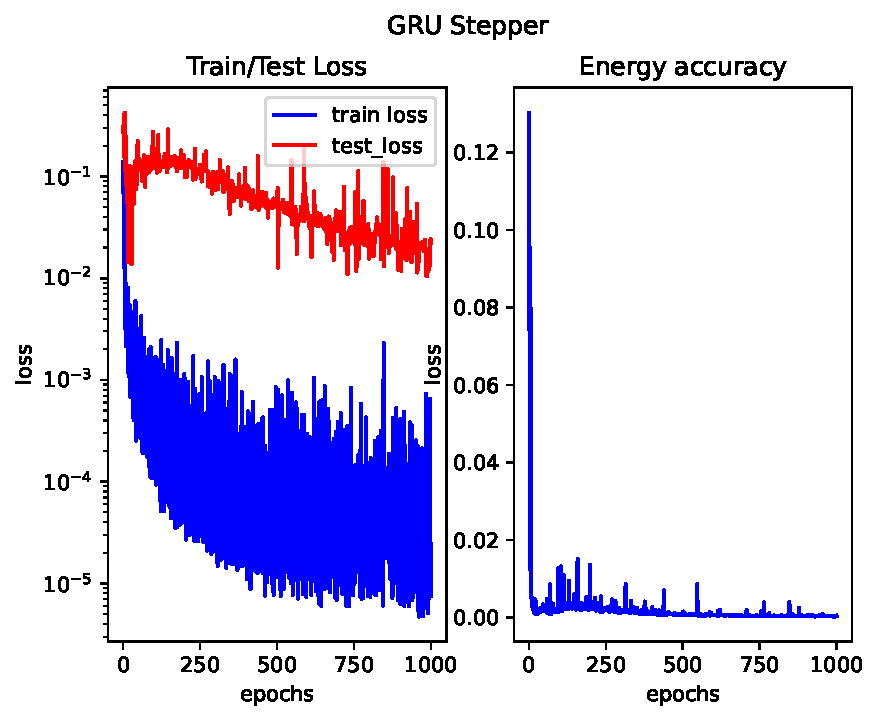
\includegraphics[width=\textwidth]{chapters/chapter5/body2_gre_loss.pdf}
		\caption{GRU Stepper}
	\end{subfigure}
	\hfill
	\begin{subfigure}[b]{0.3\textwidth}
		\centering
		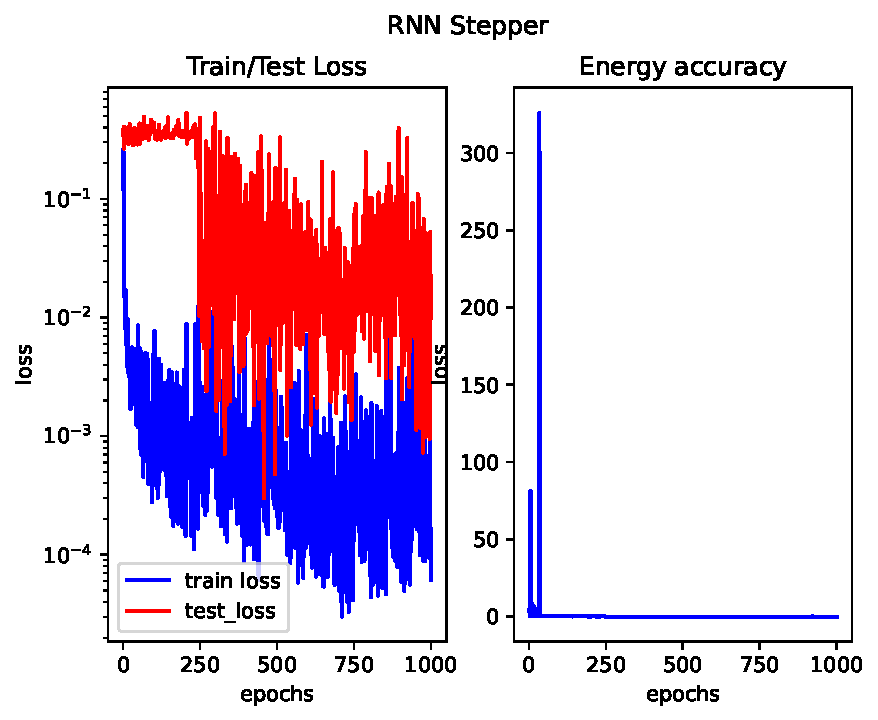
\includegraphics[width=\textwidth]{chapters/chapter5/body2_rne_loss.pdf}
		\caption{RNN stepper}
	\end{subfigure}
	
	\caption{Losses and energy accuracy on various neural models(Oscilator)}
	\label{body2_loss}
\end{figure}

\begin{figure}[H]
	\centering
	\begin{subfigure}[b]{0.3\textwidth}
		\centering
		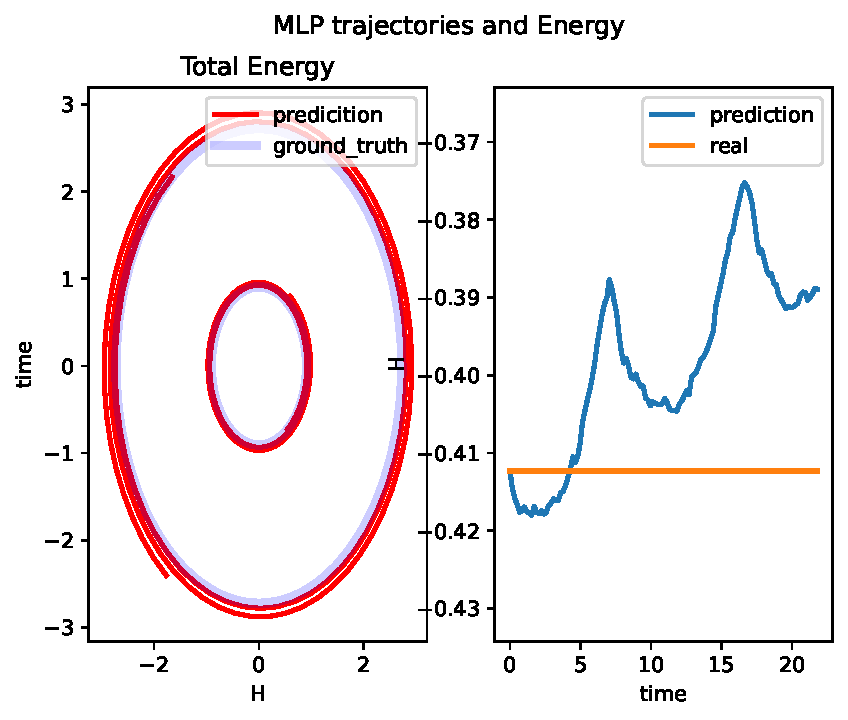
\includegraphics[width=\textwidth]{chapters/chapter5/body2_mlp_traj.pdf}
		\caption{MLP}
	\end{subfigure}
	\hfill
	\begin{subfigure}[b]{0.3\textwidth}
		\centering
		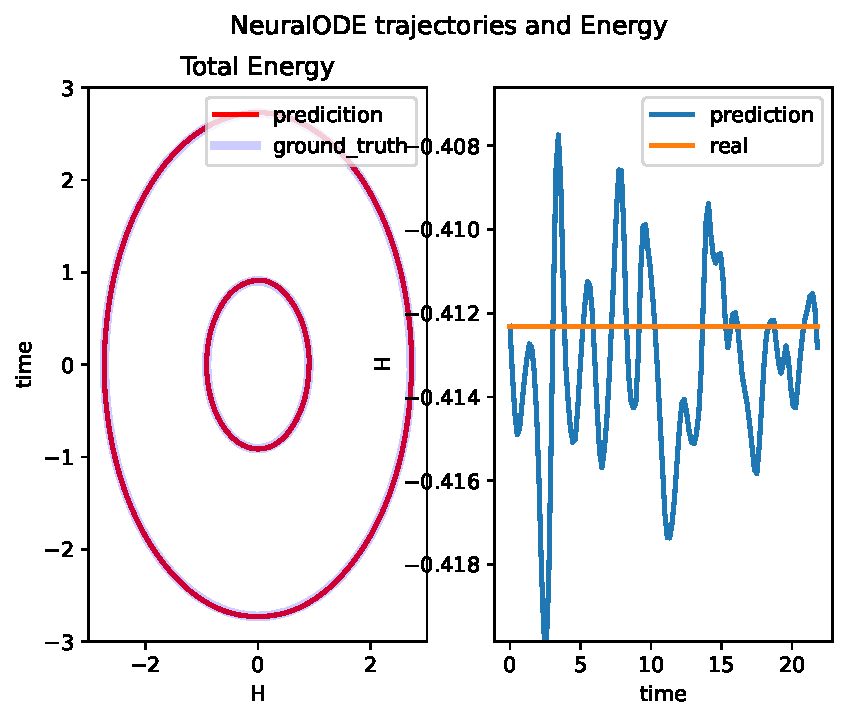
\includegraphics[width=\textwidth]{chapters/chapter5/body2_ode_traj.pdf}
		\caption{ODE}
	\end{subfigure}
	\hfill
	\begin{subfigure}[b]{0.3\textwidth}
		\centering
		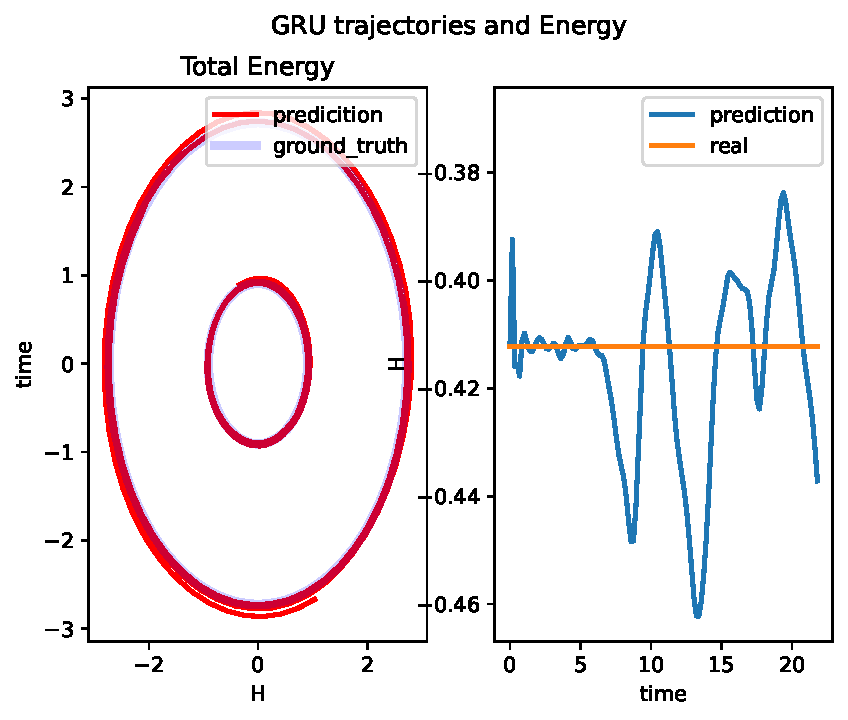
\includegraphics[width=\textwidth]{chapters/chapter5/body2_gru_traj.pdf}
		\caption{GRU}
	\end{subfigure}
	
	\vspace{0.5cm} % Adds vertical space between rows
	
	\begin{subfigure}[b]{0.3\textwidth}
		\centering
		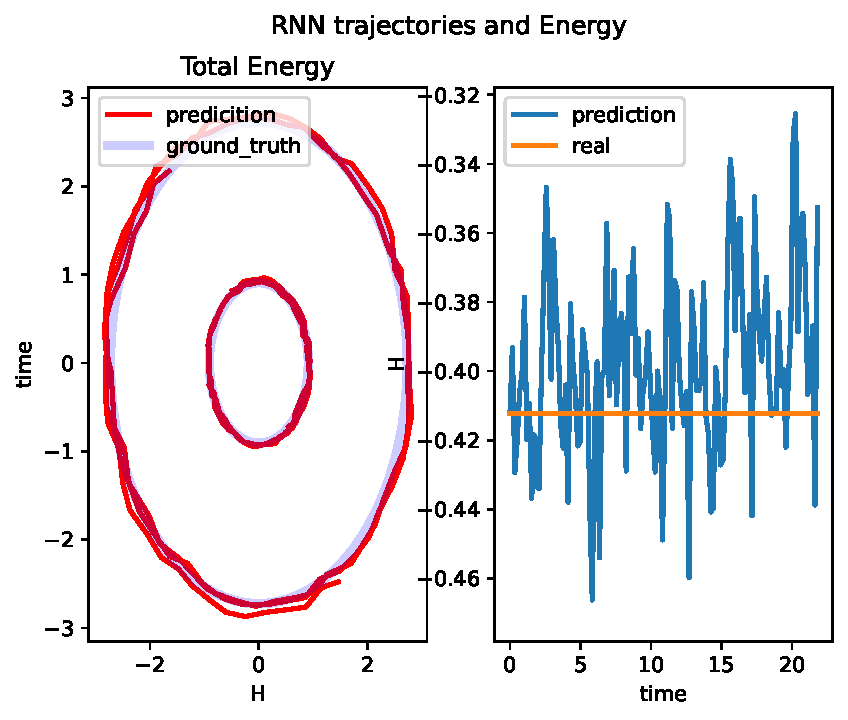
\includegraphics[width=\textwidth]{chapters/chapter5/body2_rnn_traj.pdf}
		\caption{RNN}
	\end{subfigure}
	\hfill
	\begin{subfigure}[b]{0.3\textwidth}
		\centering
		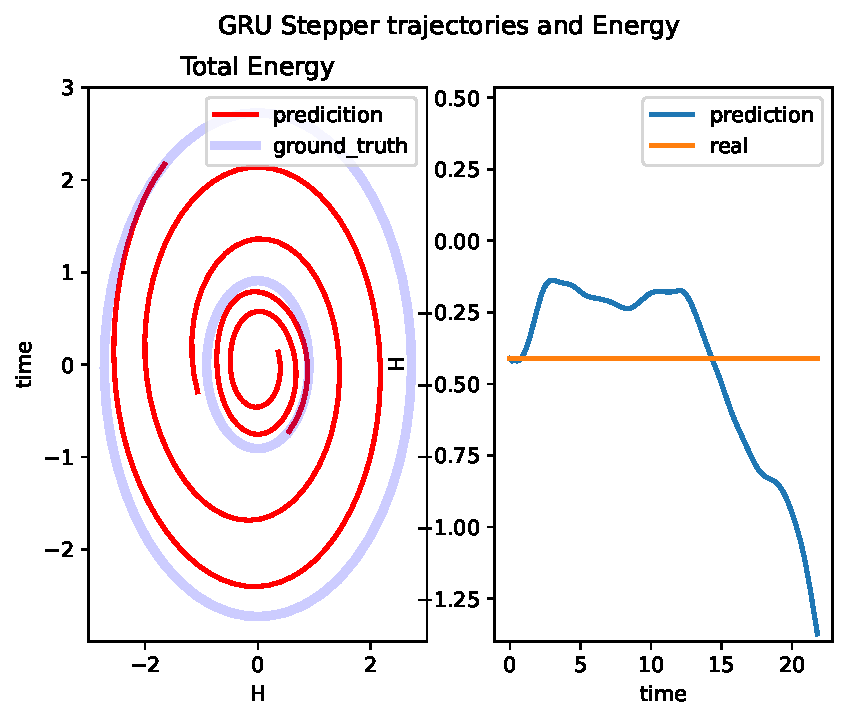
\includegraphics[width=\textwidth]{chapters/chapter5/body2_gre_traj.pdf}
		\caption{GRU Stepper}
	\end{subfigure}
	\hfill
	\begin{subfigure}[b]{0.3\textwidth}
		\centering
		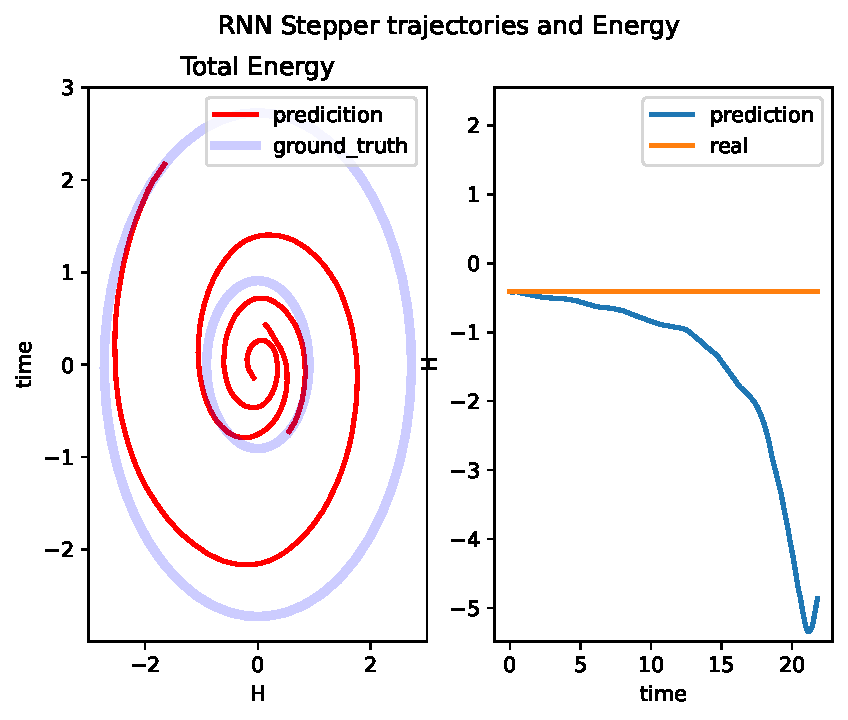
\includegraphics[width=\textwidth]{chapters/chapter5/body2_rne_traj.pdf}
		\caption{RNN stepper}
	\end{subfigure}
	
	\caption{Evaluation of the sample on the models, Trajectory and Energy(Twobody)}
	\label{body2_traj}
\end{figure}

\begin{figure}[H]
	\centering
	\begin{subfigure}[b]{0.3\textwidth}
		\centering
		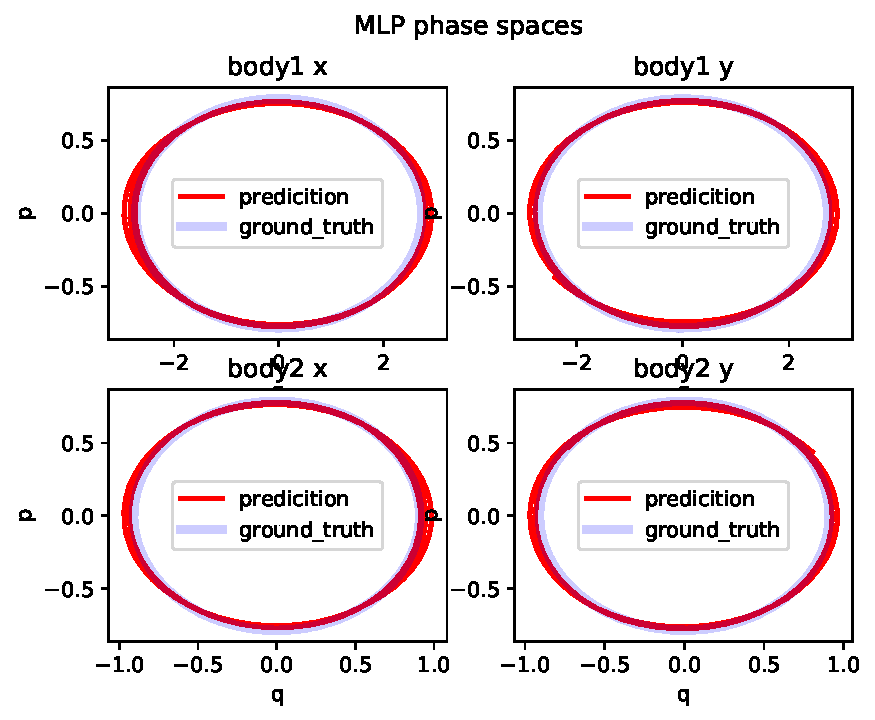
\includegraphics[width=\textwidth]{chapters/chapter5/body2_mlp_ps.pdf}
		\caption{MLP}
	\end{subfigure}
	\hfill
	\begin{subfigure}[b]{0.3\textwidth}
		\centering
		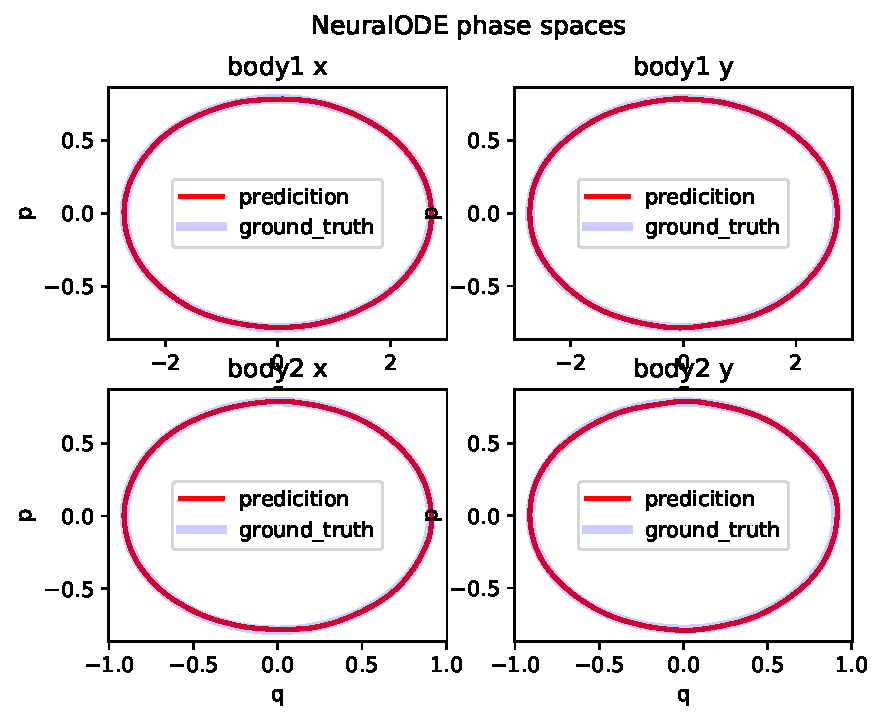
\includegraphics[width=\textwidth]{chapters/chapter5/body2_ode_ps.pdf}
		\caption{ODE}
	\end{subfigure}
	\hfill
	\begin{subfigure}[b]{0.3\textwidth}
		\centering
		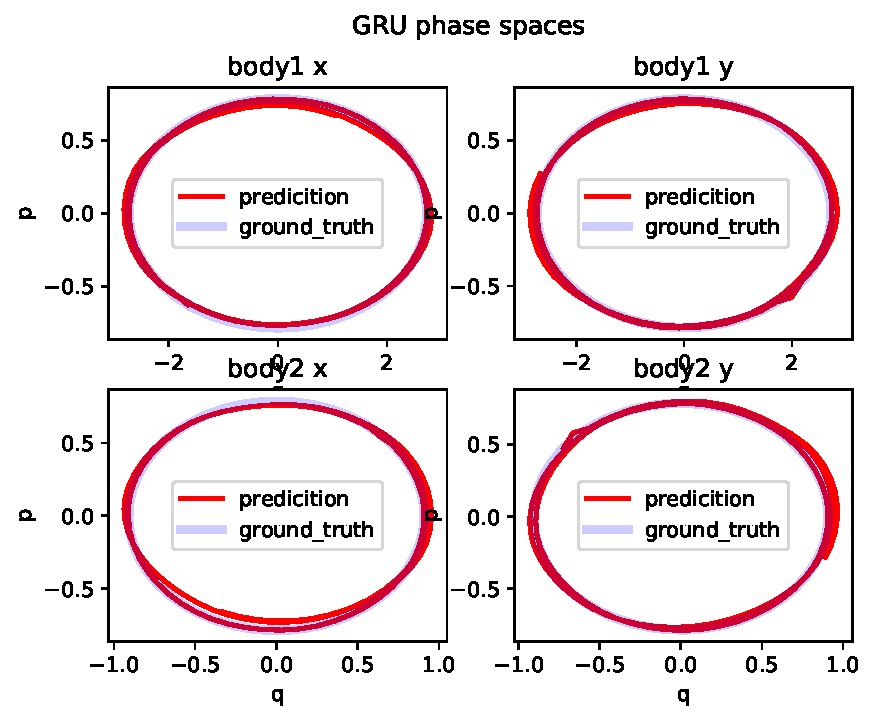
\includegraphics[width=\textwidth]{chapters/chapter5/body2_gru_ps.pdf}
		\caption{GRU}
	\end{subfigure}
	
	\vspace{0.5cm} % Adds vertical space between rows
	
	\begin{subfigure}[b]{0.3\textwidth}
		\centering
		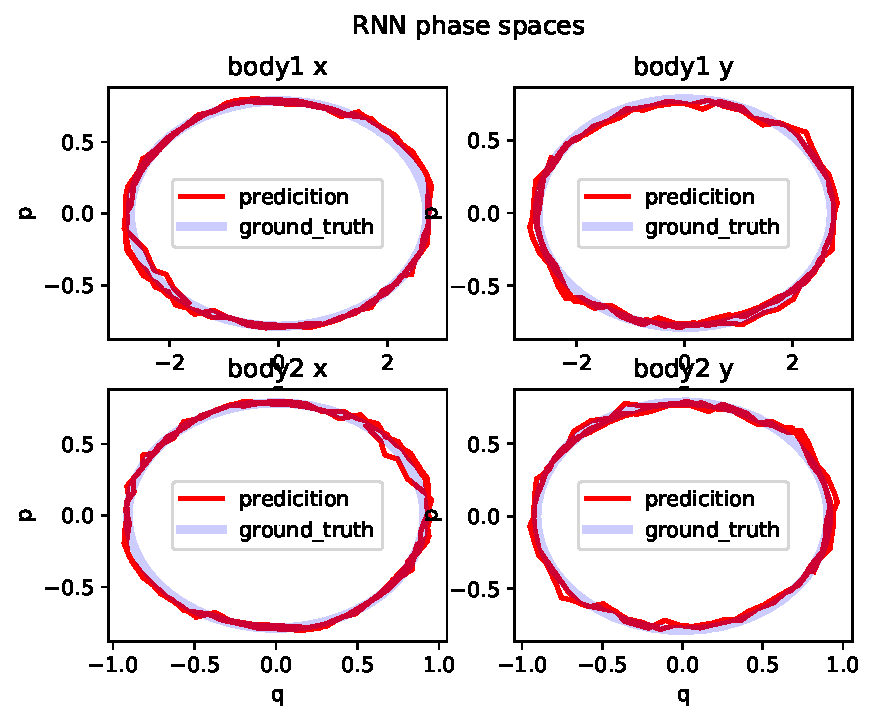
\includegraphics[width=\textwidth]{chapters/chapter5/body2_rnn_ps.pdf}
		\caption{RNN}
	\end{subfigure}
	\hfill
	\begin{subfigure}[b]{0.3\textwidth}
		\centering
		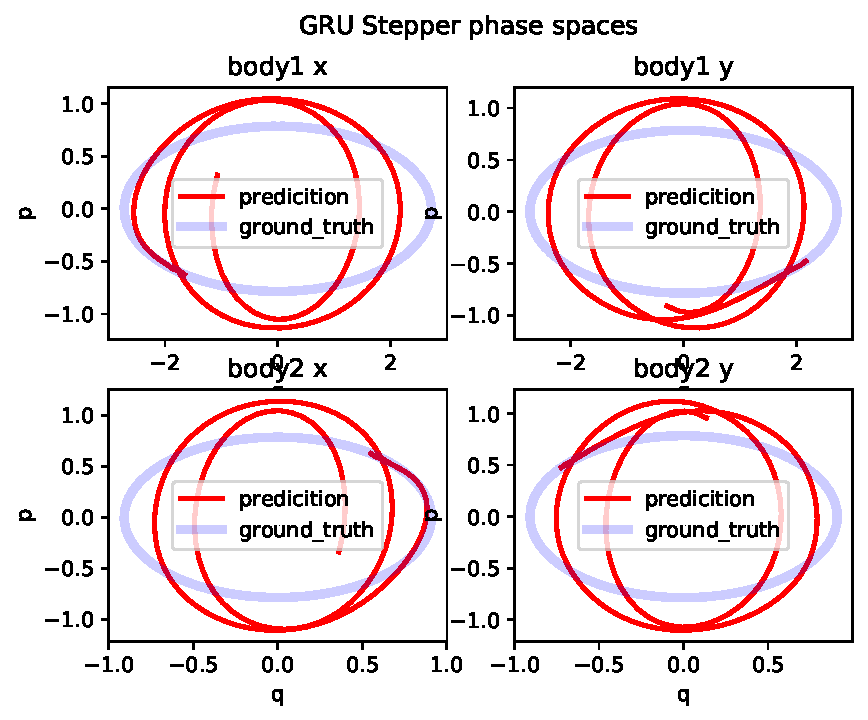
\includegraphics[width=\textwidth]{chapters/chapter5/body2_gre_ps.pdf}
		\caption{GRU Stepper}
	\end{subfigure}
	\hfill
	\begin{subfigure}[b]{0.3\textwidth}
		\centering
		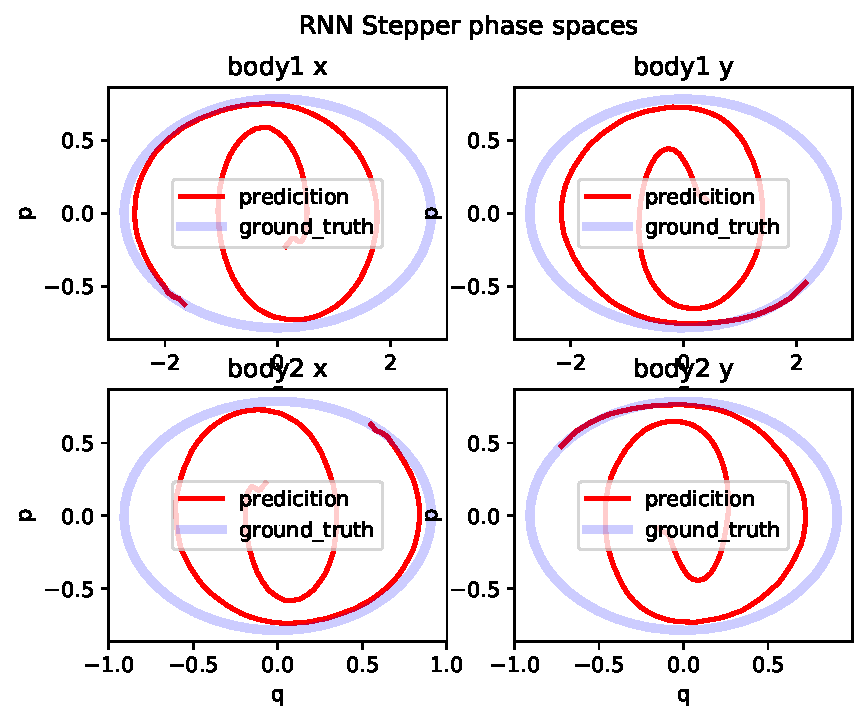
\includegraphics[width=\textwidth]{chapters/chapter5/body2_rne_ps.pdf}
		\caption{RNN stepper}
	\end{subfigure}
	
	\caption{Evaluation of the sample on the models, phase space (Twobody)}
	\label{body2_ps}
\end{figure}



\subsection{Three-body problem}
In previous chapter we discussed about creation of the Three-body Dataset.
In this Experiment we chose masses $m=\{1.0,1.0,1.0\}$ and $G=1$, we made 30 trajectories for training data and 3 trajectories for test data with 128 time points in one period.\\
The trajectories are different because we set $\alpha\in[0,1.0 \text{rad}]$ as a rotation around the origin. In this case we have same Total Energy for all trajectories\\ \begin{equation}
	\dot{\mathbf{x}} = \mathbf{A}(\mathbf{q})\mathbf{x},\text{  }\mathbf{x} = \begin{bmatrix}
		\mathbf{q}\\
		\mathbf{p}
	\end{bmatrix}
\end{equation} The matrix $\mathbf{A}$ is variational and depends strictly on position of the body in every timestep.
We used batched technique to learn the dataset and we got following results in Figures \ref{body3_loss}, \ref{body3_traj}, \ref{body3_ps}
\begin{itemize}
	\item Multilayer perceptron\\
	It trained well, Energy accuracy has gone minmal after 150 epochs of training and shows very good trajectory.

	
	\item NeuralODE\\
	Interestingly enough the trajectory on evaluation sample looks accurate but total energy doesn't look accurate. Energy accuarcy metric is after 200 epoch minimal which is good sign.´   ´

	\item GRU\\
	The model looks overtrained if we look at loss figure. Furthermore trajectory and Energy is inaccurate, but it follows the figure 8 shape. 

	\item RNN\\
	This model has failed.

	\item GRU Time Stepper\\
	It shows very good performance, similary to Neural ODE. 

	\item RNN Time Stepper\\
	It looks better then RNN but it looks like it has issues to learn for data.

\end{itemize}
From all Datasets we can conclude that RNN and RNN Stepper are bad models for the physics problems. On the other hand RNN model shows little bit of good performance but it isn't right model for this task. Through experimentations we see that NeuralODE and GRU Stepper show better performance then the baseline MLP.
\begin{figure}[H]
	\centering
	\begin{subfigure}[b]{0.3\textwidth}
		\centering
		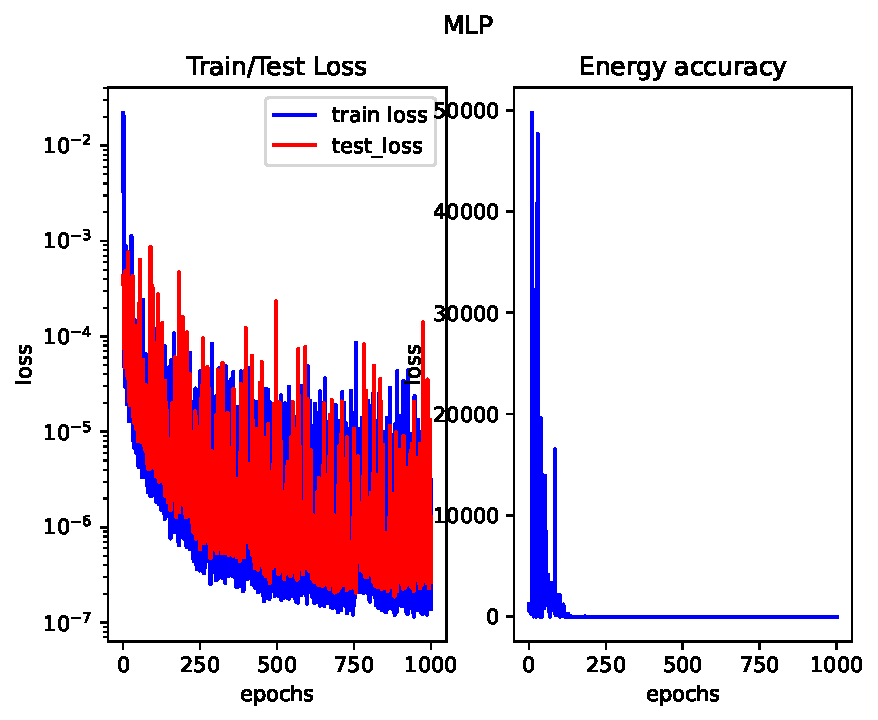
\includegraphics[width=\textwidth]{chapters/chapter5/body3_mlp_loss.pdf}
		\caption{MLP}
	\end{subfigure}
	\hfill
	\begin{subfigure}[b]{0.3\textwidth}
		\centering
		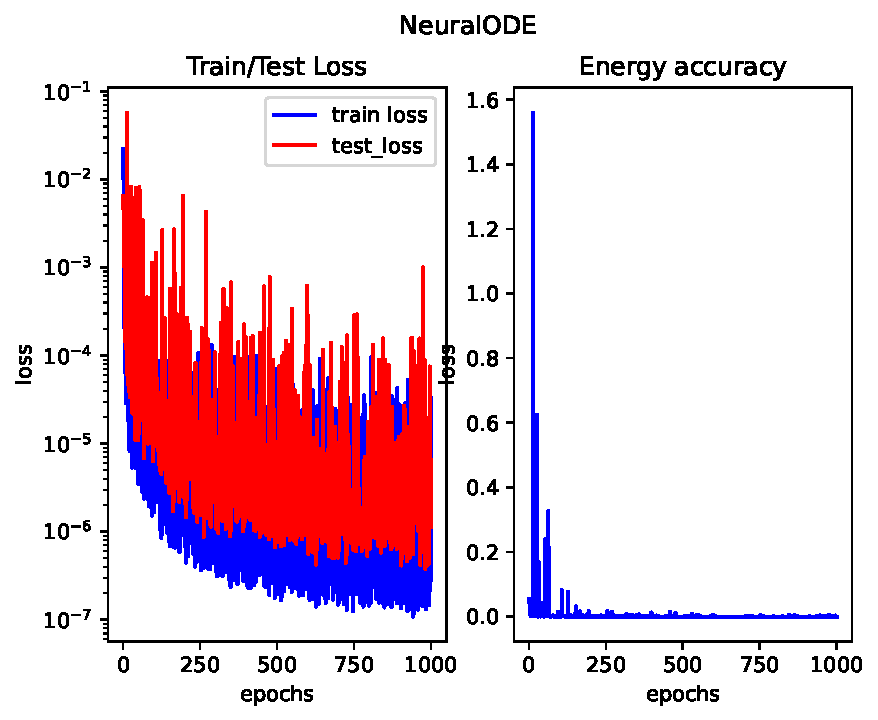
\includegraphics[width=\textwidth]{chapters/chapter5/body3_ode_loss.pdf}
		\caption{ODE}
	\end{subfigure}
	\hfill
	\begin{subfigure}[b]{0.3\textwidth}
		\centering
		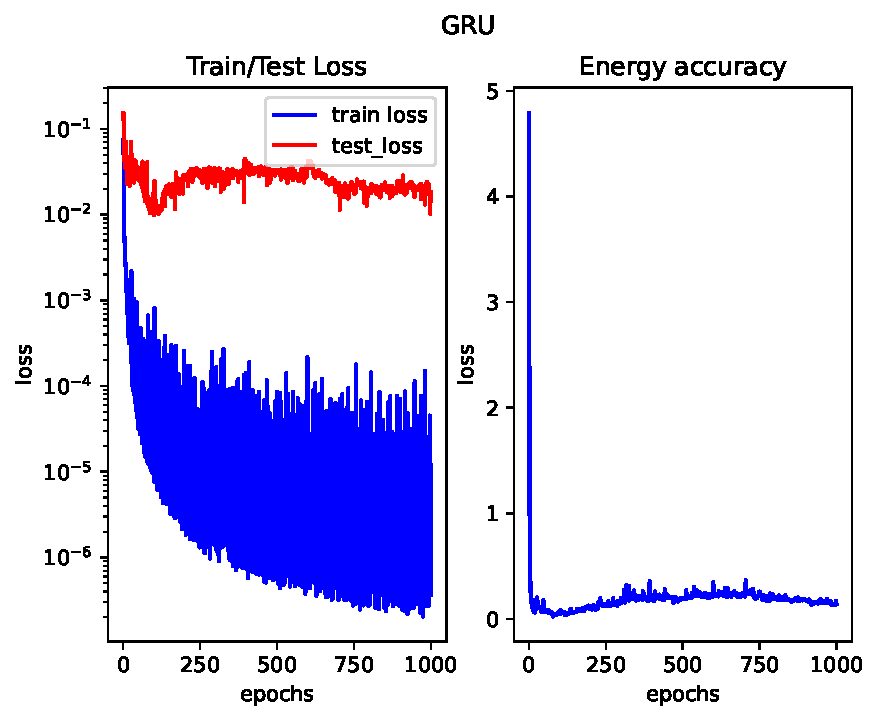
\includegraphics[width=\textwidth]{chapters/chapter5/body3_gru_loss.pdf}
		\caption{GRU}
	\end{subfigure}
	
	\vspace{0.5cm} % Adds vertical space between rows
	
	\begin{subfigure}[b]{0.3\textwidth}
		\centering
		\includegraphics[width=\textwidth]{chapters/chapter5/body3_rnn_loss.pdf}
		\caption{RNN}
	\end{subfigure}
	\hfill
	\begin{subfigure}[b]{0.3\textwidth}
		\centering
		\includegraphics[width=\textwidth]{chapters/chapter5/body3_gre_loss.pdf}
		\caption{GRU Stepper}
	\end{subfigure}
	\hfill
	\begin{subfigure}[b]{0.3\textwidth}
		\centering
		\includegraphics[width=\textwidth]{chapters/chapter5/body3_rne_loss.pdf}
		\caption{RNN stepper}
	\end{subfigure}
	
	\caption{Losses and energy accuracy on various neural models(Threebody)}
	\label{body3_loss}
\end{figure}

\begin{figure}[H]
	\centering
	\begin{subfigure}[b]{0.3\textwidth}
		\centering
		\includegraphics[width=\textwidth]{chapters/chapter5/body3_mlp_traj.pdf}
		\caption{MLP}
	\end{subfigure}
	\hfill
	\begin{subfigure}[b]{0.3\textwidth}
		\centering
		\includegraphics[width=\textwidth]{chapters/chapter5/body3_ode_traj.pdf}
		\caption{ODE}
	\end{subfigure}
	\hfill
	\begin{subfigure}[b]{0.3\textwidth}
		\centering
		\includegraphics[width=\textwidth]{chapters/chapter5/body3_gru_traj.pdf}
		\caption{GRU}
	\end{subfigure}
	
	\vspace{0.5cm} % Adds vertical space between rows
	
	\begin{subfigure}[b]{0.3\textwidth}
		\centering
		\includegraphics[width=\textwidth]{chapters/chapter5/body3_rnn_traj.pdf}
		\caption{RNN}
	\end{subfigure}
	\hfill
	\begin{subfigure}[b]{0.3\textwidth}
		\centering
		\includegraphics[width=\textwidth]{chapters/chapter5/body3_gre_traj.pdf}
		\caption{GRU Stepper}
	\end{subfigure}
	\hfill
	\begin{subfigure}[b]{0.3\textwidth}
		\centering
		\includegraphics[width=\textwidth]{chapters/chapter5/body3_rne_traj.pdf}
		\caption{RNN stepper}
	\end{subfigure}
	
	\caption{Evaluation of the sample on the models, Trajectory and Energy(Threebody)}
	\label{body3_traj}
\end{figure}

\begin{figure}[H]
	\centering
	\begin{subfigure}[b]{0.3\textwidth}
		\centering
		\includegraphics[width=\textwidth]{chapters/chapter5/body3_mlp_ps.pdf}
		\caption{MLP}
	\end{subfigure}
	\hfill
	\begin{subfigure}[b]{0.3\textwidth}
		\centering
		\includegraphics[width=\textwidth]{chapters/chapter5/body3_ode_ps.pdf}
		\caption{ODE}
	\end{subfigure}
	\hfill
	\begin{subfigure}[b]{0.3\textwidth}
		\centering
		\includegraphics[width=\textwidth]{chapters/chapter5/body3_gru_ps.pdf}
		\caption{GRU}
	\end{subfigure}
	
	\vspace{0.5cm} % Adds vertical space between rows
	
	\begin{subfigure}[b]{0.3\textwidth}
		\centering
		\includegraphics[width=\textwidth]{chapters/chapter5/body3_rnn_ps.pdf}
		\caption{RNN}
	\end{subfigure}
	\hfill
	\begin{subfigure}[b]{0.3\textwidth}
		\centering
		\includegraphics[width=\textwidth]{chapters/chapter5/body3_gre_ps.pdf}
		\caption{GRU Stepper}
	\end{subfigure}
	\hfill
	\begin{subfigure}[b]{0.3\textwidth}
		\centering
		\includegraphics[width=\textwidth]{chapters/chapter5/body3_rne_ps.pdf}
		\caption{RNN stepper}
	\end{subfigure}
	
	\caption{Evaluation of the sample on the models, phase space (Threebody)}
	\label{body3_ps}
\end{figure} 




\section{Experimentation of Physics informed datasets on three body Dataset}
After the showcase of our datasets and architectures, we will now do some training of the physics informed neural networks. We choose two datasets, one will three body problem identical to the experiment before and one dataset with mixed solutions of the body problems. We chosed carefully similar trajectories for better training performance. 
the models are:
\begin{itemize}
	\item improved Graph Hamiltonian Neural Network
	\item Hamiltonian Neural Network
	\item GRU- Graph Hamiltonian Neural Network(GAT layer)
\end{itemize}
This models are called physics informed model not only because they are made through differentiation but all of the models gives Total energy from the model directly. With this information we can make physics-informed loss. 
The physics informed-loss that we chose is
\begin{equation}
	Loss =  \omega_rMSE(\dot{\mathbf{q}},\frac{d}{dt}\hat{\mathbf{q}}) + \omega_v MSE(\dot{\mathbf{p}},\frac{d}{dt}\hat{\mathbf{p}}) +
	\omega_h MSE(H(\mathbf{q},\mathbf{p}),\hat{H}) 
\end{equation} with $[\omega_r,\omega_v,\omega_h] =1.0,1.0,0.05$.

Hyperparameters of our models:
\begin{itemize}
	\item HNN\\ 
	2 layers with tanH activation after the first layer, \\
	hidden size: 256
	\item improved GHNN\\ 
	2 GAT layers with tanH activation with dropout at attention $p=0.65$\\
	hidden size: 256\\
	output size before constructing H: 16
	\item GRUGHNN\\ 
	GRUcell + 2 GAT layers with tanH activation with dropout at attention $p=0.65$\\
	hidden size: 256\\
	output size before constructing H: 16
\end{itemize}
\subsection{Threebody dataset}
For this experiment we choosed 10 trajectories in domain $\alpha= \pi/8$. $\alpha$
is maximal angle which creates rotational region for creation of the dataset. From those 10 trajectories we made batches for training data and test data. The time sequence is 32 timepoints and 32 samples pro batch. The is $dt$=0.05.
After 100 epochs we get following results which can be observed in Figures \ref{div_traj} \ref{div_loss}.
\begin{figure}[H]
	\centering
	\begin{subfigure}[b]{0.3\textwidth}
		\centering
		\includegraphics[width=\textwidth]{chapters/chapter5/figonly_hnn_loss.pdf}
		\caption{loss at HNN}
		\label{fig:image1}
	\end{subfigure}
	\hfill
	\begin{subfigure}[b]{0.3\textwidth}
		\centering
		\includegraphics[width=\textwidth]{chapters/chapter5/figonly_ghnn_loss.pdf}
		\caption{loss at GHNN}
		\label{fig:image2}
	\end{subfigure}
	\hfill
	\begin{subfigure}[b]{0.3\textwidth}
		\centering
		\includegraphics[width=\textwidth]{chapters/chapter5/figonly_grughnn_loss.pdf}
		\caption{Loss at GRUGHNN}
		\label{fig:image3}
	\end{subfigure}
	
	\caption{Losses at various pinn models (threebody dataset)}
	\label{div_loss}
\end{figure}

% Second main plot with 3 subplots (horizontally aligned)
\begin{figure}[H]
	\centering
	\begin{subfigure}[b]{0.3\textwidth}
		\centering
		\includegraphics[width=\textwidth]{chapters/chapter5/figonly_hnn_traj.pdf}
		\caption{trajectories,phase spaces and H at HNN}
		\label{fig:image4}
	\end{subfigure}
	\hfill
	\begin{subfigure}[b]{0.3\textwidth}
		\centering
		\includegraphics[width=\textwidth]{chapters/chapter5/figonly_ghnn_traj.pdf}
		\caption{trajectories,phase spaces and H at GHNN}
		\label{fig:image5}
	\end{subfigure}
	\hfill
	\begin{subfigure}[b]{0.3\textwidth}
		\centering
		\includegraphics[width=\textwidth]{chapters/chapter5/figonly_grughnn_traj.pdf}
		\caption{trajectories,phase spaces and H at GRUGHNN}
		\label{fig:image6}
	\end{subfigure}
	
	\caption{Trajectories , phase spaces and hamiltonian at various pinn models}
	\label{div_traj}
\end{figure}

We can observe that hamiltonian is overall constant, this could be observed at HNN and improved GHNN model. Best performance shows the GRUGHNN where we have almost perfectly rollouted trajectory with almost conservative hamiltonian.

\begin{comment}

\subsection{Diverse solutions}
In this Dataset we took 5 unique diverse solutions of threebody problem. We used Figure 8\ref{diverse} as evaluation sample. First we set the time step to be $dt = 0.1$. With this information we got training and test set which is made from phase spaces on corresponding coordinates and hamiltonian value which is for every trajectory conserved. Every trajectory in the samples begins from the same coordinates under diverse moments/speeds.  

\begin{table}[H]
	\centering
	\begin{tabular}{ | c | m{5cm}| }
		\hline
		  & Specifications\\ 
		\begin{minipage}{.3\textwidth}
			\includegraphics[width=30mm, height=30mm]{chapters/chapter5/yarn}
		\end{minipage}
		&
		%\begin{minipage}[t]{5cm}
		\begin{itemize}
			\item Name : Yarn
			\item H: -1.196537
			\item T: 55.501762s
		\end{itemize}\\
		%\end{minipage}
		\hline
		  & Specifications\\ 
		\begin{minipage}{.3\textwidth}
			\includegraphics[width=30mm, height=30mm]{chapters/chapter5/fig8}
		\end{minipage}
		&
		%\begin{minipage}[t]{5cm}
		\begin{itemize}
			\item Name : Figure8
			\item H: -1.287146
			\item T: 6.324449s
		\end{itemize}\\
		%\end{minipage}
		\hline
		& Specifications\\ 
		\begin{minipage}{.3\textwidth}
			\includegraphics[width=30mm, height=30mm]{chapters/chapter5/moth}
		\end{minipage}
		&
		%\begin{minipage}[t]{5cm}
		\begin{itemize}
			\item Name : Moth
			\item H: -1.305861
			\item T: 28.670278s
		\end{itemize}\\
		%\end{minipage}
		\hline
		& Specifications\\ 
		\begin{minipage}{.3\textwidth}
			\includegraphics[width=30mm, height=30mm]{chapters/chapter5/v810}
		\end{minipage}
		&
		%\begin{minipage}[t]{5cm}
		\begin{itemize}
			\item Name : VIII 10
			\item H: -1.693544
			\item T: 48.894527s
		\end{itemize}\\
		%\end{minipage}
		\hline
		& Specifications\\ 
		\begin{minipage}{.3\textwidth}
			\includegraphics[width=30mm, height=30mm]{chapters/chapter5/googles}
		\end{minipage}
		&
		%\begin{minipage}[t]{5cm}
		\begin{itemize}
			\item Name : Googles
			\item H: -2.430116
			\item T: 10.466818s
		\end{itemize}\\
		%\end{minipage}
		\hline
	\end{tabular}
	\caption{diverse Dataset samples\cite{web}}
	\label{diverse}
\end{table}


For the models we get following plots\ref{div_loss}\ref{div_traj}
% First main plot with 3 subplots (horizontally aligned)

In those Figures we see that only GRUGHNN shows potential in training. In our evaluation trajectory plots we introduced figure 8 trajectory which wasn't in the dataset as a training sample. We know and assumpt that the trajectories won't be good or perfect. The point of this experiment was to see if those experiments are capable to make trajectories with somehow constant hamiltonian. As we see from trajectory figures our baseline achieves a constant hamiltonian value but not equal to true hamiltonian and GRUGHNN shows potential doing the same and the movement is more exaggerated but hamiliation tries to be conserved around the true value. Those models were trained for 300 epochs which equals to 1.5 days.    
\end{comment}
\subsection{Figure 8 solutions}
In this Dataset we use 4 Types of Figure 8 solutions which differs from eachother in period and energy. Those sample are in the table \ref{fig8} We use v.7.a, v.7.b, v.7.d solutions for training and testing and figure 8 for evaluation and visualization. We took 5 trajectories for every solution and it is fully supervised with loss mentioned before. Because of the size of the dataset because of different periods, we implemented stride and took every forth snapshot. The time sequences have 32 timepoints and 32 samples pro batch. \\
In figures \ref{fig_loss}, \ref{fig_traj}, we can see their loss progression, trajectories and phase spaces.

\begin{table}[H]
	\centering
	\begin{tabular}{ | c | m{5cm}| }
		\hline
		& Specifications\\ 
		\begin{minipage}{.3\textwidth}
			\includegraphics[width=30mm, height=30mm]{chapters/chapter5/v1a}
		\end{minipage}
		&
		%\begin{minipage}[t]{5cm}
		\begin{itemize}
			\item Name : v1 a/ Figure 8
			\item H: -1.287146 
			\item T: 6.324449s
		\end{itemize}\\
		%\end{minipage}
		\hline
		& Specifications\\ 
		\begin{minipage}{.3\textwidth}
			\includegraphics[width=30mm, height=30mm]{chapters/chapter5/v7a}
		\end{minipage}
		&
		%\begin{minipage}[t]{5cm}
		\begin{itemize}
			\item Name : v.7.a 
			\item H: -1.570451 
			\item T: 32.849071s
		\end{itemize}\\
		%\end{minipage}
		\hline
		& Specifications\\ 
		\begin{minipage}{.3\textwidth}
			\includegraphics[width=30mm, height=30mm]{chapters/chapter5/v7c.pdf}
		\end{minipage}
		&
		%\begin{minipage}[t]{5cm}
		\begin{itemize}
			\item Name : v.7.c
			\item H: -1.504302
			\item T: 35.043086s
		\end{itemize}\\
		%\end{minipage}
		\hline
		& Specifications\\ 
		\begin{minipage}{.3\textwidth}
			\includegraphics[width=30mm, height=30mm]{chapters/chapter5/v7d.pdf}
		\end{minipage}
		&
		%\begin{minipage}[t]{5cm}
		\begin{itemize}
			\item Name : v.7.d
			\item H: -1.080763
			\item T: 57.545253s
		\end{itemize}\\
		%\end{minipage}
		\hline
	\end{tabular}
	\caption{Figure 8 Dataset samples\cite{web}}\label{diverse}
	\label{fig8}
\end{table}

For the models we get following plots \ref{fig_loss}, \ref{fig_traj}\
% First main plot with 3 subplots (horizontally aligned)
\begin{figure}[H]
	\centering
	\begin{subfigure}[b]{0.3\textwidth}
		\centering
		\includegraphics[width=\textwidth]{chapters/chapter5/fignew_hnn_loss.pdf}
		\caption{loss at HNN}
		%\label{fig:image1}
	\end{subfigure}
	\hfill
	\begin{subfigure}[b]{0.3\textwidth}
		\centering
		\includegraphics[width=\textwidth]{chapters/chapter5/fignew_ghnn_loss.pdf}
		\caption{loss at GHNN}
	%	\label{fig:image2}
	\end{subfigure}
	\hfill
	\begin{subfigure}[b]{0.3\textwidth}
		\centering
		\includegraphics[width=\textwidth]{chapters/chapter5/fignew_grughnn_loss.pdf}
		\caption{Loss at GRUGHNN}
	%	\label{fig:image3}
	\end{subfigure}
	
	\caption{Losses at various models (figure dataset)}
	\label{fig_loss}
\end{figure}

% Second main plot with 3 subplots (horizontally aligned)
\begin{figure}[H]
	\centering
	\begin{subfigure}[b]{0.3\textwidth}
		\centering
		\includegraphics[width=\textwidth]{chapters/chapter5/fignew_hnn_traj.pdf}
		\caption{trajectories,phase spaces and H at HNN}
		%\label{fig:image4}
	\end{subfigure}
	\hfill
	\begin{subfigure}[b]{0.3\textwidth}
		\centering
		\includegraphics[width=\textwidth]{chapters/chapter5/fignew_ghnn_traj.pdf}
		\caption{trajectories,phase spaces and H at GHNN}
		%\label{fig:image5}
	\end{subfigure}
	\hfill
	\begin{subfigure}[b]{0.3\textwidth}
		\centering
		\includegraphics[width=\textwidth]{chapters/chapter5/fignew_gru_ghnn_traj.pdf}
		\caption{trajectories,phase spaces and H at GRUGHNN}
		%\label{fig:image6}
	\end{subfigure}
	
	\caption{Trajectories , phase spaces and hamiltonian at various models(figure dataset)}
	\label{fig_traj}
\end{figure}
We can clearly see that the proposed models are better then baseline HNN. They show better performance and better data fitting. Interestingly the hamiltonian on HNN and improved GHNN is almost constant and the trajectories have movement. Even though the trajectories of GRUGHNN are not accurate and hamiltonian tries to be conservative, it tries to follow the ground truthtrajectory better then other models.  



\section{Experimentation of Physics informed models on N body problem and N pendelum}
In this experiment we took only physics informed graph models. Here we have two samples of datasets for n-pendelum and n body problem. The goal of this experiment is to see if the model is capable to generalize or make correct trajectory adding or discarding one more degree of freedom. For graph neural network that shouldn't be a problem because the size of the network depends not at size of the graph but on the size of the feature space.

We will use simmilar hyperparameters for our models for both cases:
\begin{itemize}
	\item GHNN\\ 
	2 GAT layers with tanH activation with dropout at attention $p=0.65$\\
	hidden size: 128\\
	output size before constructing H: 16
	\item GRUGHNN\\ 
	GRUcell + 2 GAT layers with tanH activation with dropout at attention $p=0.65$\\
	hidden size: 128\\
	output size before constructing H: 16
\end{itemize}

\subsection{N-body pendulum}
In this case we took 20 trajectories with 128 timepoints. The dataset is created with randomised inital values: $p\_{\Theta} = 0$ and $\Theta =[-\pi,\pi]$ but we discarded those which trajectory is $|\Theta|>2\pi$. We batched training data with batch size of 32 with 32 points in trajectory, vectorfield and hamiltonian energy. We supervised within the loss
\begin{equation}
	Loss =  \omega_r(Hub({\mathbf{q}},\hat{\mathbf{q}}) + Hub({\mathbf{p}},\hat{\mathbf{p}})) +
	\omega_v(Hub(\dot{\mathbf{q}},\frac{d}{dt}\hat{\mathbf{q}}) + Hub(\dot{\mathbf{p}},\frac{d}{dt}\hat{\mathbf{p}})) +
	\omega_h Hub(H(\mathbf{q},\mathbf{p}),\hat{H}) 
\end{equation} with $\omega ={1.00,0.5,0.1}$.
\begin{table}[h!]
	\centering
	\caption{Evaluation of 3dof sample on various models and training procedures} % Add your caption here
	\label{tab:my_label}               % Add your label here
	\begin{tabular}{|l|l|l|l|}
		\hline
		dof3 & roll & vec & h\\ 
		\hline
		HGNN 3dof & 8.58 & 22.91 & 0.57 \\  
		\hline
		HGNN 4dof & 150.74 & 501.93 & 10.93 \\  
		\hline
		GRUHGNN 3dof & 2.57 & 21,7211 & 6,7363 \\  
		\hline
		GRUHGNN 4dof & 5.6 & 29.85 & 5.96 \\  
		\hline
	\end{tabular}
\end{table}
\begin{table}[h!]
	\centering
	\caption{Evaluation of 4dof sample on various models and training procedures} % Add your caption here
	\label{tab:my_label}               % Add your label here
	\begin{tabular}{|l|l|l|l|}
		\hline
		dof4 & roll & vec & h\\ 
		\hline
		HGNN 3dof & 12.35 & 31.85 & 2.12 \\  
		\hline
		HGNN 4dof & 10.45 & 32.28 & 22.9 \\  
		\hline
		GRUHGNN 3dof & 5.61 & 24.72 & 10.71 \\  
		\hline
		GRUHGNN 4dof & 7.00 & 33.1747 & 12.5609 \\  
		\hline
	\end{tabular}
\end{table}






\begin{figure}[H]
	\centering
	\begin{subfigure}[b]{0.4\textwidth}
		\centering
		\includegraphics[width=\textwidth]{chapters/chapter5/loss_3dof.pdf}
		\caption{Losses at 3dof training}
		%\label{fig:image4}
	\end{subfigure}
	\hfill
	\begin{subfigure}[b]{0.4\textwidth}
		\centering
		\includegraphics[width=\textwidth]{chapters/chapter5/loss_4dof.pdf}
		\caption{Losses at 4dof training}
		%\label{fig:image5}
	\end{subfigure}
	
	
	\caption{Losses till 500 epochs(Pendulum)}
	\label{fig_traj}
\end{figure}
\begin{table}[h!]
\centering
\caption{Evaluation of 3dof sample on GRUGNN and training procedures} % Add your caption here
\label{tab:pend500}               % Add your label here
\begin{tabular}{|l|l|l|l|l|}
	\hline
	dof3 & roll & vec & h\\ 
	\hline
	GRUHGNN 3dof & 3.49 & 23,17 & 7.7 \\  
	\hline
	GRUHGNN 4dof & 6.71 & 26.6007 & 45.09 \\  
	\hline
\end{tabular}
\end{table}



\begin{table}[h!]
\centering
\caption{Evaluation of 4dof sample on GRUGNN models and training procedures, } % Add your caption here
\label{tab:pend1000}               % Add your label here
\begin{tabular}{|l|l|l|l|l|}
	\hline
	dof4 & roll & vec & h\\  
	\hline
	GRUHGNN 3dof & 59.33 & 24.95 & 20.82 \\  
	\hline
	GRUHGNN 4dof & 8.47 & 26.8 & 50.2 \\  
	\hline
\end{tabular}
\end{table}

\begin{figure}[H]
	\centering
	\begin{subfigure}[b]{0.4\textwidth}
		\centering
		\includegraphics[width=\textwidth]{chapters/chapter5/loss_3dof1000.pdf}
		\caption{Losses at 3dof training}
		%\label{fig:image4}
	\end{subfigure}
	\hfill
	\begin{subfigure}[b]{0.4\textwidth}
		\centering
		\includegraphics[width=\textwidth]{chapters/chapter5/loss_4dof1000.pdf}
		\caption{Losses at 4dof training}
		%\label{fig:image5}
	\end{subfigure}
	
	
	\caption{Losses till 1000 epochs on GRUGHNN(Pendelum)}
	\label{fig_traj}
\end{figure}

\begin{figure}[htbp]
	\centering
	% First row of subplots
	\begin{subfigure}[b]{0.45\textwidth}
		\centering
		\includegraphics[width=\textwidth]{chapters/chapter5/traj_3dof3_pend.pdf} % Replace with your image file
		\caption{GRUGHNN trained on 3dof sample and made 3dof trajectory}
		\label{fig:sub1}
	\end{subfigure}
	\hfill
	\begin{subfigure}[b]{0.45\textwidth}
		\centering
		\includegraphics[width=\textwidth]{chapters/chapter5/traj_4dof3_pend.pdf} % Replace with your image file
		\caption{GRUGHNN trained on 4dof sample and made 3dof trajectory}
		\label{fig:sub2}
	\end{subfigure}
	
	% Second row of subplots
	\vspace{0.5cm}
	\begin{subfigure}[b]{0.45\textwidth}
		\centering
		\includegraphics[width=\textwidth]{chapters/chapter5/traj_3dof4_pend.pdf} % Replace with your image file
		\caption{GRUGHNN trained on 3dof sample and made 4dof trajectory}
		\label{fig:sub3}
	\end{subfigure}
	\hfill
	\begin{subfigure}[b]{0.45\textwidth}
		\centering
		\includegraphics[width=\textwidth]{chapters/chapter5/traj_4dof4_pend.pdf} % Replace with your image file
		\caption{GRUGHNN trained on 4dof sample and made 4dof trajectory}
		\label{fig:sub4}
	\end{subfigure}
	
	\caption{trajectories of pendelums after 1000 epochs}
	\label{pend_traj}
\end{figure}

In the tables \ref{tab:pend500} and  \ref{tab:pend1000} we compared the HuberLoss values of evaluation trajectoriy of 3dof pendulum and 4dof pendelum on the models PINN under 500 epochs  and 1000 epochs only on GRUGHNN. Chosed trajectory is fully unknown to the models.\\ 
eFrom the values we can read that GHNN dosen't like losing degree of freedom. We see very big difference in those values. In other cases there is difference but not exaggerated.\\
The trajectories are observable in figure \ref{pend_traj}

\subsection{N-body problem}
In the similar manner as N-pendelum we made N-body Problem.
First we needed to set up domain of movement and we chosed 20 samples of trajectories of 128 timesteps with $dt =0.01$. In the dataset we have position velocity and energy and it is suprivised same as N-pendelum case and we reused only GRUGHNN model because it showed greatest performance in last experiments. This is just proof of concept that adding and discarding the graph nodes is possible.
\begin{table}[h!]
	\centering
	\caption{Evaluation of 3dof sample on GRUGNN and training procedures, (Nbody)} % Add your caption here
	\label{tab:my_label}  
\begin{tabular}{|l|l|l|l|l|}
	\hline
	dof3 & roll & vec & h\\  
	\hline
	GRUHGNN 3dof & 0.88 & 9.19 & 6.03 \\  
	\hline
	GRUHGNN 4dof & 0.87 & 6.97 & 5.81 \\  
	\hline
\end{tabular}
\end{table}

\begin{table}[h!]
	\centering
	\caption{Evaluation of 4dof sample on GRUGNN and training procedures (Nbody)} % Add your caption here
	\label{tab:my_label}  
\begin{tabular}{|l|l|l|l|l|}
	\hline
	dof4 & roll & vec & h\\  
	\hline
	GRUHGNN 3dof & 1.25 & 7.39 & 9.37 \\  
	\hline
	GRUHGNN 4dof & 1.08 & 10.11 & 9.37 \\  
	\hline
\end{tabular}
\end{table}



\begin{figure}[H]
	\centering
	\begin{subfigure}[b]{0.4\textwidth}
		\centering
		\includegraphics[width=\textwidth]{chapters/chapter5/loss_9.pdf}
		\caption{Losses at 9 bodies training}
		%\label{fig:image4}
	\end{subfigure}
	\hfill
	\begin{subfigure}[b]{0.4\textwidth}
		\centering
		\includegraphics[width=\textwidth]{chapters/chapter5/loss_10.pdf}
		\caption{Losses at 10 bodies training}
		%\label{fig:image5}
	\end{subfigure}
	
	
	\caption{Losses till 1000 epochs on GRUGHNN (Nbody)}
	\label{fig_traj}
\end{figure}

\begin{figure}[htbp]
	\centering
	% First row of subplots
	\begin{subfigure}[b]{0.45\textwidth}
		\centering
		\includegraphics[width=\textwidth]{chapters/chapter5/traj_9dof_9.pdf} % Replace with your image file
		\caption{GRUGHNN trained on 9dof sample and made 9dof trajectory}
		\label{fig:sub1}
	\end{subfigure}
	\hfill
	\begin{subfigure}[b]{0.45\textwidth}
		\centering
		\includegraphics[width=\textwidth]{chapters/chapter5/traj_10dof_9.pdf} % Replace with your image file
		\caption{GRUGHNN trained on 10dof sample and made 9dof trajectory}
		\label{fig:sub2}
	\end{subfigure}
	
	% Second row of subplots
	\vspace{0.5cm}
	\begin{subfigure}[b]{0.45\textwidth}
		\centering
		\includegraphics[width=\textwidth]{chapters/chapter5/traj_9dof_10.pdf} % Replace with your image file
		\caption{GRUGHNN trained on 9dof sample and made 10dof trajectory}
		\label{fig:sub3}
	\end{subfigure}
	\hfill
	\begin{subfigure}[b]{0.45\textwidth}
		\centering
		\includegraphics[width=\textwidth]{chapters/chapter5/traj_10dof_10.pdf} % Replace with your image file
		\caption{GRUGHNN trained on 10dof sample and made 10dof trajectory}
		\label{fig:sub4}
	\end{subfigure}
	\caption{Trajectories of nbody after 1000 epochs}
	\label{fig:body_Traj}
\end{figure}

\begin{figure}[htbp]
	\centering
	\includegraphics[width=0.8\textwidth]{chapters/chapter5/nbody_hamiltonian.pdf} % Replace with the path to your image file
	\caption{Hamiltonian of nbody cases}
	\label{nbody_ham}
\end{figure}

The results of the adding and discarding a body are really suprising good enough. Still the model tolerates more losing the body then gain it. This can be observed in \ref{body_traj} It is fully understandable looking at Nbody problem. Adding a body we could heavy disrupt the system.
Mostly interesting result is hamiltonian figure \ref{nbody_ham}
With those experiments we got an good insight in those PINN models.
\chapter{Conclusions}
Physics-informed neural networks showed great capability in learning hamiltonian systems directly from data, though the graph structure of GNNs presented a really interesting alternative to classic multilayer perceptrons. The main challenges for those models remain being computationally demanding and requiring huge, high-quality datasets. Most of the experiments we showed in this thesis would never have been possible with a normal-end PC, hence underlining how access to high-performance computing resources played a an important role, for instance, using the Lichtenberg Cluster and high-end Laptop.\\
In this study, we successfully generated datasets from the hamiltonian equations and subsequently demonstrated that most of state of the art models  can learn from the time-series data. This provides further evidence of the  data-driven models can encapsulate complicated physical systems.\\
Through the experiments we demonstrated the performance of physics-informed models and  tested our own models on our datasets. Although the results weren't 100 \% accurate enough due to hardware issues we managed to obtain promising outcomes.  

In addition, we envision future studies on the Kolmogorov-Arnold Networks, since this is a newly proposed architecture that blends graph structures with spline functions that have a learned shape as a parameter to model natural data. Preliminary studies suggest KAN can learn physics-based systems and partial differential equations, which would represent a potentially strong alternative to traditional MLPs and GNNs\cite{kan}. In essence, KAN may prove to be that key leap forward that the domain of physical machine learning is pushing for.
   
%\chapter{Appendix}
\begin{appendices}
	
	% Start appendix sections using \section
	\renewcommand{\thesection}{A\arabic{section}}  % This will format sections as A1, A2, A3, ...
	
	\section{Oscilator code}
\begin{lstlisting}[language=Python, caption={ocilator.py}]
	"""
	class which creates matrix vector multiplication for trajectory rollout
	k: stiffness coeficient
	m: mass
	"""
	class oscigradH(nn.Module):
	def __init__(self,k,m):
	super(oscigradH,self).__init__()
	self.A=torch.zeros(2,2).to(device_util.DEVICE)
	self.A[0,1]=1/m
	self.A[1,0]=-k
	
	def forward(self,t,y):
	return torch.matmul(y,self.A.T)
	"""
	class to create an oscilator data
	k: stiffness coeficient
	m: mass
	
	"""    
	class oscilator:
	def __init__(self,m,k):
	self.k = k
	self.m = m
	self.F = oscigradH(k,m).to(device_util.DEVICE)
	"""
	method for period T
	"""
	def getT(self):
	return 2*math.pi/math.sqrt(self.k/self.m)
	
	
	"""
	method for creating randomly initial values for the oscilator
	samples : number of initial values
	H_span : region for the energy
	"""	
	def make_inits(self,samples,H_span=[1,5]):
	Hs = H_span[0]*torch.rand(samples,)*(H_span[1]-H_span[0])
	a = torch.sqrt(2*self.m*Hs)
	b = torch.sqrt(2*Hs/self.k)
	phis = torch.rand(samples,)*2*torch.pi
	
	p = a * torch.cos(phis)
	p = torch.unsqueeze(p,dim=-1)
	
	x = b * torch.sin(phis)
	x = torch.unsqueeze(x,dim=-1)
	
	return torch.cat((x,p),dim=-1)
	"""
	method for calculating hamitlonian
	
	returns: hamiltonian
	"""
	def hamiltonian(self,dataset):
	# dataset type [len(t),batches,1,2], [len(t),1,2], [batches,1,2]
	if dataset.dim() > 3:
	dataset = dataset.squeeze()
	if dataset.dim() < 3:
	dataset = torch.unsqueeze(dataset,dim=1)
	x = dataset[:,:,0]
	p = dataset[:,:,1]
	
	T = p.square()/(2*self.m)
	U = self.k*x.square()/2
	
	H = T+U
	return H
	
	"""
	method for creating only one trajectory
	points: number of time points, sequence length
	H_span: region for the energy
	
	returns: trajectory and time
	"""
	def make_one(self,points, H_span=[1,5]):
	omega = math.sqrt(self.k/self.m)
	T = 2*math.pi/omega
	
	t = torch.linspace(0,T,points).to(device_util.DEVICE)
	y=self.make_inits(1,H_span=H_span).to(device_util.DEVICE)
	data = odeint(self.F,y[0,:],t,method="rk4")
	
	return data.unsqueeze(dim=1), t
	"""
	method for creating the dataset 
	points: number of time points,sequence length
	samples : number of initial values
	T: period if 0, else end time
	H_span: region for the energy
	
	returns: trajectory and time
	"""
	def make_dataset(self,points,samples,T = 0,H_span=[1,5]):
	if T == 0:
	omega = math.sqrt(self.k/self.m)
	T = 2*math.pi/omega
	t = torch.linspace(0,T,points).to(device_util.DEVICE)
	y=self.make_inits(samples,H_span=H_span).to(device_util.DEVICE)
	y=torch.unsqueeze(y,dim=1)
	print(y.shape)
	data = odeint(self.F,y,t,method="rk4")
	
	return data, t
\end{lstlisting}
	
	\section{Twobody code}
	\begin{lstlisting}[language=Python, caption={ocilator.py}]
		"""
		class which creates matrix vector multiplication for trajectory rollout
		k: stiffness coeficient
		m: mass
		"""
		class oscigradH(nn.Module):
		def __init__(self,k,m):
		super(oscigradH,self).__init__()
		self.A=torch.zeros(2,2).to(device_util.DEVICE)
		self.A[0,1]=1/m
		self.A[1,0]=-k
		
		def forward(self,t,y):
		return torch.matmul(y,self.A.T)
		"""
		class to create an oscilator data
		k: stiffness coeficient
		m: mass
		
		"""    
		class oscilator:
		def __init__(self,m,k):
		self.k = k
		self.m = m
		self.F = oscigradH(k,m).to(device_util.DEVICE)
		"""
		method for period T
		"""
		def getT(self):
		return 2*math.pi/math.sqrt(self.k/self.m)
		
		
		"""
		method for creating randomly initial values for the oscilator
		samples : number of initial values
		H_span : region for the energy
		"""	
		def make_inits(self,samples,H_span=[1,5]):
		Hs = H_span[0]*torch.rand(samples,)*(H_span[1]-H_span[0])
		a = torch.sqrt(2*self.m*Hs)
		b = torch.sqrt(2*Hs/self.k)
		phis = torch.rand(samples,)*2*torch.pi
		
		p = a * torch.cos(phis)
		p = torch.unsqueeze(p,dim=-1)
		
		x = b * torch.sin(phis)
		x = torch.unsqueeze(x,dim=-1)
		
		return torch.cat((x,p),dim=-1)
		"""
		method for calculating hamitlonian
		
		returns: hamiltonian
		"""
		def hamiltonian(self,dataset):
		# dataset type [len(t),batches,1,2], [len(t),1,2], [batches,1,2]
		if dataset.dim() > 3:
		dataset = dataset.squeeze()
		if dataset.dim() < 3:
		dataset = torch.unsqueeze(dataset,dim=1)
		x = dataset[:,:,0]
		p = dataset[:,:,1]
		
		T = p.square()/(2*self.m)
		U = self.k*x.square()/2
		
		H = T+U
		return H
		
		"""
		method for creating only one trajectory
		points: number of time points, sequence length
		H_span: region for the energy
		
		returns: trajectory and time
		"""
		def make_one(self,points, H_span=[1,5]):
		omega = math.sqrt(self.k/self.m)
		T = 2*math.pi/omega
		
		t = torch.linspace(0,T,points).to(device_util.DEVICE)
		y=self.make_inits(1,H_span=H_span).to(device_util.DEVICE)
		data = odeint(self.F,y[0,:],t,method="rk4")
		
		return data.unsqueeze(dim=1), t
		"""
		method for creating the dataset 
		points: number of time points,sequence length
		samples : number of initial values
		T: period if 0, else end time
		H_span: region for the energy
		
		returns: trajectory and time
		"""
		def make_dataset(self,points,samples,T = 0,H_span=[1,5]):
		if T == 0:
		omega = math.sqrt(self.k/self.m)
		T = 2*math.pi/omega
		t = torch.linspace(0,T,points).to(device_util.DEVICE)
		y=self.make_inits(samples,H_span=H_span).to(device_util.DEVICE)
		y=torch.unsqueeze(y,dim=1)
		print(y.shape)
		data = odeint(self.F,y,t,method="rk4")
		
		return data, t
	\end{lstlisting}
	
	
	\section{threebody code}

	
\end{appendices}






\printbibliography

\end{document}
